\documentclass[a4paper,12pt]{report}

\newcommand{\nameInitial}{
    \textcolor{black}{W. Viljoen}  %change colour to black and enter your initial and surname
}
\newcommand{\nameFull}{
    \textcolor{black}{Willem Viljoen} %change colour to black and enter your firstname and surname
}
\newcommand{\stNumber}{
    \textcolor{black}{22877169} %change to black and enter your student number 
}
\newcommand{\myDate}{\textcolor{black}{November 1, 2023} %change colour and if you want to date.
}
\newcommand{\signature}{frontmatter/fig/Signature}   %Upload your signature as "frontmatter/fig/Signature.png"


%%%%%%%%%%%%%%%%%%%%%%%%%%%%%%%%%%%%%%%%%%%%%%%%%%%%%%%%%%%%%%%%%
%From here you can ignore up to \begin{document} (line 107)
%%%%%%%%%%%%%%%%%%%%%%%%%%%%%%%%%%%%%%%%%%%%%%%%%%%%%%%%%%%%%%%%%
% Page layout
\usepackage[left=2.5cm,right=2.5cm,top=2.5cm,bottom=2.5cm]{geometry}
% Figures
\usepackage[margin=\the\parindent,small,bf,sf]{caption}
\usepackage{graphicx}
\usepackage{pdfpages}
\setlength{\abovecaptionskip}{7.5pt}  % spacing above and below captions
\newcommand*{\WaterMark}[2][0.2\paperwidth]{\AddToShipoutPicture*{\AtTextCenter{\parbox[c]{0pt}{\makebox[0pt][c]{\includegraphics[width=#1]{#2}}}}}}
\usepackage{subcaption}
% Font and text
\usepackage[afrikaans,english]{babel}
\usepackage{microtype}
\usepackage{setspace}
\usepackage{lmodern}
\newcommand{\myemph}[1]{{\sffamily\bfseries#1}}
\sloppy
\onehalfspacing
\usepackage{siunitx}
\usepackage{lipsum}
% Headings
\usepackage[raggedright,sf,bf]{titlesec}
\usepackage{titlesec}
\usepackage{titletoc}
\titlelabel{\thetitle.\ }
% Modify chapter formatting
\titleformat{\chapter}[display]
{\normalfont\huge\bfseries}{}{0pt}{\vspace{-40pt}\Huge}
\titlespacing*{\chapter}{0pt}{-30pt}{20pt}
% Table of contents
\makeatletter
\let\originall@chapter\l@chapter
\def\l@chapter#1#2{\originall@chapter{{\sffamily #1}}{#2}}
\makeatother
\let \savenumberline \numberline
\def \numberline#1{\savenumberline{#1.}}
% Mathematics
\usepackage[cmex10]{amsmath}
\usepackage{amssymb}
\usepackage{cancel}
\DeclareMathOperator*{\argmax}{arg\,max}
\newcommand{\T}{^\textrm{T}}
\newcommand{\tr}{\textrm{tr}}
\renewcommand{\vec}[1]{\boldsymbol{\mathbf{#1}}}
\newcommand{\defeq}{\triangleq}
% Tables
\usepackage{booktabs}
\usepackage{tabularx}
\usepackage{multirow}
\newcommand{\mytable}{
    \centering
    \small
    \renewcommand{\arraystretch}{1.2}
    }
\renewcommand{\tabularxcolumn}[1]{m{#1}}
\newcolumntype{C}{>{\centering\arraybackslash}X}
\newcolumntype{L}{>{\raggedright\arraybackslash}X}
% Header and footer
\usepackage{fancyhdr}
\pagestyle{fancy}
\fancyhf{}
\renewcommand{\sectionmark}[1]{\markright{\normalsize \thesection.\ #1}}
\fancyhead[C]{\nouppercase{\textit{\rightmark}}}
\fancyhead[RO]{\thepage}
% \fancyhead[LE]{\thepage}  % double-sided printing
\fancyfoot{}
\setlength\headheight{14.5pt}
\renewcommand{\headrulewidth}{0pt}
\fancypagestyle{plain}{\fancyhead{}
                       \renewcommand{\headrulewidth}{0pt}
                       \fancyfoot[C]{\thepage}}
% Pseudo-code
\usepackage{algorithm}  % should go before \usepackage{hyperref}
% Table of contents and hyperlinks
\usepackage{hyperref}
\hypersetup{colorlinks=true,linktoc=all,citecolor=black,linkcolor=black}
\usepackage[nottoc]{tocbibind}
% Pseudo-code
\usepackage{algpseudocode}  % should go after \usepackage{hyperref}
\renewcommand{\thealgorithm}{\arabic{chapter}.\arabic{algorithm}} 
% Bibliography
\usepackage{cite}  % automatically reorder inline citations
\bibliographystyle{IEEEtran}
% Fix titlesec issue
\usepackage{etoolbox}
\makeatletter
\patchcmd{\ttlh@hang}{\parindent\z@}{\parindent\z@\leavevmode}{}{}
\patchcmd{\ttlh@hang}{\noindent}{}{}{}
\makeatother
 \usepackage[normalem]{ulem}
%%%%%%%%%%%%%%%%%%%%%%%%%%%%%%%%%%%%%%%%%%%%%%%%%%%%%%%%%%%%%%%%%
% Ignore up to here. 
%%%%%%%%%%%%%%%%%%%%%%%%%%%%%%%%%%%%%%%%%%%%%%%%%%%%%%%%%%%%%%%%%

\begin{document}

% Front matter
\graphicspath{{frontmatter/fig/}}
\pagenumbering{Alph}

\begin{titlepage}
\begin{center}


\includegraphics[width=8cm]{frontmatter/fig/SU_logo_RGB_without_slogan.pdf}

\vfill

		{\sffamily \bfseries \huge a Modular Battery Management System for LFP Batteries \par}
		
		\vspace{7em}
		
		{\large {\Large  Willem Viljoen} \\ 22877169 \par}

		
		\vspace{8em}
		
		{Report presented in partial fulfilment of the requirements for the degree of Electrical Engineering in the Faculty of Engineering at Stellenbosch University. \par}
		
		\vfill
  
        {\large {Supervisor}: Dr JM\ Strauss \par}		
		{Department of Electrical and Electronic Engineering \par}

\vfill


%{\large {Supervisor}: Dr L. Skywalker} %\\
% Department of Electrical and Electronic Engineering \par}

\vfill

{\Large \myDate}
\end{center}
\end{titlepage}

\pagenumbering{roman}
%\chapter*{Declaration}
\newpage
\pagestyle{plain}
\addcontentsline{toc}{chapter}{Declaration}
\makeatletter\@mkboth{}{Declaration}\makeatother

\centerline{
\includegraphics[width=8cm]{frontmatter/fig/SU_horizontal_RGB.pdf}}
\vspace*{-10pt}

\section*{\centering Plagiaatverklaring / \textit{Plagiarism Declaration}}

\vspace*{5pt}

\begin{enumerate}
    \item Plagiaat is die oorneem en gebruik van die idees, materiaal en ander intellektuele eiendom van ander persone asof dit jou eie werk is.\\
    \textit{Plagiarism is the use of ideas, material and other intellectual property of another's work
        and to present is as my own.}
    
    \item Ek erken dat die pleeg van plagiaat 'n strafbare oortreding is aangesien dit 'n vorm van diefstal is.\\
    \textit{I agree that plagiarism is a punishable offence because it constitutes theft.}
    
    \item Ek verstaan ook dat direkte vertalings plagiaat is. \\
    \textit{I also understand that direct translations are plagiarism.}
    
    \item Dienooreenkomstig is alle aanhalings en bydraes vanuit enige bron (ingesluit die internet) volledig verwys (erken). Ek erken dat die woordelikse aanhaal van teks sonder aanhalingstekens (selfs al word die bron volledig erken) plagiaat is. \\
    \textit{Accordingly all quotations and contributions from any source whatsoever (including the internet) have been cited fully. I understand that the reproduction of text without quotation marks (even when the source is cited) is plagiarism}
    
    \item Ek verklaar dat die werk in hierdie skryfstuk vervat, behalwe waar anders aangedui, my eie oorspronklike werk is en dat ek dit nie vantevore in die geheel of gedeeltelik ingehandig het vir bepunting in hierdie module/werkstuk of 'n ander module/werkstuk~nie. \\
    \textit{I declare that the work contained in this assignment, except where otherwise stated, is my original work and that I have not previously (in its entirety or in part) submitted it for grading in this module/assignment or another module/assignment.}
\end{enumerate}

\vfill

\noindent \begin{tabularx}{1.0\linewidth}{|L|L|}
    \hline
    \hspace{2cm} \large{\stNumber}& \vspace{4mm}\hspace{2cm} \includegraphics[height=1.5cm]{\signature}\\

    \vspace{0mm}{Studentenommer / \textit{Student number}} & \vspace{0mm} {Handtekening / \textit{Signature}} \\
    \hline
    \vspace{1mm}  \hspace{2cm} \large{\nameInitial} & \vspace{1mm} \hspace{2cm} \large{\myDate }\\
    \vspace{1mm} {Voorletters en van / \textit{Initials and surname}} & \vspace{1mm} {Datum / \textit{Date}} \\
    \hline
\end{tabularx}

\vspace{15pt}




\chapter*{Executive Summary\markboth{}{Executive Summary }}
\addcontentsline{toc}{chapter}{Executive Summary}
%*******************************************%
\noindent
The project “A Modular Battery Management System for LFP Batteries" concerns the design, develop, and test a modular Battery Management System (BMS) for Lithium Iron Phosphate (LFP) batteries to optimize cell management. Current BMS solutions face issues like wire overload and inaccurate voltage measurements in high voltage banks due to extended wiring to a single controller. This project presents a BMS design where each cell has a monitoring module with its micro-controller, ensuring precise voltage measurements and module-to-module communication. The improved BMS aims to boost efficiency and accuracy in high voltage banks, benefiting renewable energy, electric vehicles, and energy storage. Potential challenges include logistical, practical constraints, and technical hurdles. However, rigorous testing and the system's adaptability predict success. Future work can expand on this BMS design, adapting it for other batteries or systems. The project's continuation plans comprise thorough documentation, sharing results with academia, and collaboration opportunities for advanced battery management system research.\newline\newline
\noindent
\textbf{Afrikaans:}\newline
\noindent
\emph{Die projek "’n Modulêre Battery Bestuurstelsel vir LFP Batterye" handel oor die ontwerp, ontwikkeling, en toetsing van 'n modulêre Battery Bestuur Stelsel (BBS) vir Litium Yster Fosfaat (LFP) batterye om sel bestuur te optimaliseer. Huidige BBS oplossings ondervind probleme soos draad oorlading en onakkurate spanning metings in hoë spanning banke as gevolg van verlengde bedrading na 'n enkele beheerder. Hierdie projek bied 'n BBS ontwerp waar elke sel 'n moniterings module met sy eie mikroverwerker het, wat akkurate spanning metings en module-tot-module kommunikasie verseker. Die verbeterde BBS beoog om effektiwiteit en akkuraatheid in hoë spanning banke te verhoog, ten voordeel van hernubare energie, elektriese voertuie, en energie stoor. Potensiële uitdagings sluit logistieke, praktiese beperkinge, en tegniese struikelblokke in. Nietemin, deeglike toetsing en die stelsel se aanpasbaarheid voorspel sukses. Toekomstige werk kan voortbou op hierdie BBS ontwerp, deur dit aan te pas vir ander batterye of stelsels. Die projek se voortsettings planne sluit in deeglike dokumentasie, die deel van resultate met die akademie, en samewerkings geleenthede vir gevorderde battery bestuur stelsel navorsing.}


\vfill


\tableofcontents
\listoffigures
\listoftables
\chapter*{Nomenclature\markboth{}{Nomenclature }}
\addcontentsline{toc}{chapter}{Nomenclature}

% \vspace*{-3mm}
\subsubsection*{Variables}
\begingroup
\renewcommand{\arraystretch}{1.2}
\renewcommand{\tabularxcolumn}[1]{p{#1}}
\begin{tabularx}{\textwidth}{@{}p{2.5cm}L}
    $V$ & Voltage\\
    $I$ & Current\\
    $R$ & Resistance\\
    $P$ & Power\\
    $t$ & Time\\
    $C$ & Capacitor\\
    $V_s$ & Supply Voltage\\
    $V_{CC}$ & Voltage Common Collector\\
    $V_{IN}$ & Input Voltage\\
    $V_{OUT}$ & Output Voltage\\
    $V$ & Volt\\
    $mV$ & Milli-Volt\\
    $A$ & Ampere\\
    $mA$ & Milli-Ampere\\
    $R_{th}$ & Thevenin Resistance\\
    $R_s$ & Sense Resistance\\
    $R_{sh}$ & Shunt Resistance\\
    $\Omega$ & Ohm\\
    $k\Omega$ & Kilo-Ohm\\
    $W$ & Watts\\
    $mW$ & Milli-Watts\\
    $s$ & Seconds\\ 
    $\mu F$ & Micro-Farad\\
    $nF$ & Nano-Farad\\
    $S$ & Sensitivity\\
    $\beta$ & Temperature Coefficient\\
    $T_0$ & Nominal Temperature\\
\end{tabularx}
\endgroup


%\newpage
\subsubsection*{Acronyms}
\begingroup
\renewcommand{\arraystretch}{1.2}
\begin{tabular}{@{}p{2.5cm} l}
    BMS & Battery Management System \\
    Op-Amp & Operational Amplifier \\
    LFP & Lithium Ferro-Phosphate \\
    ADC & Analog-to-Digital Converter \\
    DFR & Drive the Future ROBOT \\
    EV & Electric Vehicle \\
    MOSFET & Metal-Oxide-Semiconductor Field-Effect Transistor \\
    NC & Not-Connected \\
    NOPB & Lead-free Component \\
    NTC & Negative Temperature Coefficient \\
    PCB & Printed Circuit Board \\
    PWM & Pulse Width Modulation \\
    SCL & Serial Clock Line \\
    SDA & Serial Data Line \\
    SOC & State of Charge \\
    SOH & State of Health \\
    SPS & Samples per Second \\
    LCD & Liquid Crystal Display \\
    CAD & Computer-Aided Design \\
    IDE & Integrated Development Environment \\
    DC & Direct Current \\
    GND & Ground \\
    LED & Light Emitting Diode \\
    USB & Universal Serial Bus \\
    UART & Universal Asynchronous Receiver/Transmitter \\
    GPIO & General Purpose Input/Output \\

\end{tabular}
\endgroup

\newpage
\pagenumbering{arabic}



% Contents
\chapter[Introduction]{Chapter 1: Introduction}\label{chap:Proj_Ovv} %Two to three pages long.
%*****************************************************************************************************%
\section{Synopsis}\label{sec:intro1} %Do not give background.
%*****************************************************************************************************%
The research and design in this technical report is focused on advancing energy storage solutions through the development of an innovative Battery Management System (BMS) for Lithium Ferro Phosphate (LFP or LiFePO4) batteries. The initiative seeks to redefine energy storage management paradigms by employing novel methodologies and a distinct architecture, enhancing interactions with comprehensive energy storage mechanisms. This is pivotal for sectors including renewable energy, electric vehicles, bulk energy storage, emergency backup power, and long-term high voltage DC storage.
\begin{quote}
    {\small Battery Management System:\newline
    \emph{a BMS is an electronic system that manages and safeguards a rechargeable battery (cell or battery pack), ensuring optimal performance, prolonged life, and safety. The BMS monitors and regulates various attributes, such as charging and discharging rates, voltage, and temperature. It provides crucial insights and notifications regarding the state of the battery, such as State of Charge (SOC) and State of Health (SOH), while also ensuring the battery operates within safe parameters, thereby protecting against scenarios like overcharging, overheating, or deep discharging which could be detrimental to the battery’s lifespan and performance. In applications like electric vehicles, grid storage, and portable electronics, a BMS plays a pivotal role in ensuring efficient energy utilization, reliability, and safety of the battery usage.}\cite{Trad_BMS}
    }
\end{quote}
\begin{figure}[h!]
\centering
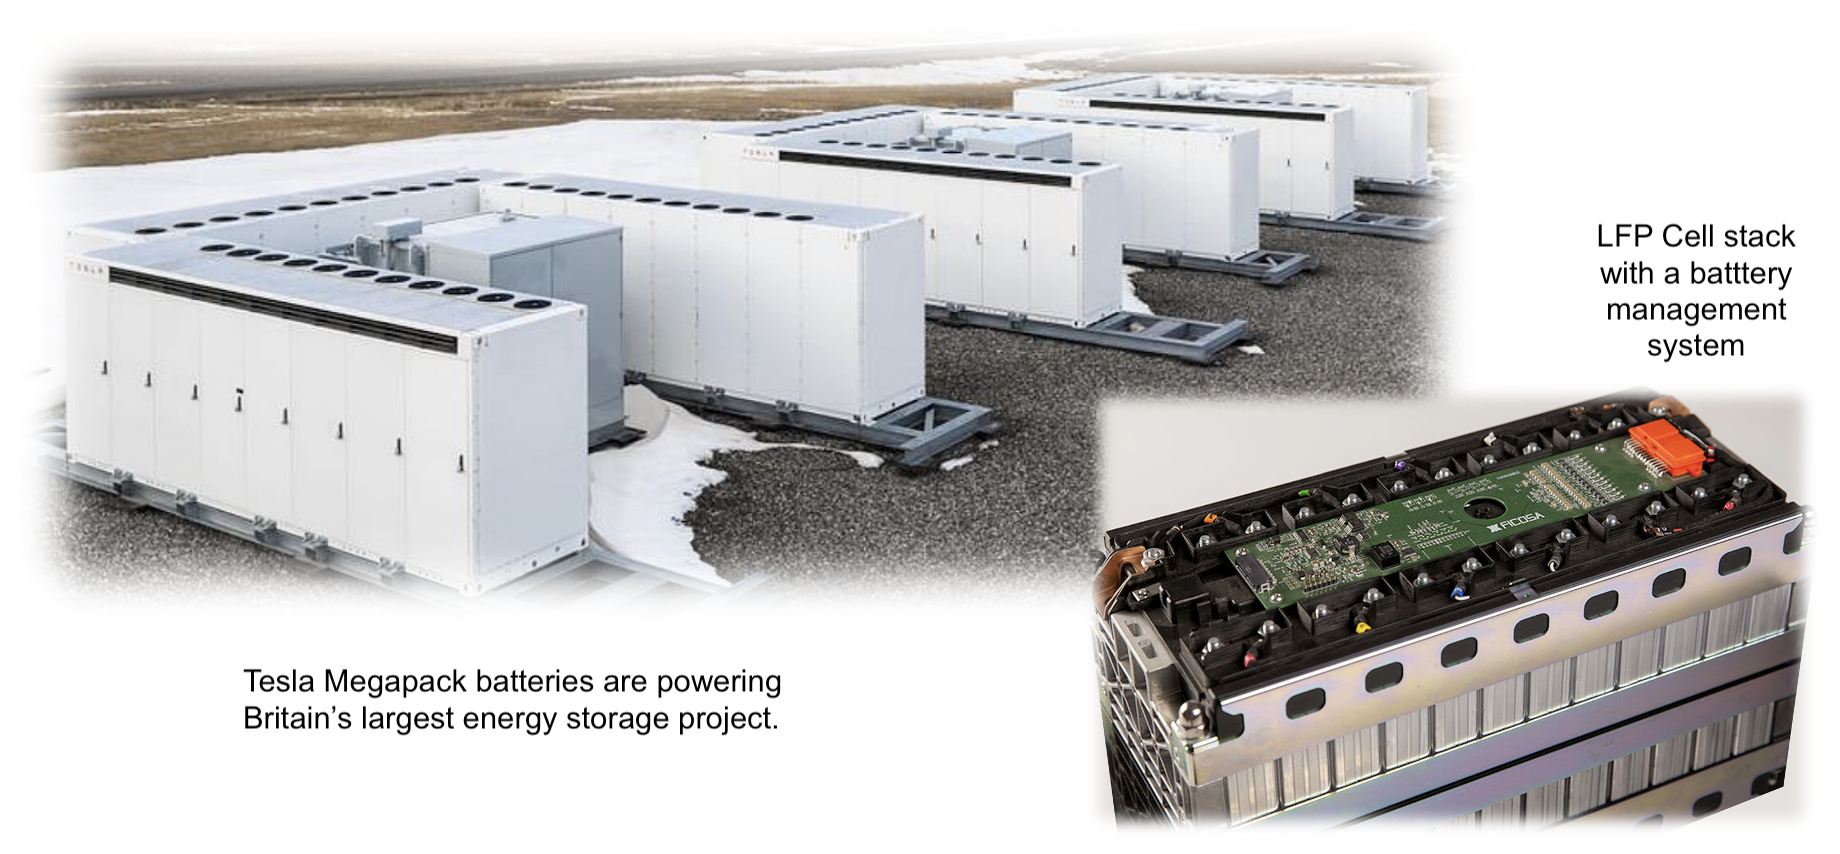
\includegraphics[width=1.0\textwidth]{Skripsie_LaTeXTemplate/Figures/packs.png}
\caption{High Voltage Battery Bank \& a BMS \cite{tessla}}
\label{fig:pak}
\end{figure}
%*****************************************************************************************************%
\section{Problem Statement}\label{sec:probState} %Project motivation: Why do you develop this BMS.
%*****************************************************************************************************%
In the pursuit of developing high voltage battery banks, comprising about 250 cells arranged in series to achieve an approximate voltage of 800V, several significant challenges emerge when interfacing with standard battery management systems (BMS). The primary challenge emanates from the extensive cell strings which, upon connection to a conventional BMS, induce wire overload and inaccurate voltage measurements due to the long wires leading to a single controller, which is ill-suited for precise monitoring across such a vast array of cells.\newline\newline
\noindent
This issue is accentuated by inherent design hurdles associated with high voltage battery banks, such as the imperative need for isolation of communications and transient protection within the BMS to prevent voltage spikes and other transient events, alongside undesirable interactions that could jeopardize system integrity. Accurate state of charge (SOC) and state of health (SOH) estimation of each cell are paramount for safe and efficient battery bank operation.\newline\newline
\noindent
Furthermore, electrical threats like overcurrents, surges, and electrostatic discharge pose additional challenges that the BMS must robustly guard against. The cumulative effect of these challenges elucidates the inadequacy of a single-controller BMS in efficaciously managing and monitoring the numerous cells in high voltage battery banks. Thus, a suitable architecture, that is highly scalable, is desired for the development of high voltage battery banks to overcome the wire overload and inaccurate monitoring predicaments inherent in existing BMS configurations.
%*****************************************************************************************************%
\section{Project Description}\label{sec:projDescrip} %No specific system info or main motivations.
%*****************************************************************************************************%
To address the aforementioned challenges, an innovative design is proposed: deploying a small module with monitoring components and its own micro-controller atop each cell, thereby establishing an individual BMS for each cell. This alternative design significantly mitigates the problem of inaccurate voltage measurements encountered with long wires to a single controller, ensuring a more reliable and robust monitoring system.\newline\newline
\noindent
With voltage measurements taken in close proximity to each cell and facilitated by serial communication between the monitoring modules, a high degree of measurement accuracy is achieved. Initially, the design prototype will be applied to four cells. However, the inherent modular design facilitates seamless scalability, making it adaptable to the high voltage battery bank’s requirements by simply augmenting more cells with modules, fostering a flexible and easily expandable battery management solution.\newpage
\noindent
Although realized through individual module analysis due to logistical and practical constraints, the project's design is fundamentally scalable, allowing for integration into complex, high-voltage systems. The modular BMS, detailed in this report, encompasses hardware design, software development, and performance testing, forming a comprehensive overview of the proposed system.\newline\newline
\noindent
Its modular and adaptable nature guarantees applicability across various domains, positing it as a versatile solution for diverse energy storage requirements, thereby potentially playing a pivotal role in the future energy sector. Through rigorous testing, the superior performance and scalability of the Modular BMS are underscored, demonstrating its potential as a robust and reliable solution for managing Lithium Iron Phosphate (LFP) batteries, and laying a robust foundation for further research and development in battery management technology.
%*****************************************************************************************************%
\section{Report Brief}\label{sec:brief}
%*****************************************************************************************************%
This report presents a detailed review of the project, focusing on the fundamentals of battery management systems and the specifics of the prototype. It covers concepts, design principles, implementation methods, and evaluations, summarizing the project's outcomes and recommendations for future improvements. The flow diagram below provides a structured overview of the report's content.\newline

\begin{figure}[h!]
\centering
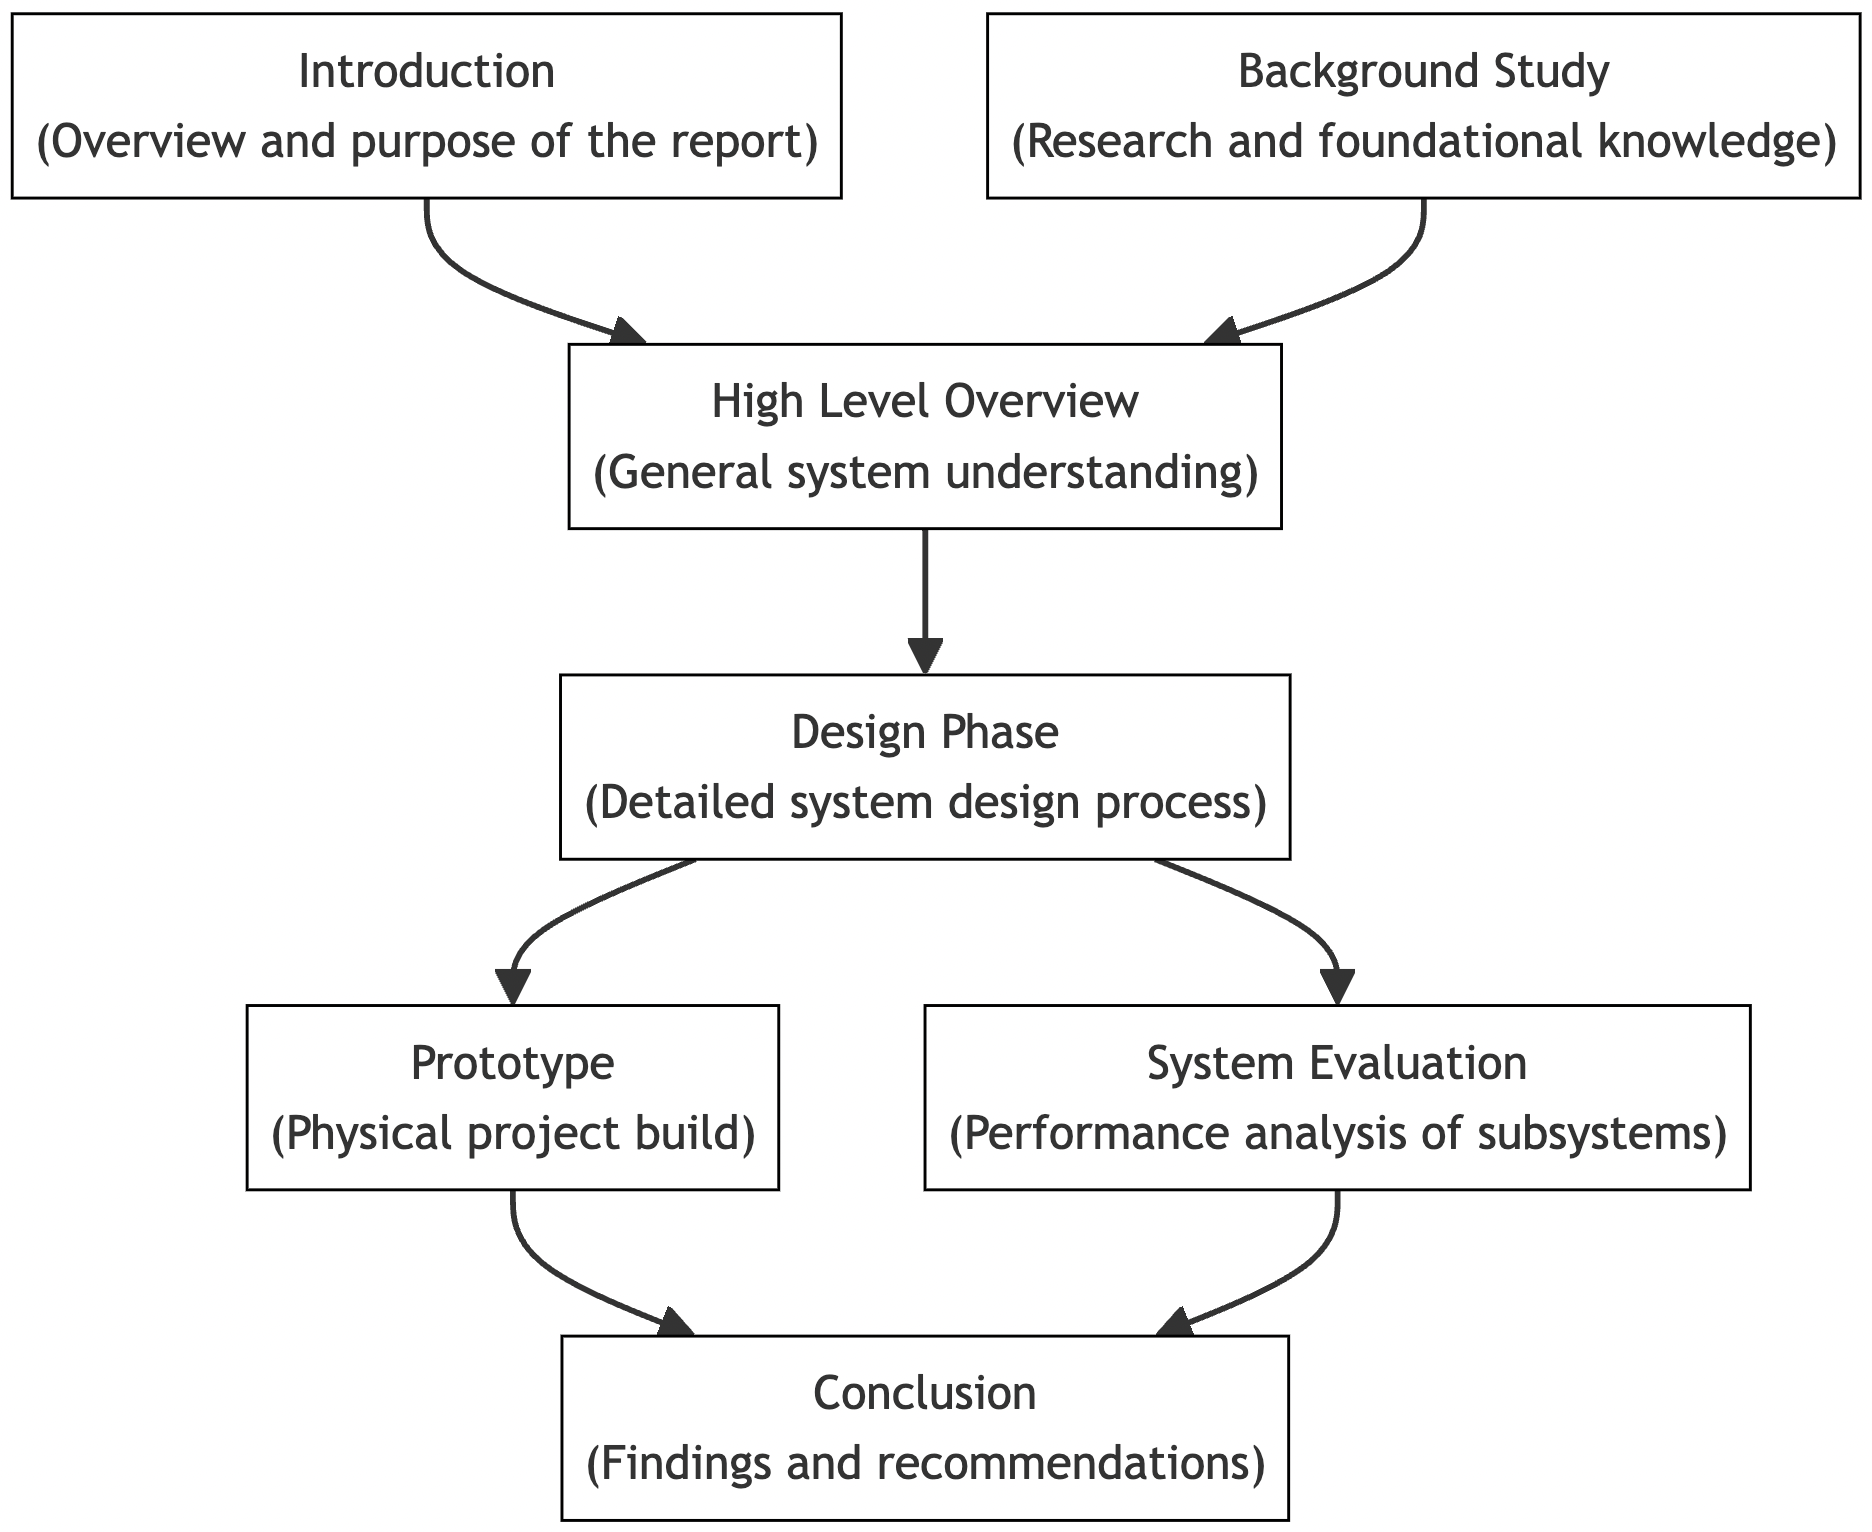
\includegraphics[width=0.7\textwidth]{Skripsie_LaTeXTemplate/Figures/brief.png}
\caption{Report Structured Overview \cite{Mermaid}}
\label{fig:brieff}
\end{figure}

\vfill

\chapter[Background Study]{Chapter 2: Background Study}\label{chap:BG_Study} %Two to three pages long.
%*****************************************************************************************************%
\section{Trending Literature}\label{sec:media1} %BMS Lit of popular media.
%*****************************************************************************************************%
The landscape of battery technology has been rapidly evolving to meet the escalating demands for energy storage solutions, primarily driven by the global transition towards electric vehicles (EVs) and renewable energy. The heart of this evolution lies in the Battery Management Systems (BMS) that ensure safe and efficient operation of batteries, forming a critical component of high voltage battery banks in EVs and grid storage.\newline\newline
\noindent
Recent trends spotlight the shift towards designing scalable modular systems in BMS to accommodate the high voltage requirements. The modular BMS segment, for instance, is projected to register the highest growth rate owing to its ability to connect in series or parallel circuits, thereby augmenting the power/voltage output with the fringe benefit of lower maintenance costs\cite{GlobeNewswire2023}. This indicates a move towards developing flexible and scalable BMS architectures that can seamlessly adapt to varying voltage requirements, essential for high voltage battery banks.\newline\newline
\noindent
In the quest for more affordable and safer electric vehicles, continuous innovation in BMS architectures is pivotal. It's not just about managing existing battery chemistries, but also about being prepared for new and emerging ones. Solid-state batteries, for example, promise more energy in a smaller space, faster charging times, and enhanced safety, which BMS designs need to accommodate\cite{MITTechReview2023}.\newline
\begin{figure}[h!]
\centering
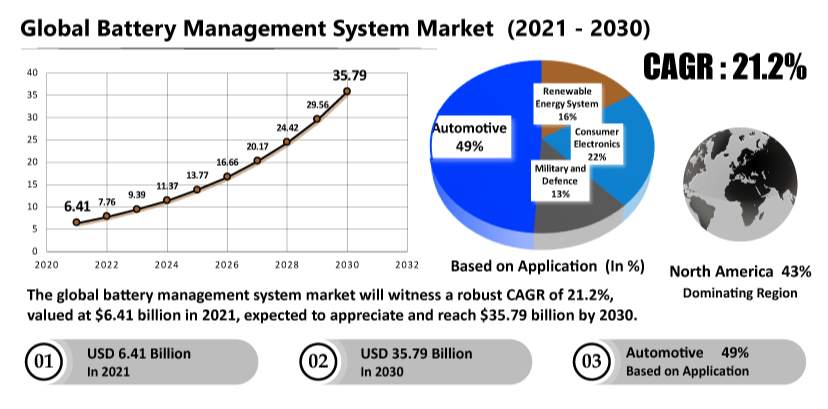
\includegraphics[width=1.0\textwidth]{Skripsie_LaTeXTemplate/Figures/forecast.png}
\caption{Projected Forecast of the BMS Market \cite{m_and_m}}
\label{fig:grow_some}
\end{figure}
\newpage
\noindent
The market's trajectory further corroborates the booming interest in BMS technologies. The global BMS market size, which stood at USD 7.8 billion in 2022, is on a steep ascent, poised to touch USD 55.1 billion, driven by the quest for reducing the cost of battery electronics and simplifying designs to cut down on hardware and wiring costs\cite{BMSSummit2023}.\newline\newline
\noindent
Moreover, the technological advancements by companies like Vitesco Technologies underscore the industry's momentum. With orders worth over 2 billion euros for its innovative BMS, the future seems propitious for further ingenuity in BMS designs, underlining the importance of BMS in the broader narrative of renewable energy solutions\cite{BatteriesNews2023}. This burgeoning sector has caught the attention of various stakeholders, invigorating a flurry of activities around BMS technologies, whether it's about reducing costs, enhancing safety, or accommodating new battery chemistries. As this trend continues, the evolution of BMS is deemed to play a cardinal role in propelling the broader adoption of electric vehicles and renewable energy systems, making it a focal point of interest among industry players, researchers, and policymakers.
%*****************************************************************************************************%
\section{High Voltage DC systems}\label{sec:DC_SYST}
%*****************************************************************************************************%
High voltage DC battery storage systems operate at voltages exceeding 96V, with potential levels up to 384V or even 800V \cite{source1}. With cell modules or individual cells in series, the system achieves the desired operational voltage, each unit incrementing the total voltage. The advantage of high voltage configurations lies in the reduction of $I^{2}\cdot R$ losses, as a higher voltage level lowers the current required for a specific power output, enhancing system efficiency. High voltage systems simplify design by reducing parallel strings and current ratings, lowering component costs and easing battery management, which may enhance reliability and lifespan. To comprehend the simplification for a design, I evaluated examples of HV systems and saw that in principal a design can be formulated using straightforward calculations with equations \ref{eq:HV1}, \ref{eq:HV2} \& \ref{eq:HV3}, adjusting the variables below.\newline

\begin{table}[h]
\centering
\caption{Example Parameters for a HV Battery Bank Design\cite{source2}}
\label{tab:parameters}
\begin{tabular}{|p{7cm}|p{4cm}|p{4cm}|}
\hline
\textbf{Parameter} & \textbf{Symbol} & \textbf{Typical Value} \\ \hline
Nominal voltage of cell/module & \( V_{\text{nom}} \) & 48V \\ \hline
Number of cells/modules in series & \( n \) & Variable \\ \hline
Total System Voltage & \( V_{\text{total}} \) & \( n \cdot V_{\text{nom}} \) \\ \hline
Nominal Capacity & \( C_{\text{nom}} \) & 50Ah \\ \hline
Maximum Charging Current & \( I_{\text{charge}} \) & 50A \\ \hline
Maximum Discharging Current & \( I_{\text{discharge}} \) & 50A \\ \hline
Charge Cut-off Voltage & \( V_{\text{charge,cutoff}} \) & 438V \\ \hline
Discharge Cut-off Voltage & \( V_{\text{discharge,cutoff}} \) & 300V \\ \hline
\end{tabular}
\end{table}
\newpage
\begin{equation}
V_{\text{total}} = n \cdot V_{\text{nom}}
\label{eq:HV1}
\end{equation}
\begin{equation}
C_{\text{total}} = C_{\text{nom}}
\label{eq:HV2}
\end{equation}
\begin{equation}
E_{\text{total}} = V_{\text{total}} \cdot C_{\text{total}}
\label{eq:HV3}
\end{equation}\newline
\noindent
These equations form the basis for designing high voltage battery banks. The modularity of the design allows for scalability; additional modules can be connected in series to increase the voltage or in parallel to increase the capacity, thereby accommodating varying energy storage needs. The operational parameters like maximum charging and discharging currents are crucial to ensure the safety and efficiency of the system.\cite{source3}\newline\newline
\noindent
In summary, the theoretical formulation of a high voltage battery bank hinges on the series connection of cells/modules, with the total system voltage and capacity governed by the nominal voltage and capacity of individual cells/modules. This modular and scalable design is fundamental to meeting the diverse energy storage requirements across different applications.
%*****************************************************************************************************%
\section{Lithium Ferro Phosphate Technology}\label{sec:LFP}
%*****************************************************************************************************%
\textbf{\emph{Chemistry of LFP Cells}}\newline
\noindent
Lithium Iron Phosphate (LiFePO4 or LFP) cells function through the process of lithium ions moving from the cathode to the anode and vice versa during discharge and charge cycles, respectively. This movement, termed intercalation (insertion) during discharge and deintercalation (extraction) during charge, facilitates the storage and release of electrical energy. The primary components of an LFP cell are its cathode, composed of lithium iron phosphate, its anode made of graphite, and the electrolyte, a lithium salt dissolved in an organic solvent. The cathode serves as the source and sink of lithium ions, enabling the reversible electrochemical reactions crucial for the cell's energy storage and delivery.\cite{LiFePO4Wiki}\newline\newline
\noindent
$Discharge$
\[ \text{Cathode: } \text{LiFePO}_4 \rightarrow \text{FePO}_4 + \text{Li}^+ + e^- \]
\[ \text{Anode: } \text{LiC}_6 + \text{Li}^+ + e^- \rightarrow 6\text{C} \]
$Charge$
\[ \text{Cathode: } \text{FePO}_4 + \text{Li}^+ + e^- \rightarrow \text{LiFePO}_4 \]
\[ \text{Anode: } 6\text{C} \rightarrow \text{LiC}_6 \]
\newpage
\noindent
\textbf{\emph{Typical Data Specs}}\newline
\noindent
- \emph{Nominal Voltage}: $3.2V$\newline
- \emph{Energy Density}: $90 Wh/kg$ - $120 Wh/kg$\newline
- \emph{Cycle Life}: $>2000$ cycles ($80\%$ DoD)\newline
- \emph{Charge/Discharge Efficiency}: $95\%$ - $98\%$\newline
- \emph{Operating Temperature Range}: $-20^{o}C$ to $60^{o}C$\newline\newline
\noindent
\textbf{\emph{C Rating}}\newline
\noindent
The C rate denotes the rate at which a battery is charged or discharged, calculated as:
\[ \text{C Rate} = \frac{\text{Current (A)}}{\text{Capacity (Ah)}} \]
\noindent
\textbf{\emph{Discharge Current}}\newline
\noindent
For a 100Ah cell with a 1C rate, the current capability for 1 hour of constant discharge is:
\[ \text{Current (A)} = \text{C Rate} \times \text{Capacity (Ah)} = 100A \]
\noindent
\textbf{\emph{Charge Current}}\newline
\noindent
Selection of charge current, guided by manufacturer specifications, affects charging time, heat generation, and cell lifespan.\newline\newline
\noindent
\textbf{\emph{Cells in Series}}\newline
\noindent
In series connections, voltage accumulates while capacity remains constant, necessitating careful management to prevent overcharge or over-discharge.\newline\newline
\noindent
\textbf{\emph{Cell Balancing}}\newline
\noindent
Balancing ensures equal state of charge (SoC) in series-connected cells, employing active or passive techniques to prevent overcharge or over-discharge.\newline\newline
\noindent
\textbf{\emph{Cell Comparison}}
\begin{table}[h]
    \centering
    \caption{Cell Types \cite{cell_COMP1}\cite{cell_COMP2}}
    \label{tab:cell_comparison}
    \begin{tabular}{|p{2.7cm}|p{3.8cm}|p{3.8cm}|p{3.8cm}|}
        \hline
        Aspect & LFP (LiFePO4) & NMC (LiNiMnCoO2) & LCO (LiCoO2) \\
        \hline
        Energy Density & $\sim$90-120 Wh/kg & $\sim$150-220 Wh/kg & $\sim$200 Wh/kg \\
        \hline
        Safety & Higher & Lower & Lower \\
        \hline
        Lifespan & $>$2000 cycles & $\sim$1000-2000 cycles & $\sim$500-1000 cycles \\
        \hline
        Cost & Less Expensive & More Expensive & Expensive \\
        \hline
        Thermal Range & -20°C to 60°C (-4°F to 140°F) & -20°C to 55°C (-4°F to 131°F) & -40°C to 70°C (-40°F to 158°F) \\
        \hline
        Industry Usage & $31\%$ & N/A & N/A \\
        \hline
    \end{tabular}
\end{table}

\newpage
%*******************************************%
\section{Battery Cell Monitor and Control}\label{sec:Cell_M}
%*******************************************%
\subsubsection{Battery Management}\label{subsec:BM}
Battery management is pivotal to the evolution and efficiency of battery-operated systems, marking a significant stride from the invention of the first true battery by Alessandro Volta in 1799, to the modern rechargeable batteries pioneered by Gaston Plante in 1859\cite{1}. The burgeoning rise of electric vehicles (EVs) and the global shift towards carbon neutrality underscored the imperative for adept battery performance monitoring and management for enhanced efficiency, safety, and user satisfaction\cite{2}.\newline\newline
\noindent
Historically, the nascent forms of battery management were rudimentary, primarily encompassing basic protection circuits for discharge current tripping, which were unstable. The evolution of electronic protection circuits, integrated into comprehensive battery management systems (BMS), marked a significant advancement, catering to a myriad of battery chemistries\cite{3}. Passive cell balancing emerged as a technique to equalize the State of Charge (SoC) among cells in a battery stack, particularly focusing on cells with lower capacity to ensure balanced performance\cite{4}.\newline\newline
\noindent
With the proliferation of onboard batteries across various applications, the exigency for advanced management burgeoned, precipitating the development of centralized and distributed battery management systems aimed at bolstering battery performance and user experiences\cite{5}. The evolution of batteries was inextricably tied to the products and systems that employed them. The burgeoning demand for improved portable power sources, propelled by the ubiquity of mobile computing and communication, spearheaded innovations in battery management technology\cite{6}.
\subsubsection{Controller Topology}\label{subsec:CnTp}
The controller topologies in Battery Management Systems (BMS) are quintessential for efficient monitoring and regulation of battery packs. These topologies are crafted to meet specific requirements and applications, thereby ensuring the safety and reliability of battery operations.\newline\newline
\noindent
\emph{Centralized Topology:}\newline
\noindent
In a centralized topology, a singular control unit is interfaced with each cell in the battery pack through separate wiring. This control unit is pivotal for monitoring and managing the battery cell parameters, thereby ensuring the safe and reliable operation of the overall battery pack\cite{7}.\newline\newline
\noindent
\emph{Modular Topology:}\newline
\noindent
The modular topology encompasses a master controller, multiple slave controllers, and an electric meter. The master controller orchestrates communication with the slave controllers, each accountable for a subset of battery cells, while the electric meter furnishes pack-level readings. This topology is employed to manage larger battery packs efficiently, offering a scalable solution for battery management\cite{8}.\newline\newline
\noindent
\emph{Distributed Topology:}\newline
\noindent
In a distributed topology, dedicated control units are allocated at a central control unit, each tethered to individual battery cells. This setup facilitates granular control and monitoring of each cell, ensuring swift identification and rectification of any discrepancies in cell performance. Although the control units are dedicated, they are centrally located, not positioned atop each cell, which augments the monitoring efficacy while maintaining a structured control hierarchy\cite{9}.\newline\newline
\noindent
The choice of topology is contingent on the application, size, and configuration of the battery pack, and the requisite level of control and monitoring. The broad spectrum of applications with different voltage classes, necessitates divergent controller topologies to align with the hardware requirements of BMS for a given application. Understanding these topologies and their ramifications on the BMS performance is instrumental for engineers to design and implement efficacious and reliable BMS controllers.
%*******************************************%
\section{Module Communication Methodology}\label{sec:commsMeth}
%*******************************************%
Communication is crucial for the effective functionality of the envisioned system, as it facilitates the transfer of data and enables interaction between individual cells through their respective monitoring modules. A comprehensive investigation was undertaken to discern a communication methodology that aligns seamlessly with the project's overarching objectives. Initial evaluations delved into the Canbus design orchestrated by Stuart Pittaway\cite{stuart_pittaway} and the isoSPI design conceived by Mark Wolf\cite{mark_wolf}, yet both methodologies were deemed incompatible with the project's requirements. Subsequently, the isolated UART serial communication design emerged as a suitable solution, rendering compatibility with the smaller microcontrollers envisaged for the project, and permitting isolation between differing voltage levels across the communication pathway, ensuring a robust communication framework\cite{TIDA00163}.\newline\newline
\noindent
Two principal communication configurations were meticulously explored: the daisy-chain and all-call UART connection configurations, as illustrated in Figures \ref{fig:daisy} and \ref{fig:allcall}, respectively. The daisy-chain configuration links devices in a series, each connected to the next device's RX and TX pins, forming a closed loop, as further elucidated by a reference design from Texas Instruments specifically tailored for battery management applications\cite{TI_UART_SPI_bridgee}. On the other hand, the all-call configuration establishes a parallel connection of devices to a single communication line, with all devices interfacing directly with the master controller's RX and TX pins, thereby centralizing the communication system.

\begin{figure}[!htb]
\centering
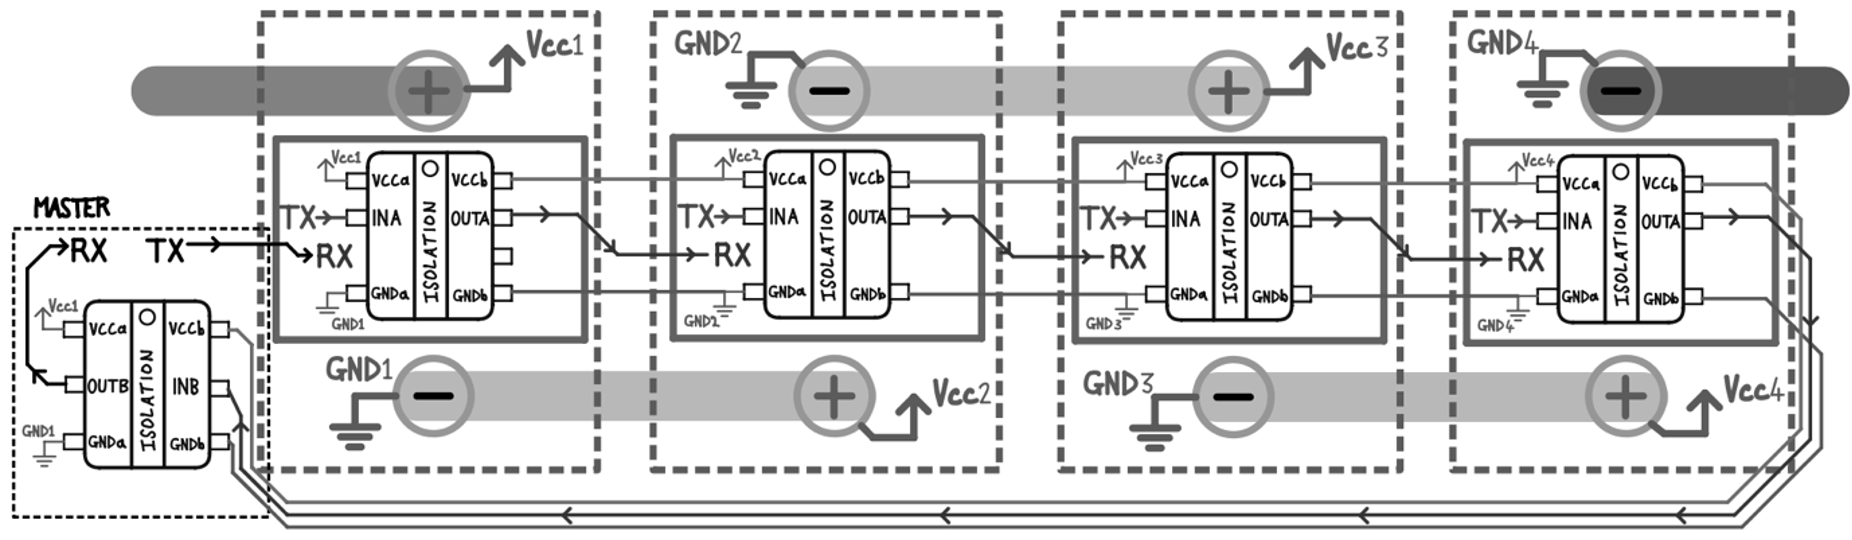
\includegraphics[width=1.0\linewidth]{Figures/DaisyChain.png}
\caption{Daisy-chain configuration.}
\label{fig:daisy}
\end{figure}
\noindent
The depicted diagram above illustrates a daisy-chain architecture among a stack of microcontrollers, where each device transmits messages sequentially, initiating a new cycle upon completion of the loop. Each device in the chain transmits only after successful reception. This allows the modules to receive messages from the other modules within one full cycle.

\begin{figure}[!htb]
\centering
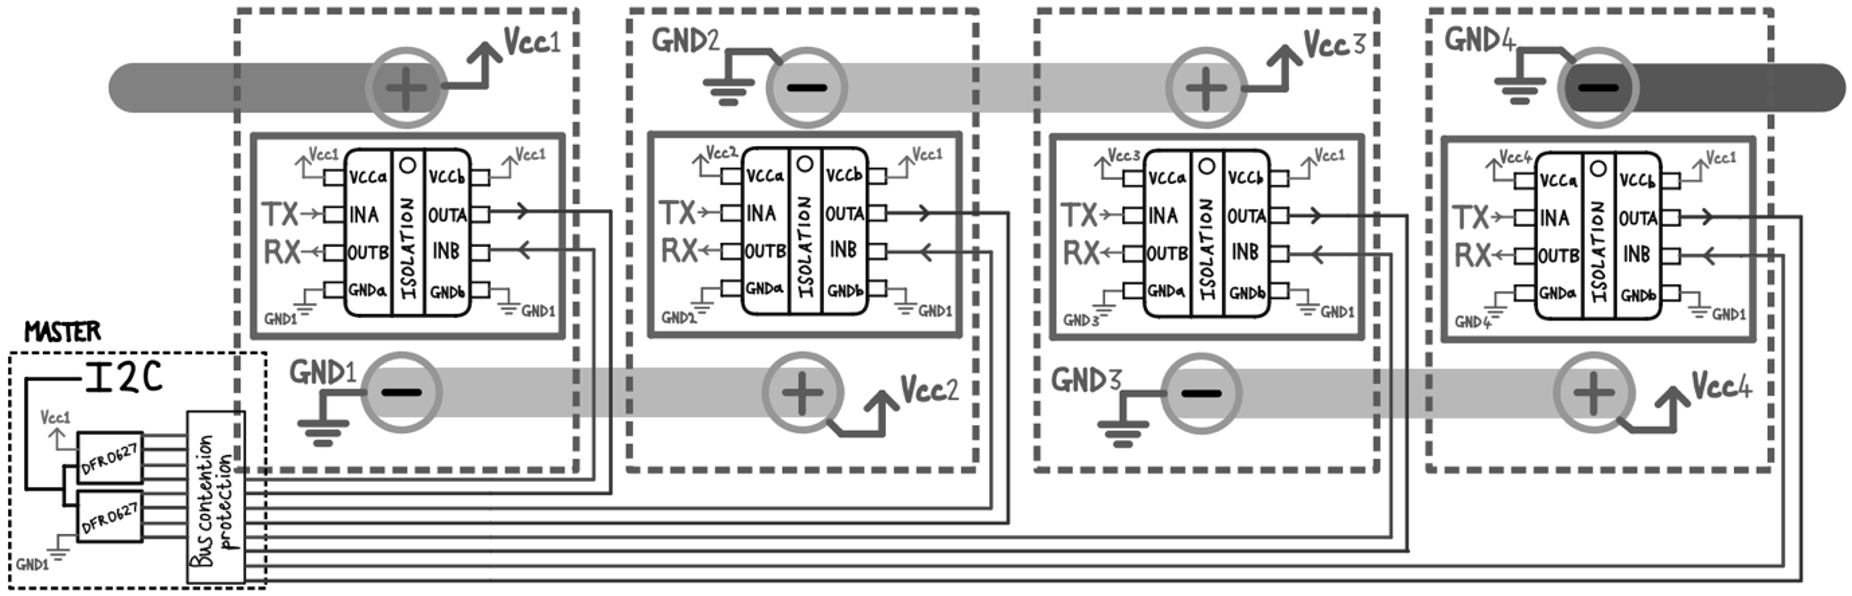
\includegraphics[width=1.0\linewidth]{Figures/AllCall.png}
\caption{All-call configuration.}
\label{fig:allcall}
\end{figure}
\noindent
In the all-call configuration, modules communicate exclusively with the main controller, which operates in parallel with the slave modules. System data exchange among all modules now necessitates two cycles, albeit expedited due to the main controller's broadcast capability.\newline\newline
\noindent
A comparative analysis of these configurations is presented in Table \ref{tab:UART_comparison}, delineating various aspects like hardware and wiring complexity, transmission delay, data rate, software complexity, and fault tolerance.
\newpage
\begin{table}[h]
\centering
\caption{UART Hardware Configuration Comparison}
\label{tab:UART_comparison}
\begin{tabular}{|p{2.2cm}|p{6.1cm}|p{7cm}|}
\hline
\textbf{Feature} & \textbf{Daisy-Chain Configuration} & \textbf{Bus Configuration} \\
\hline
Definition & Devices are connected in a series, with each device connected to the next device's RX and TX pins, forming a closed loop & Devices are connected in parallel to a single communication line, with all devices connected to the same RX and TX pins of the master controller \\
\hline
Hardware Complexity & Simple, each device requires only two connections for RX and TX & More complex, requires additional hardware components, such as pull-up resistors and line drivers, to ensure reliable communication \\
\hline
Wiring Complexity & Increases with the number of devices in the chain, requires more connections between devices & Simplifies wiring, reduces number of connections required, all devices are connected to the same lines \\
\hline
Transmission Delay & Each device must wait for the previous device to complete its transmission before transmitting data, limiting the data rate & Devices can transmit data at any time, without waiting for other devices, potentially increasing the data rate \\
\hline
Data Rate & Limited by the transmission delay between devices, which increases with the number of devices in the chain & Potentially higher, depending on hardware and software design, can support higher data rates \\ 
\hline
$DataRate_{MAX}$ & $DR_{max} = \frac{baudrate\times(\#data bits per byte)}{10\times(\#devices)}$ & $DR_{max} = \frac{baudrate}{10\times(\#data bits + parity bits + stop bits)}$ \\ 
\hline
Software Complexity & Higher, requires time delay programming for each device to ensure data is transmitted in sequence & Simpler, devices can transmit data at any time, without waiting for other devices \\
\hline
Fault\newline Tolerance & Communication can be disrupted if any device fails, since it breaks the closed loop & Communication can continue as long as at least one device remains functional, since all devices are connected in parallel \\
\hline
Advantages & Simple hardware design, suitable for small-scale systems with a few devices & Simplifies wiring, can support higher data rates, suitable for larger systems with multiple devices \\
\hline
Drawbacks & Limited data rate, requires time delay programming for each device, may be disrupted if any device fails & More complex hardware design, requires additional components, may be more expensive, may require higher software complexity to manage communication \\
\hline
\end{tabular}
\end{table}

\noindent
Based on the analysis, a hybrid solution amalgamating elements from both configurations was devised. This hybrid solution encapsulates the communication methodology aimed for this project, offering a balance of simplicity, reliability, and scalability. More discussion on the communication system and its detailed hardware design is done in section \ref{subsubsec:iso_COMS}, where the diagram for the hybrid solution is also presented in Figure \ref{fig:MM_D2}.
%*******************************************%


\vfill

\chapter[High Level Overview]{Chapter 3: High Level Overview}\label{chap:HL_overview}
%*******************************************%
\section{Summary}\label{sec:intro_HLovv}
This chapter offers a high-level overview of the project. The "Concept Investigation" section explores the methodology underpinning the project's core idea. The "Design Requirements" section outlines critical specifications and constraints guiding the design. The "Scalable Architecture" section examines the design's adaptability to varying scales and configurations. Lastly, the "Hypothesis \& Potential Drawbacks" section discusses assumptions and possible challenges encountered in the design process.
%*******************************************%
\section{Concept Investigation}\label{sec:consep}
%*******************************************%
The mainstream approach towards Battery Management Systems (BMS) for large battery banks in the industry has traditionally hinged on robust BMS controllers adept at managing long series cell strings. These systems are generally designed with a fixed cell management capacity, thereby lacking inherent scalability. The prevalent paradigm encapsulates a fixed number of cells within a module, each equipped with its dedicated BMS. These modules can then be arranged in series, with each BMS capable of inter-module communication, facilitating a level of scalability as depicted in the following diagram:

\begin{figure}[h!]
\centering
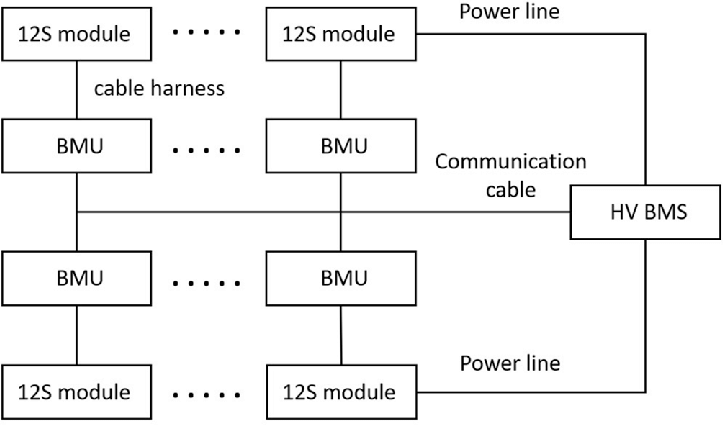
\includegraphics[width=0.4\textwidth]{Skripsie_LaTeXTemplate/Figures/HV_BANK_diaaa.png}
\caption{Conventional BMS approach for a high voltage battery bank\cite{generic}}
\label{fig:Conventional}
\end{figure}
\noindent
However, this conventional methodology manifests certain limitations upon scaling, primarily due to the introduction of inaccurate measurements and control constraints. The inaccuracies might stem from the cumulative error propagation and latency in communication as the number of series-connected modules escalates. Moreover, the fixed design poses a barrier to seamless scalability and flexibility in system expansion.\newline\newline
\noindent
To transcend these limitations and achieve enhanced accuracy in cell monitoring, a novel concept is proposed. Rather than modularizing a group of cells with a shared BMS, each cell is envisioned to be accompanied by its individual monitoring system. The core of this innovative design lies in stacking cells each endowed with its own monitoring system, thereby circumventing the scalability constraints imposed by traditional designs. The scalability in this scenario is principally governed by the communication bandwidth and line impedance between the monitoring systems.\newline\newline
\noindent
The proposed design envisages a miniature module atop each cell, housing monitoring components and a dedicated micro-controller, thereby rendering an individualized BMS for every cell. While the prototype is tailored for four cells, the intrinsic design flexibility enables scaling up to accommodate high voltage battery banks by merely augmenting the system with additional cells and modules.\newline\newline
\noindent
This modular BMS design essentially mirrors the architecture of a conventional BMS but miniaturizes it to fit atop each cell independently. Consequently, every cell in the series string is furnished with a parallel-connected monitoring module. Each of these modules, equipped with its micro-controller, is tasked with processing measurements and relaying the data to a central master device for either storage or further dissemination. The interconnection among all boards facilitates seamless communication, thereby fostering a comprehensive understanding of the battery pack's state across all modules. This collective insight empowers each module to evaluate the global state of the battery pack and fine-tune its respective cell’s variables accordingly. The following diagram elucidates the conceptual design of this novel BMS architecture:

\begin{figure}[h!]
\centering
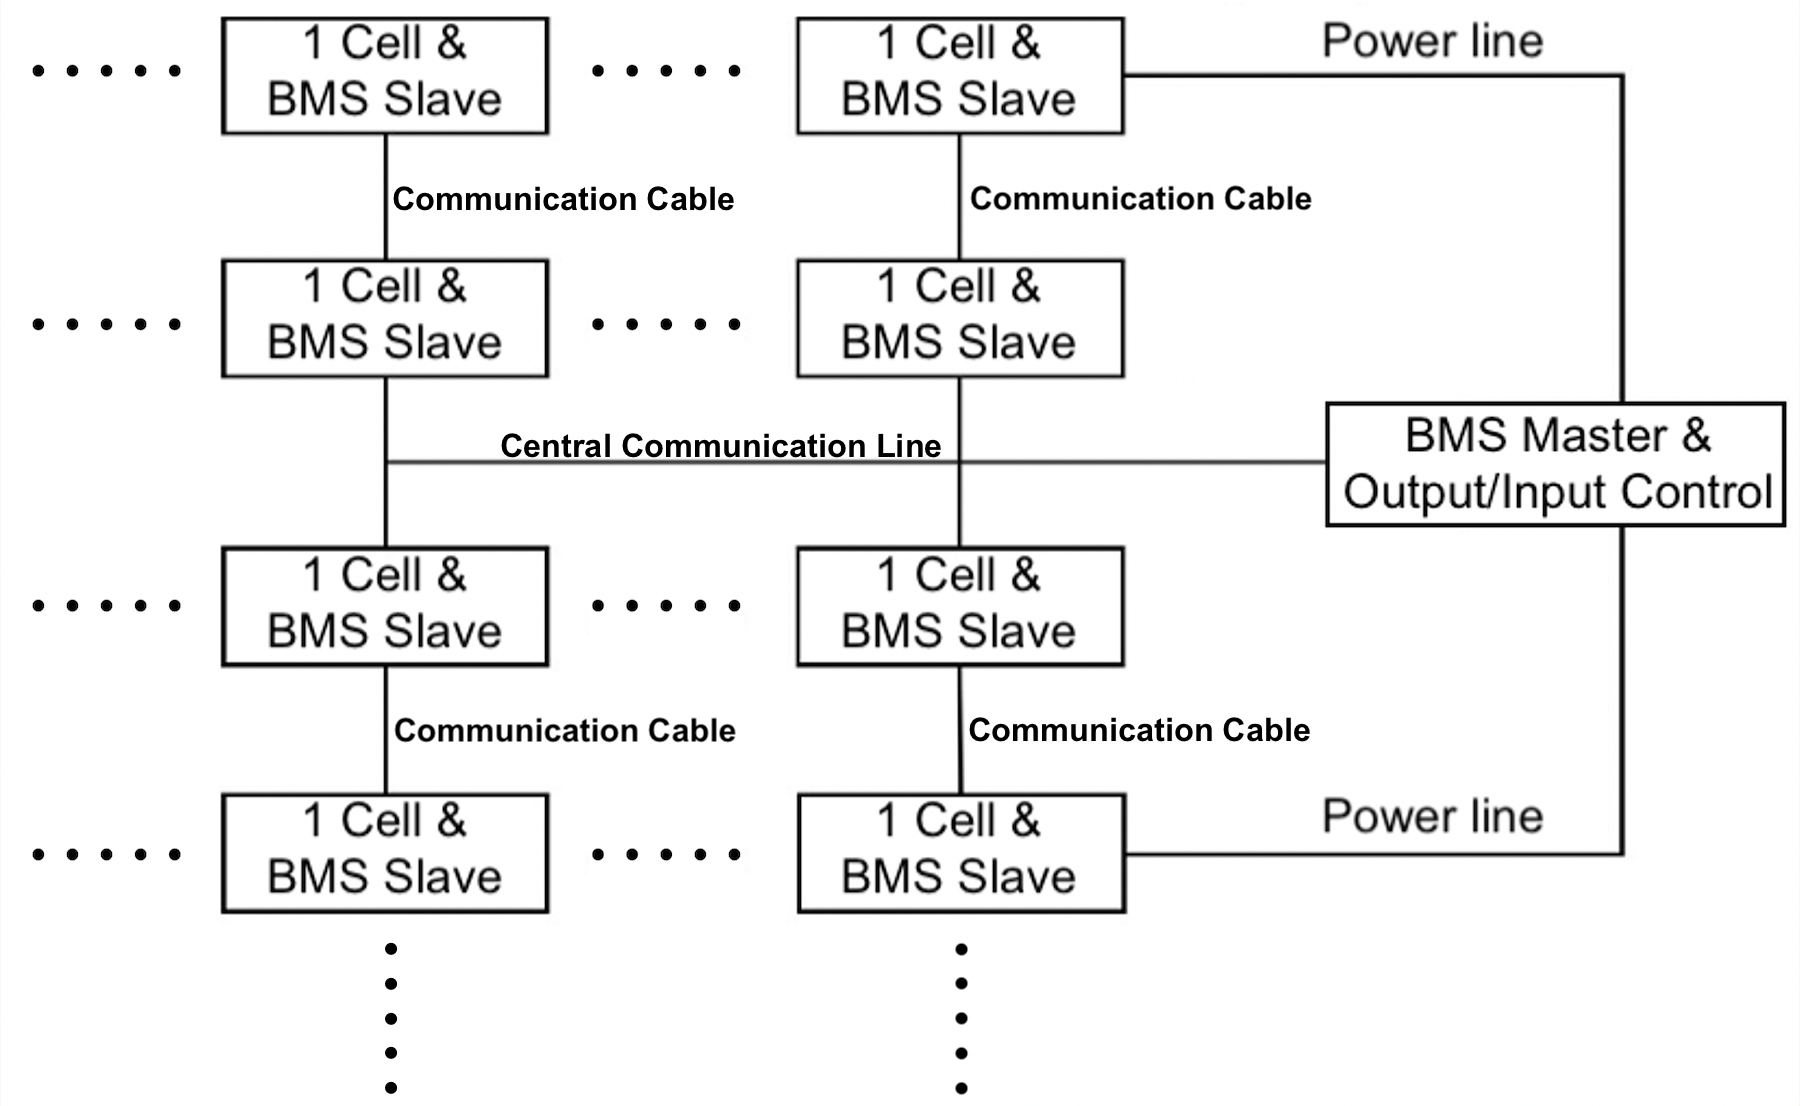
\includegraphics[width=0.5\textwidth]{Skripsie_LaTeXTemplate/Figures/NEW_HV_BANK_diaaa.png}
\caption{Concept Design for a modular BMS}
\label{fig:Conventional1}
\end{figure}
%*******************************************%
\section{Design Requirements}\label{sec:DesignReq}
%*******************************************%
The concept design investigated above will be developed in the hardware design of the system to meet requisites for the Battery Management System (BMS) aimed at ensuring modularity, scalability, and reliable performance.

\begin{itemize}
    \item \textbf{Modularity and Scalability}: The BMS is designed to independently monitor an extendable number of cells through dedicated subsystems for each cell. The initial prototype will monitor four cells, with scalability being a core attribute to accommodate a potentially indefinite number of cells.
    
    \item \textbf{Communication}: Serial communication via Universal Asynchronous Receiver/Transmitter (UART) protocol will be established among cell monitoring modules and between the modules and the master controller. Isolation in communication is required to handle different voltage levels across the string of cells.
    
    \item \textbf{Safety Features}: Essential safety features include cell temperature monitoring, cell voltage monitoring, cell balancing, string current monitoring, a reliable relay disconnect mechanism for anomaly detection, force reset functionality for non-responsive scenarios, and over-current protection facilitated through fuses.
    
    \item \textbf{Cell Monitoring}: Optimized for 105 Ah LFP cells, the design targets maintaining cell terminal voltage within 3.35V to 3V for operational longevity. Accurate voltage monitoring is required, with a preliminary accuracy of around ±0.05\%. Although cell temperature monitoring does not necessitate high accuracy, exceptional reliability is mandatory.
    
    \item \textbf{Cell Balancing}: Passive balancing will be employed, with each monitoring module hosting a dedicated dump load circuit targeting a balancing current of around 1A per cell, aligning with the good practice of 1\% of the cell's current capacity.
    
    \item \textbf{Power Supply}: Cell monitoring modules will be powered individually by the respective cells they are monitoring, with cell voltage boosted to a constant 5V for logic level optimization. The master controller will be powered from the series string of four cells through a buck supply delivering 5V.
    
    \item \textbf{Physical Constraints}: The monitoring modules' PCB dimensions are constrained to approximately 40mm x 40mm to fit between the cell terminals and edges of the cell.
    
    \item \textbf{Data Rate}: While there is no specific requirement for the data rate, a fairly fast rate is desired. The precise data rate will be determined during the serial communication design phase, and data integrity assurance is not a priority as the design will be used prototype-based.
\end{itemize}
%*******************************************%
\section{Scalable Architecture}\label{sec:scale_HLovv}
%*******************************************%
The proposed BMS architecture employs individual cell monitoring modules in parallel with each cell in a battery bank, addressing key scalability issues:

\begin{enumerate}
    \item \textbf{Wiring Complexity}: Utilizes four short wires per module for communication and cell terminal connections, minimizing wiring harness and failure risks.
    \item \textbf{Switching and Sizing}: Independent monitoring and dedicated balancing load per module ensure precise switching and optimal sizing.
    \item \textbf{Single-Cell Focus}: Individualized monitoring eliminates multicell complications, with inter-module communication ensuring coherent system understanding.
    \item \textbf{Scalable BMS Architecture Pathway}: The modular design inherently scales with battery bank expansion, promoting a seamless, scalable BMS architecture.
\end{enumerate}
\noindent
This architecture significantly mitigates conventional scalability challenges, warranting further research and development for efficient, scalable BMS solutions.
%*******************************************%
\section{Hypothesis \& Potential Drawbacks}\label{sec:drawbacks}
%*******************************************%
This project aims to advance high voltage battery management system (BMS) innovations by designing and evaluating a modular cell monitoring system. The goal is to explore a novel BMS architecture that could inspire future models and enhance the management of LFP cells at high voltages. Although the initial design iteration may not be ready for real-world application, it will provide a foundation for understanding the principles and configurations fundamental to a modular BMS for LFP batteries. The initial phase will focus on experimental design and analysis.\newline\newline
\noindent
The development will involve a comprehensive process of design and conceptualization to establish a foundational evaluation framework. Given the complex nature of electronic design, encountering unforeseen challenges is expected and listing all potential drawbacks would be impractical. The project's scope may expand due to its multidimensional nature, necessitating strict adherence to a research, design, develop, and evaluate cycle to maintain focus. The timeline is structured to permit only a single design iteration, provided there are no deviations from the planned path.\newline\newline
\noindent
Component availability and procurement delays are anticipated to affect the schedule, potentially compressing the time available for evaluation. Given the project's scale and timeframe, debugging and design reviews will likely proceed in parallel. Strategies to mitigate time delays include task overlapping, which aims to streamline the project's workflow and minimize disruptions.
%*******************************************%




\vfill

\chapter[Detailed Design]{Chapter 4: Detailed Design}\label{chap:hard_dsgn}%This chapter must be a lot of pages.
%*******************************************%
\section{Introduction}\label{sec:intro_dsgn}
%*******************************************%
In this chapter, we delve into the comprehensive design process for the proposed scalable modular Battery Management System. Initially, the design processes for the independent monitoring modules and the main controller are explored separately. Subsequently, the communication system combines the designs of these entities as the main controller serves to collect and process the data monitored by the cell modules. The systematic approach for the design process entails the circuit designs, component selection, and the printed circuit board layout. Afterwards a merged design review of the system is done.
%*******************************************%
\section{System Overview}\label{subsec:syst_OVV}
%########################################################
As illustrated in figure \ref{fig:ovvv_dsgn} below the modular BMS design essentially has the same setup as a traditional BMS but the whole system is fitted to each cell independently. As a result, every cell in the series string is equipped with a monitoring module connected in parallel, enabling us to acquire more accurate and precise measurements from each cell. These modules feature their own microcontroller, responsible for processing the measurements and transferring the data to a master device for storage or sharing. Additionally, all the boards are interconnected, allowing for seamless communication and establishing a global view of the battery pack. This collective understanding enables each module to assess the state of the entire pack and make necessary adjustments to its respective cell’s variables.

\begin{figure}[h!]
\centering
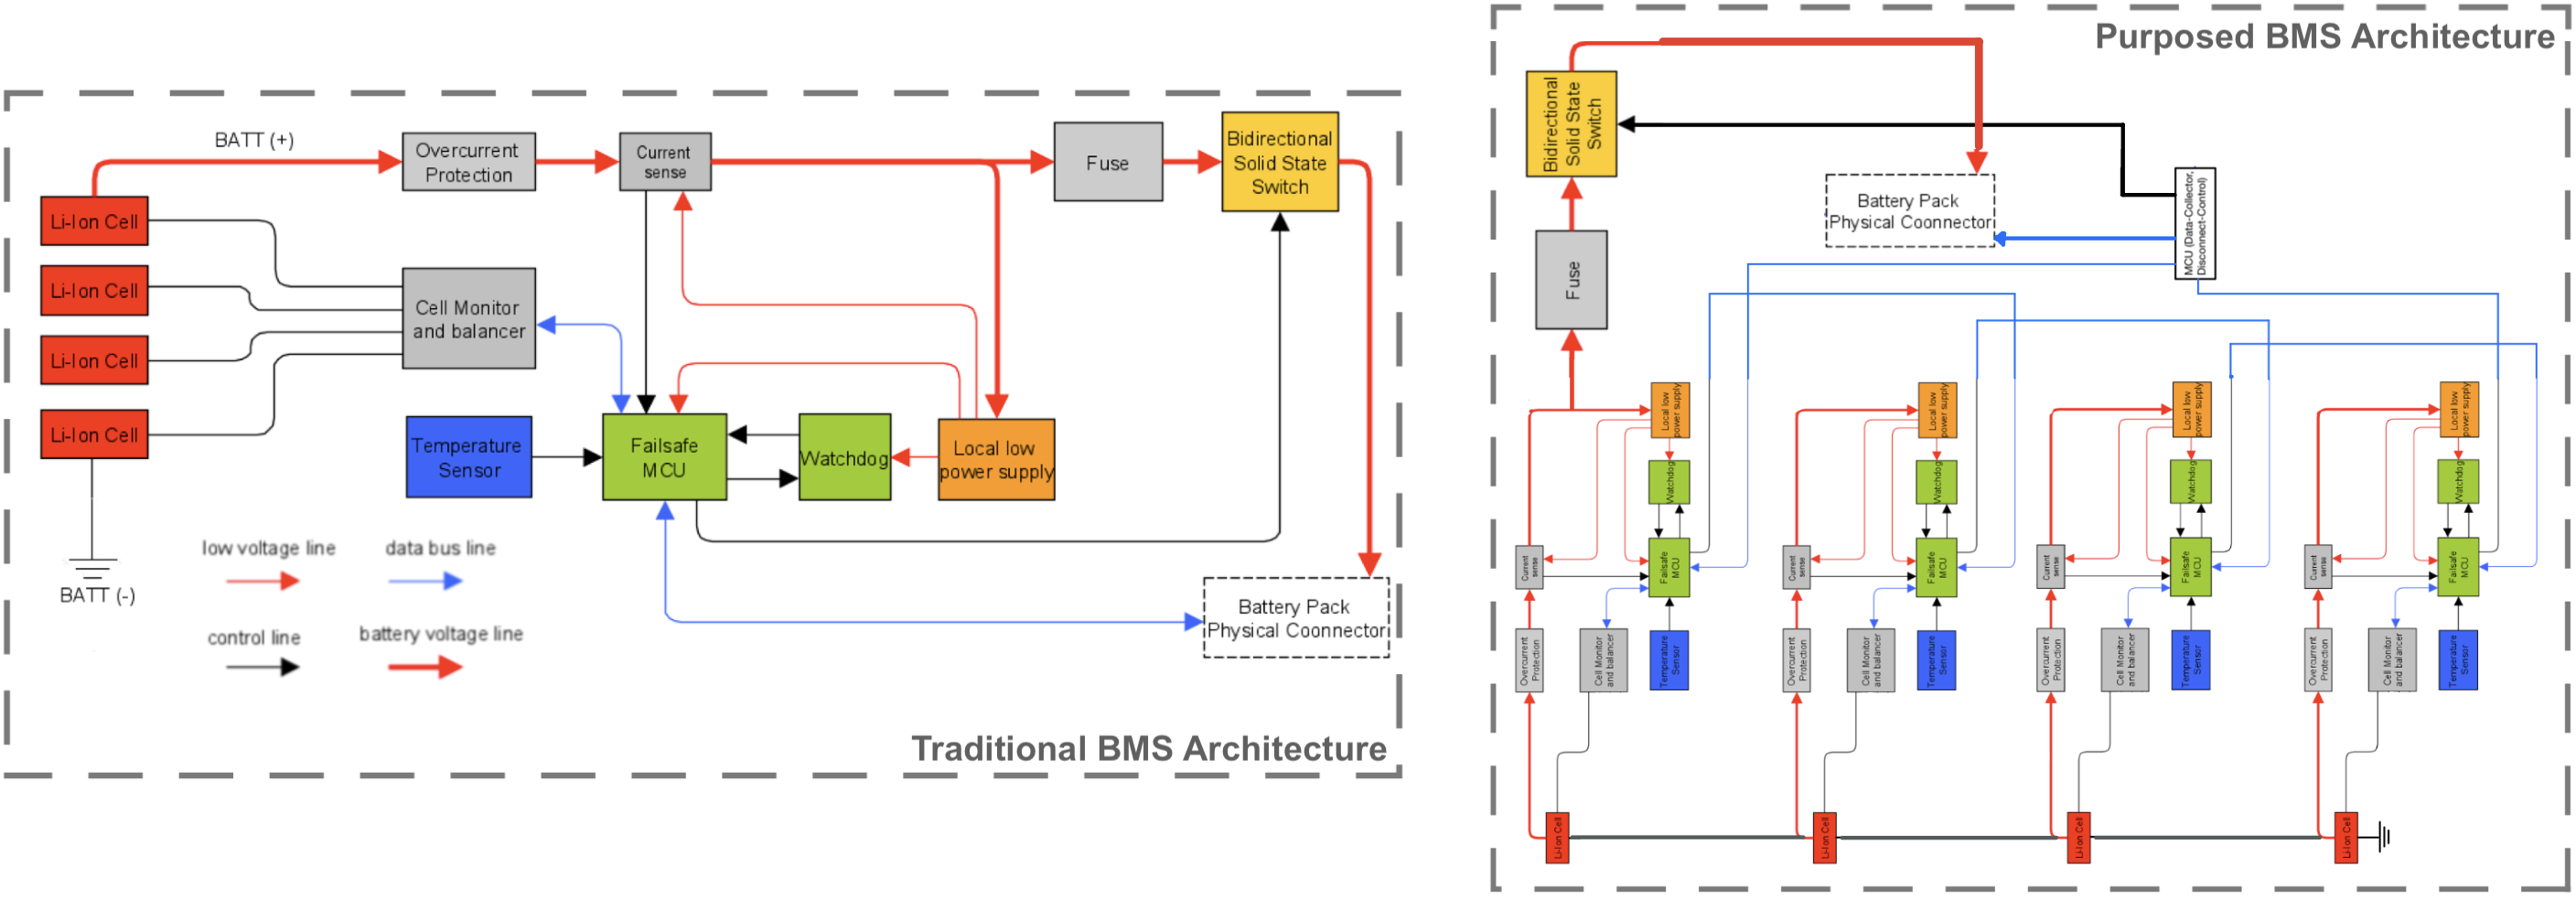
\includegraphics[width=0.9\textwidth]{Skripsie_LaTeXTemplate/Figures/simpleBMS_Diagram.png}
\caption{Envisioned Architecture of the Proposed BMS}
\label{fig:ovvv_dsgn}
\end{figure}

\noindent
The BMS monitoring boards will be attached to each cell in the battery pack. Their sole wired connection will be the communication line linking the cells, which significantly reduces the use of extensive wiring in the system. The primary (master) controller, located externally, interfaces with the battery pack and facilitates connections to either the load or charger.
\newpage
\begin{figure}[h!]
\centering
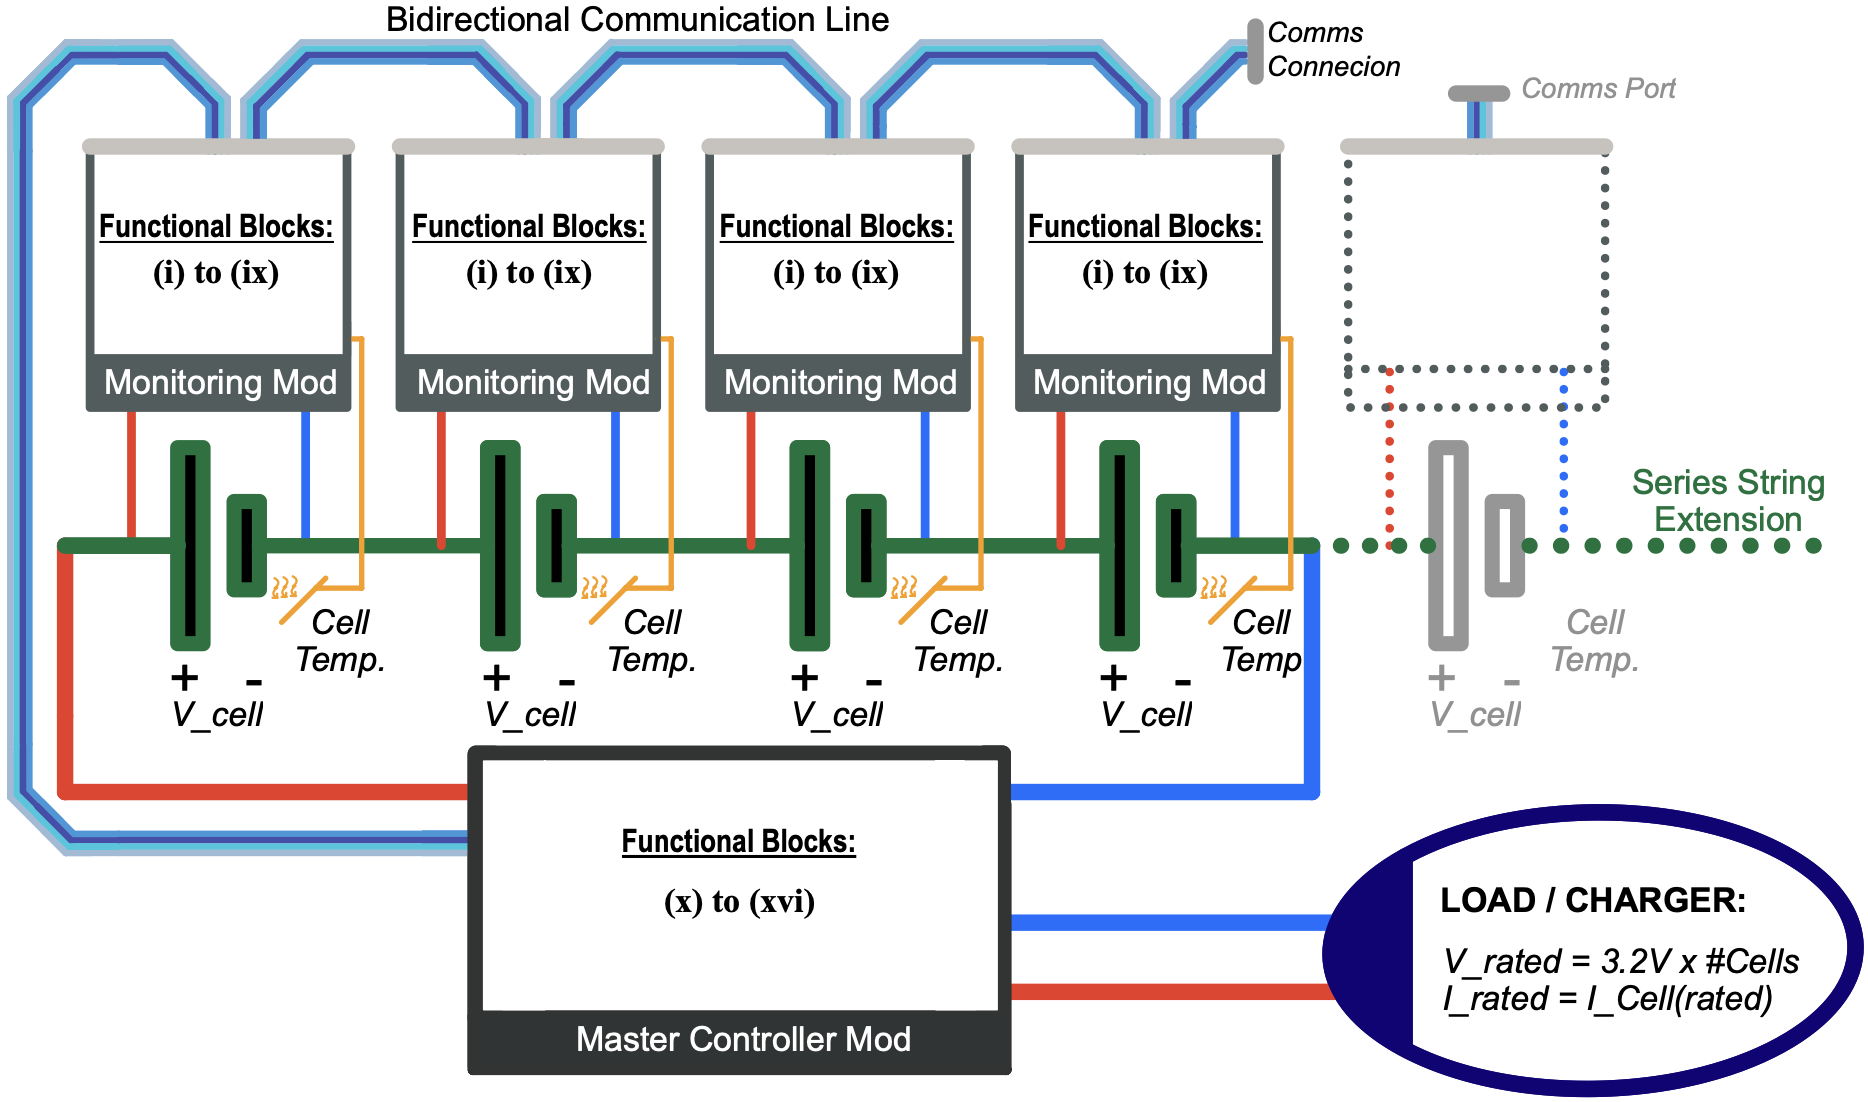
\includegraphics[width=0.7153\textwidth]{Skripsie_LaTeXTemplate/Figures/system_BLOCK_dia.png}
\caption{System Design Functional Blocks}
\label{fig:systOVV_Diagram}
\end{figure}
\noindent
The design of the BMS is organized into distinct functional blocks, each associated with specific subsystems. For a detailed breakdown of these blocks as depicted in figure \ref{fig:systOVV_Diagram}, refer to the subsequent table outlining the primary components of the design.
\begin{table}[h]
    \centering
    \caption{Functional Blocks and Subsystems}
    \label{tab:functional_subsystems}
    \begin{tabular}{|p{0.6cm}|p{6.cm}|p{8.4cm}|}
        \hline
        \textcolor{white}{.} & \textbf{Functional Block} & \textbf{Subsystems} \\
        \hline
        \hline
        \textcolor{white}{.} & \ref{subsec:moni_mods} \emph{Monitoring Module:} & \textcolor{white}{.} \\
        \hline
        \textbf{i} & \hyperref[subsubsec:MM_terminals_dsgn]{Cell Connection} & Parasite hookup \& Inline fuse protection \\
        \hline
        \textbf{ii} & \hyperref[subsubsec:PWR_supply_dsgn]{Voltage Regulation} & 5V Boost power supply \\
        \hline
        \textbf{iii} & \hyperref[subsubsec:force_RESET]{Supply Jumper \& Force Reset} & Programmmer mode \& Mosfet hard reset \\
        \hline
        \textbf{iv} & \hyperref[subsubsec:MM_MC]{Monitoring Microcontroller} & DFR(ATmega32U4) Arduino-Based System \\
        \hline
        \textbf{v} & \hyperref[subsubsec:IntTemp_and_DB_LED]{Onboard Diagnostics} & Internal temperture sensor \& Debug LEDs \\
        \hline
        \textbf{vi} & \hyperref[subsubsec:adc_design]{Cell Voltage Measurement} & Analog to digital converter \& precision reference \\
        \hline
        \textbf{vii} & \hyperref[subsubsec:DL_Designn]{Cell Balancing} & Mosfet passive dump load  \\
        \hline
        \textbf{viii} & \hyperref[subsubsec:ExtTemp_]{Cell Temperature Measurement} & External sensor for ambient temperature \\
        \hline
        \textbf{ix} & \hyperref[subsubsec:iso_COMS]{Isolated Module Communication} & UART isolation \& transceiver logic \\
        \hline
        \textcolor{white}{.} & \ref{subsec:mstr_contt} \emph{Master Controller:} & \textcolor{white}{.} \\
        \hline
        \textbf{x} & \hyperref[subsubsec:mstr_terminals_dsgn]{Terminals \& Fuse Protection} & Battery \& load/charger connection \\
        \hline
        \textbf{xi} & \hyperref[subsubsec:mstr_Supp]{Power Supply} & 5V Buck converter \\
        \hline
        \textbf{xii} & \hyperref[subsubsec:ESP32_dsgn]{Master Microcontroller} & ESP32 DevKitcV4 Arduino-Based System\\
        \hline
        \textbf{xiii} & \hyperref[subsubsec:cur_sen_design]{Battery Current Measurement} & Series connected sensor \\
        \hline
        \textbf{xiv} & \hyperref[subsubsec:LCD_Dsgn]{System Information Display} & LCD and I2C interface \\
        \hline
        \textbf{xv} & \hyperref[subsubsec:relay_Dsgn]{Load/Charge Disconnect} & Latching DC contactor \\
        \hline
        \textbf{xvi} & \hyperref[subsubsec:iso_COMS_Mstr]{Scalable Isolated Communication} & Broadcast UART isolation \\
        \hline
    \end{tabular}
\end{table}

\noindent
The development process of each element in Table \ref{tab:functional_subsystems} will be presented in the subsections: \ref{subsec:moni_mods} \& \ref{subsec:mstr_contt}. a Holistic and comprehensive design process was adopted, where the PCB design, circuit element design, and design calculations were performed simultaneously. This approach ensured a seamless integration between the circuitry and the PCB layout, resulting in an optimized hardware design. Each step of the design process involved meticulous attention to detail, considering factors such as component specifications, performance requirements, and manufacturability. Component selection played a pivotal role in achieving the desired functionality and reliability of the system. Extensive research was conducted, sifting through a vast array of datasheets to identify the most suitable components for each specific application.
%########################################################
\section{Monitoring Modules Design}\label{subsec:moni_mods}
%########################################################
\subsubsection{Design Outline}\label{subsec:mmmm1}
%########################################################
\begin{figure}[h!]
\centering
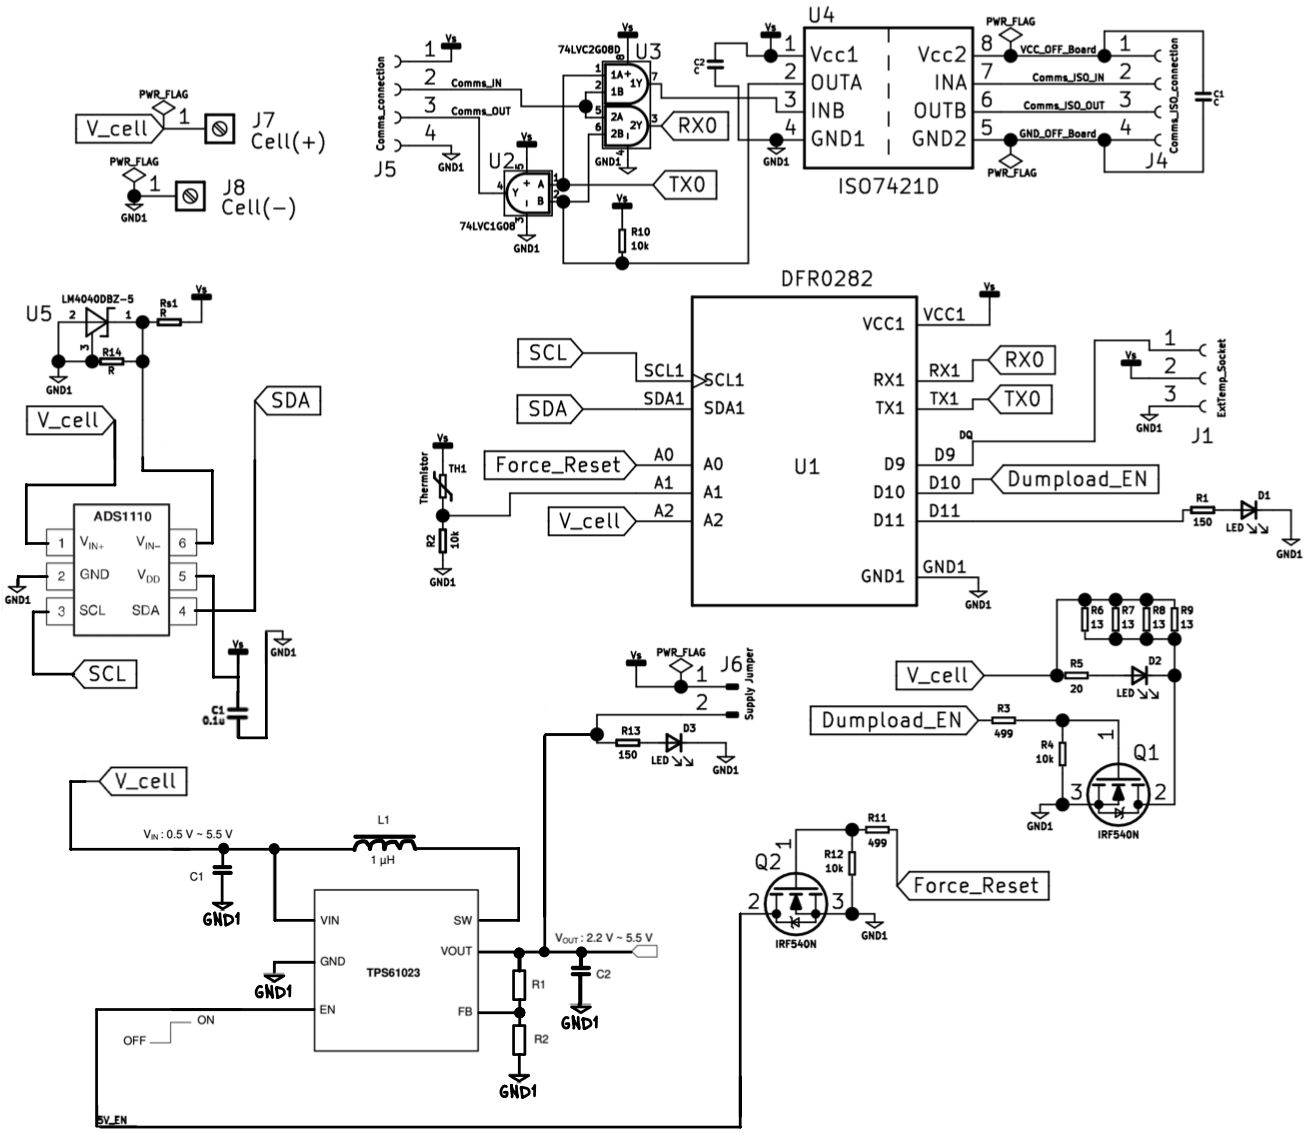
\includegraphics[width=0.9\textwidth]{Skripsie_LaTeXTemplate/Figures/Monitor_Schematic.png}
\caption{Monitoring Module Schematic Diagram}
\label{fig:Monitor_Schema}
\end{figure}

\noindent
Refer to Figure \ref{fig:Monitor_Schema} above for the comprehensive schematic of the monitoring system modules. As delineated in the system overview, the design comprises distinct subsystems working in tandem to form a precise measurement and control platform. A thorough examination of each subsystem's circuit design and component selection is presented in the subsequent section. The \hyperref[subsec:mmmm3]{PCB design} further demonstrates the system's adherence to the design requirements to fit on top of a prismatic LFP cell.
%########################################################
\subsubsection{Circuit Designs \& Component Selection}\label{subsec:mmmm2}
%########################################################
\textbf{\emph{Cell Connection}}\label{subsubsec:MM_terminals_dsgn}

\begin{figure}[h!]
\centering
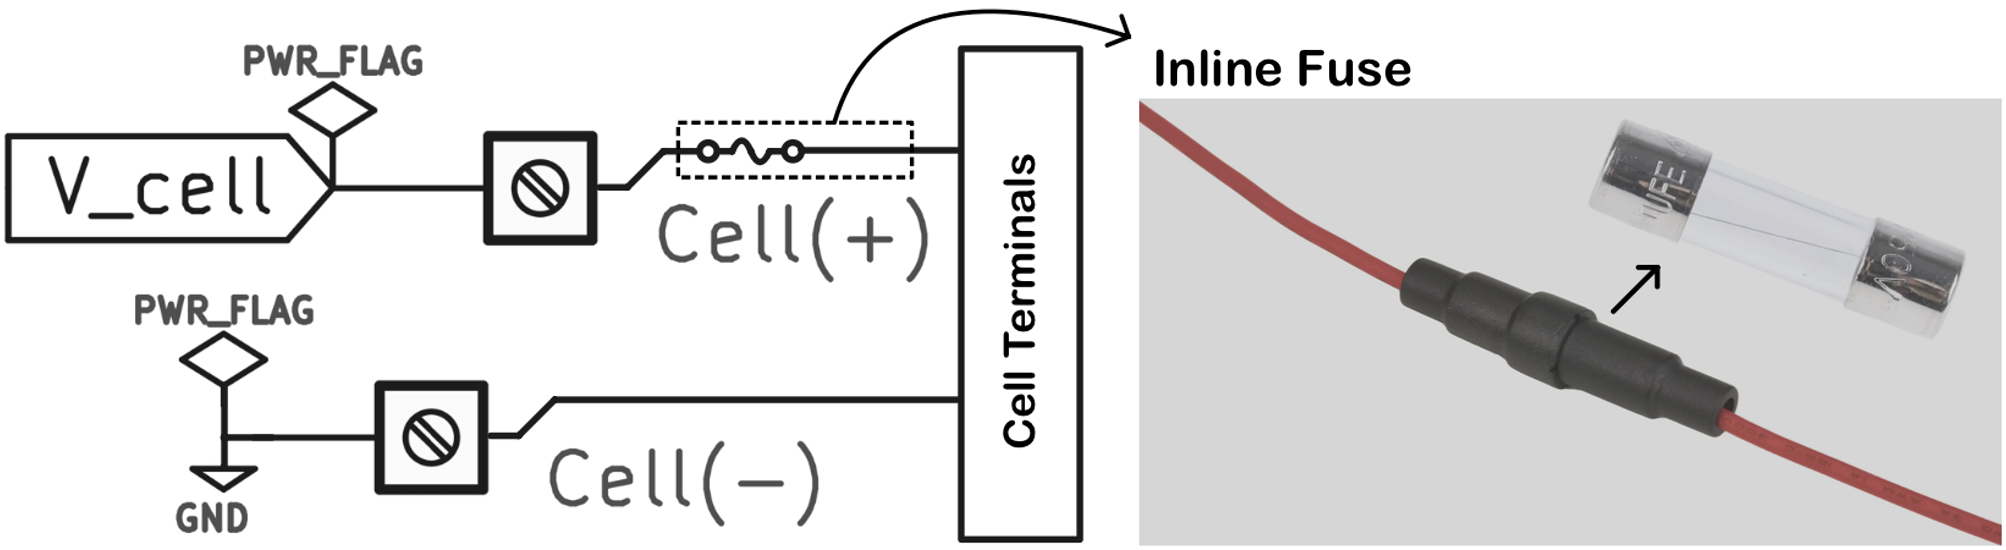
\includegraphics[width=0.4\textwidth]{Skripsie_LaTeXTemplate/Figures/MM_Terminals_Designn.png}
\caption{Monitoring Mod Terminals and Fuse Protection \cite{inlineFuse}}
\label{fig:MM_D9}
\end{figure}
\noindent
A two-pin through-hole PCB connector facilitates cell connection, employing a METZ Connect terminal block rated at 15A to ensure reliable connection beyond peak current demands. The monitoring boards, connecting in parallel to each cell within a series, enable module data acquisition and power draw from the data line, negating external power supply needs. Over-current protection is implemented with a 5mm x 20mm glass fuse, rated at 1.5A, linking the cell's positive terminal to the module, allowing safe 1A discharge by the balancing load during monitoring. While resettable fuses could improve future designs, they are not essential for the current prototype.\newline\newline
%########################################################
\noindent
\textbf{\emph{Voltage Regulation}}\label{subsubsec:PWR_supply_dsgn}\newline
\noindent
To ensure the high precision monitoring system functions optimally, it is crucial to guarantee a stable and accurate power supply to the board. While the system’s microcontroller can operate with voltage as low as 3V, it can’t reach its full functionality. Hence, the voltage level of the 3.2V LFP cell is insufficient to power the board correctly. The voltage is also fluctuating when the cell is being discharged and the ADC used to measure the cell voltage needs a high precision fixed reference voltage to obtain accurate measurements. For a solution we require a voltage step up to 5V, this will also provide a higher logic level for better resolution in the measurements.  

\begin{figure}[h!]
\centering
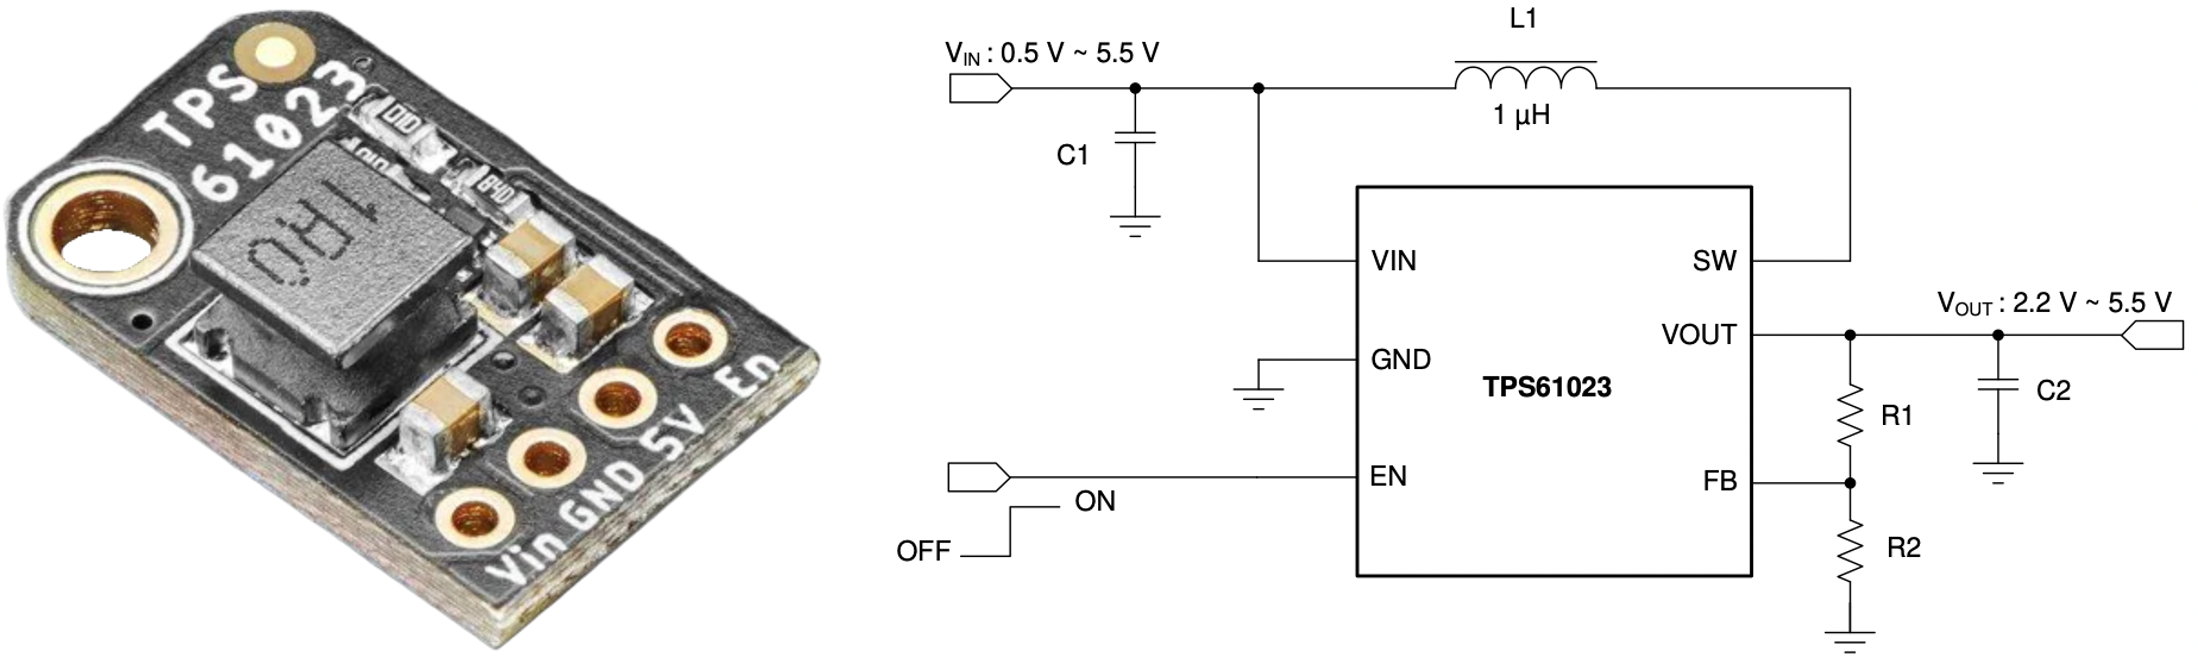
\includegraphics[width=0.6\textwidth]{Skripsie_LaTeXTemplate/Figures/PwrSupp_Designn.png}
\caption{MiniBoost 5V \cite{5vSupply}}
\label{fig:MM_D8}
\end{figure}
\noindent
a Mini-booster utilizing a charge-pump topology with the TPS61023 chip from Texas Instruments is used to preform the voltage regulation. The booster can supply up to 1A current at 5V with a 1\% precision making it the optimal design chose for this purpose.\newline\newline
%########################################################
\noindent
\textbf{\emph{Supply Jumper \& Force Reset}}\label{subsubsec:force_RESET}\newline
\noindent
A power supply jumper is integrated in the battery cell-based system to safely disconnect it from the power source during microcontroller programming, as depicted in figure \ref{fig:MM_D7}. This jumper serves a dual purpose: it establishes a "programmer mode" for safe microcontroller programming and enables reconnection to the power source post-programming, ensuring operational flexibility and system protection during firmware updates.

\begin{figure}[h!]
\centering
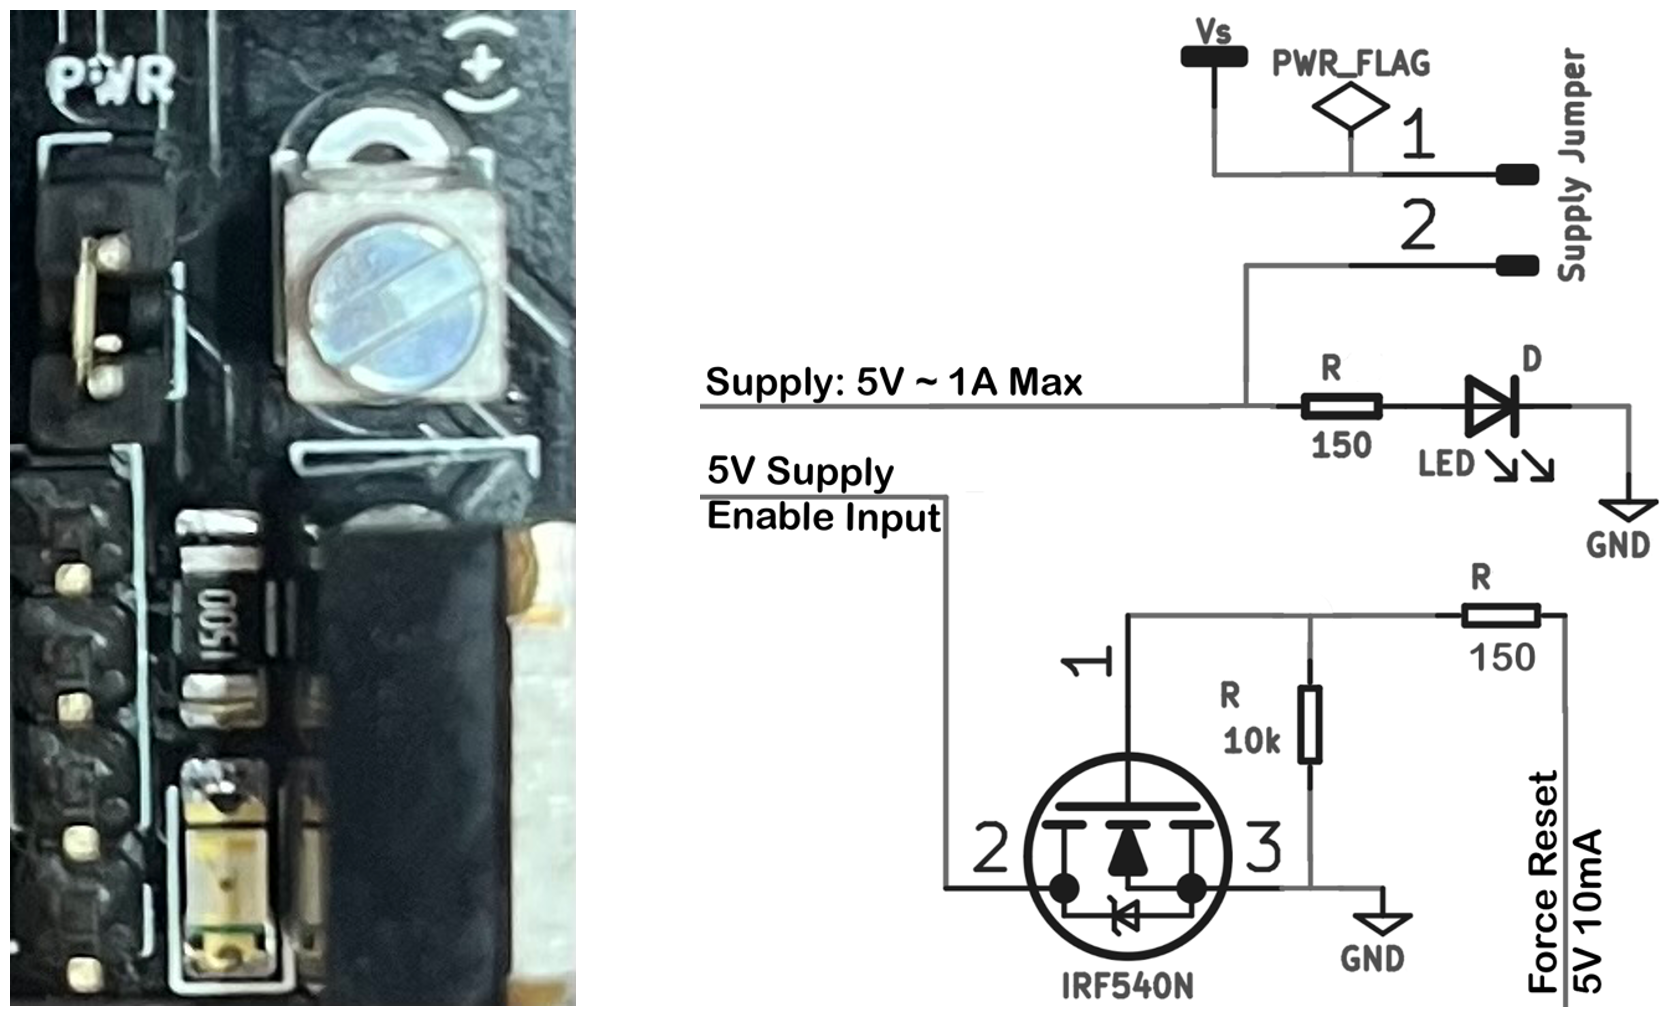
\includegraphics[width=0.38\textwidth]{Skripsie_LaTeXTemplate/Figures/ProgJmp_FReset_Designn.png}
\caption{Power Supply Connection \& Force Reset}
\label{fig:MM_D7}
\end{figure}

\noindent
An emergency reset circuit is included, utilizing a mosfet as a low-side switch to momentarily ground the enable pin of the TPS61023 chip, thereby initiating a system restart. This force reset functionality is vital for addressing unforeseen microcontroller errors, glitches, or transient faults, enabling a quick system return to a known, stable state without manual intervention.\newline\newline
%########################################################
\noindent
\textbf{\emph{Monitoring Microcontroller}}\label{subsubsec:MM_MC}\newline
\noindent
The DFR0282 microcontroller, chosen for its compact size fitting aptly between cell terminals, facilitates on-the-fly programming alterations via its micro-USB feature. Its compatibility with Arduino Leonardo simplifies rapid code modifications in the Arduino environment, meeting the project's technical requisites efficiently.

\begin{figure}[h!]
\centering
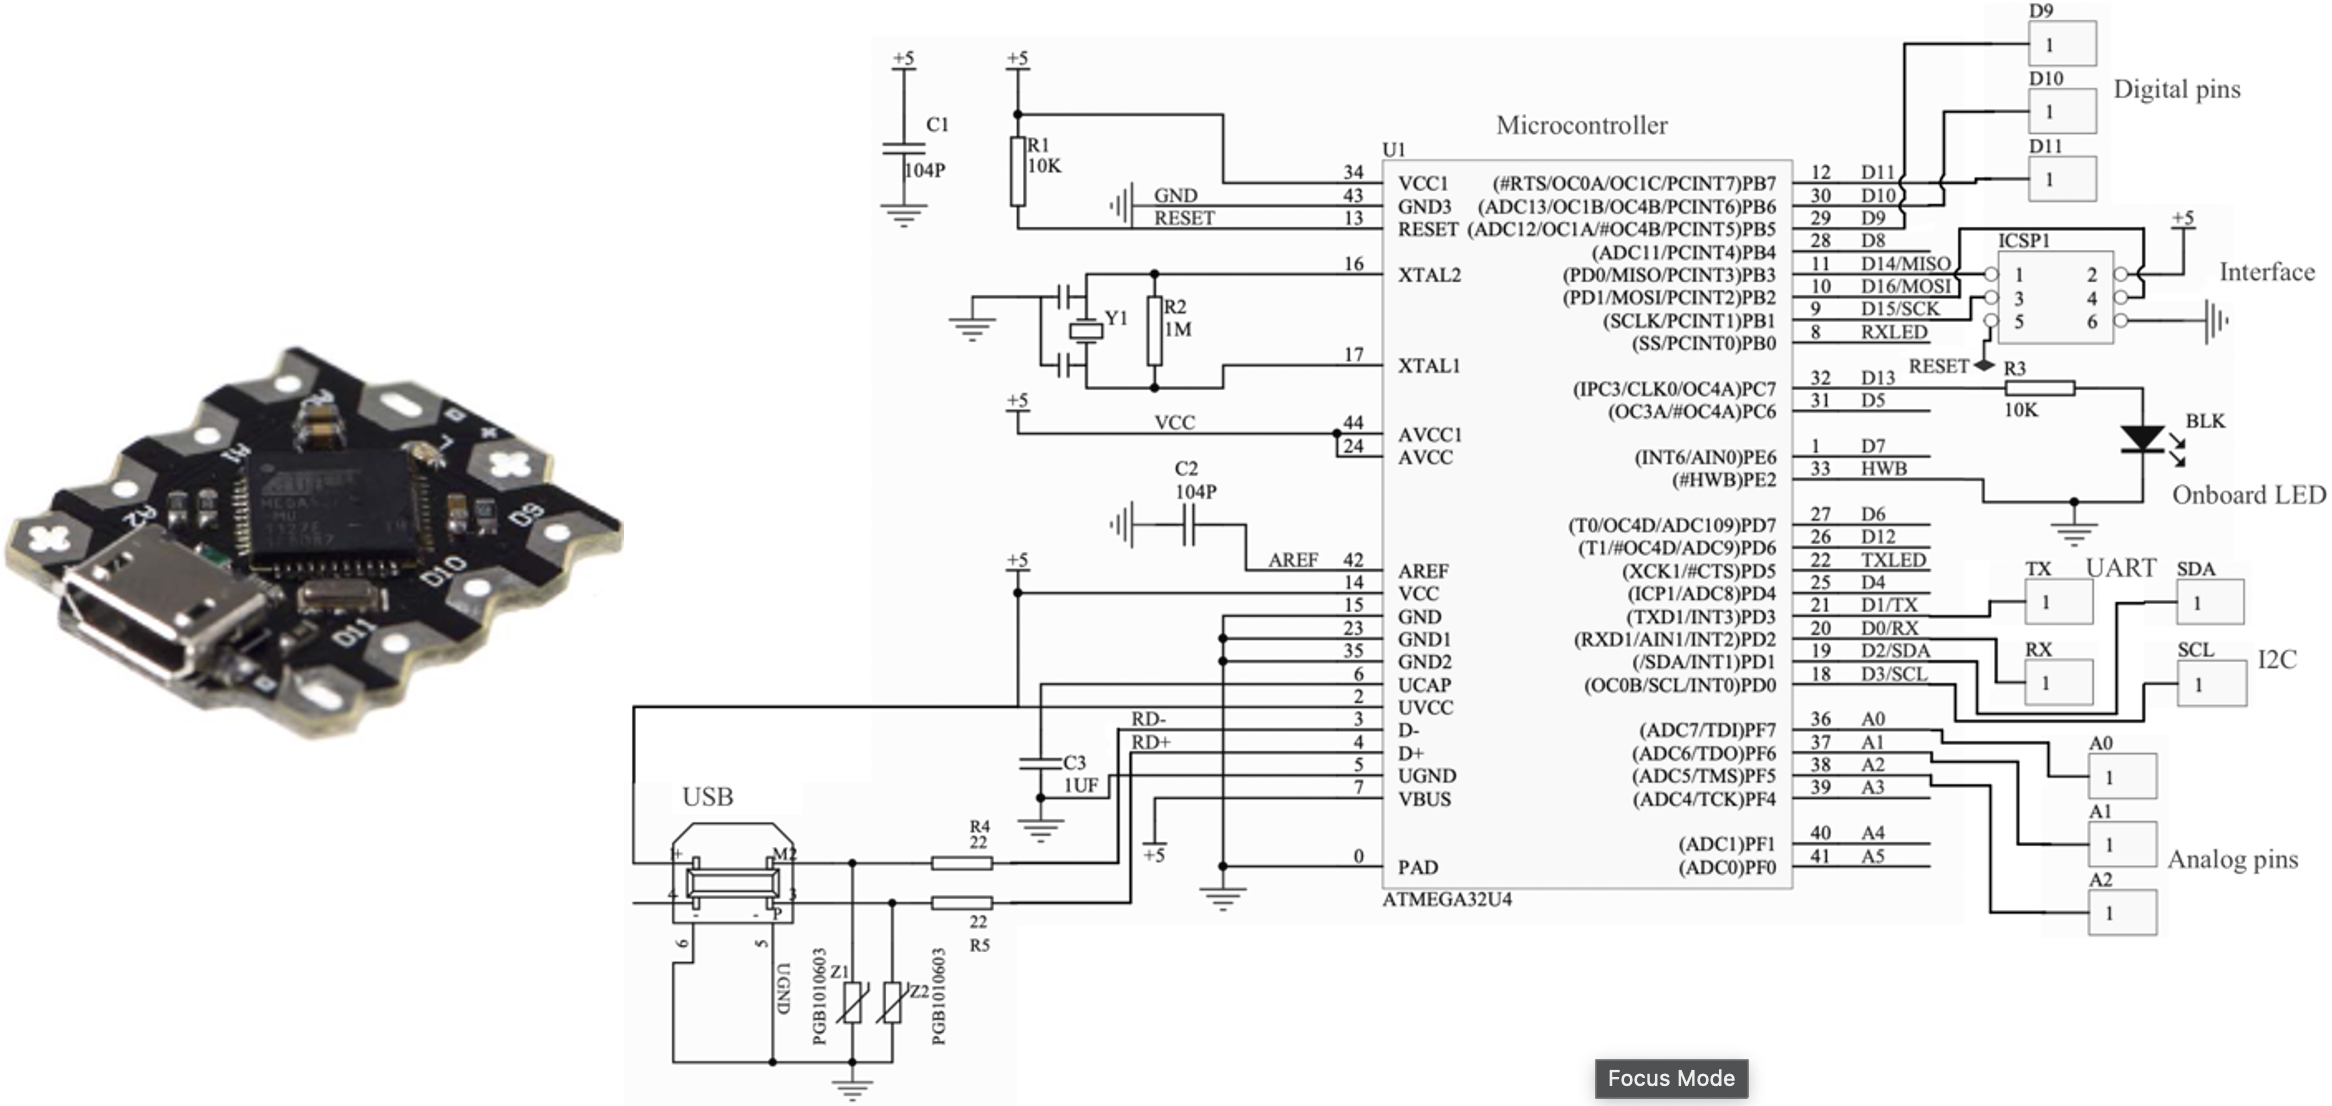
\includegraphics[width=0.7\textwidth]{Skripsie_LaTeXTemplate/Figures/MM_MircoCont_Designn.png}
\caption{DFR0282 - (ATmega32U4) Microcontroller \cite{beetle}}
\label{fig:MM_D6}
\end{figure}

\noindent
Equipped with the ATmega32U4 chip and accompanying conditioning circuitry, the DFR0282 module provides six General Purpose Input/Output (GPIO) pins, I2C, and UART pins. This pin configuration aligns with system requirements, ensuring full utilization of available pins for designated functions as detailed in the subsequent table, thereby enhancing the system's functional efficacy.

\begin{table}[h]
    \centering
    \caption{Monitoring Microcontroller Pin Out}
    \label{tab:Beetle_PinOut}
    \begin{tabular}{|c|c|c|}
        \hline
        \textbf{DFR0282-Pin} & \textbf{Configuration} & \textbf{Utility} \\
        \hline
        \hline
        0 & RX & Serial communication receive channel \\
        \hline
        1 & TX & Serial communication transmit channel \\
        \hline
        2 & SDA & I2C data channel for external ADC \\
        \hline
        3 & SCL & Clock channel for I2C sampling \\
        \hline
        9 & Digital GPIO & External temperature sensor digital input \\
        \hline
        10 & Digital GPIO & Cell balancing dump-load enable pin \\
        \hline
        11 & PWM Channel & LED for system debug messages \\
        \hline
        A0 & Digital GPIO & Force reset enable pin \\
        \hline
        A1 & Analog Channel & Internal temperature sensor analog input \\
        \hline
        A2 & Analog Channel & Cell voltage analog input \\
        \hline
    \end{tabular}
\end{table}

%########################################################
\noindent
\textbf{\emph{Onboard Diagnostics}}\label{subsubsec:IntTemp_and_DB_LED}

\begin{figure}[h!]
\centering
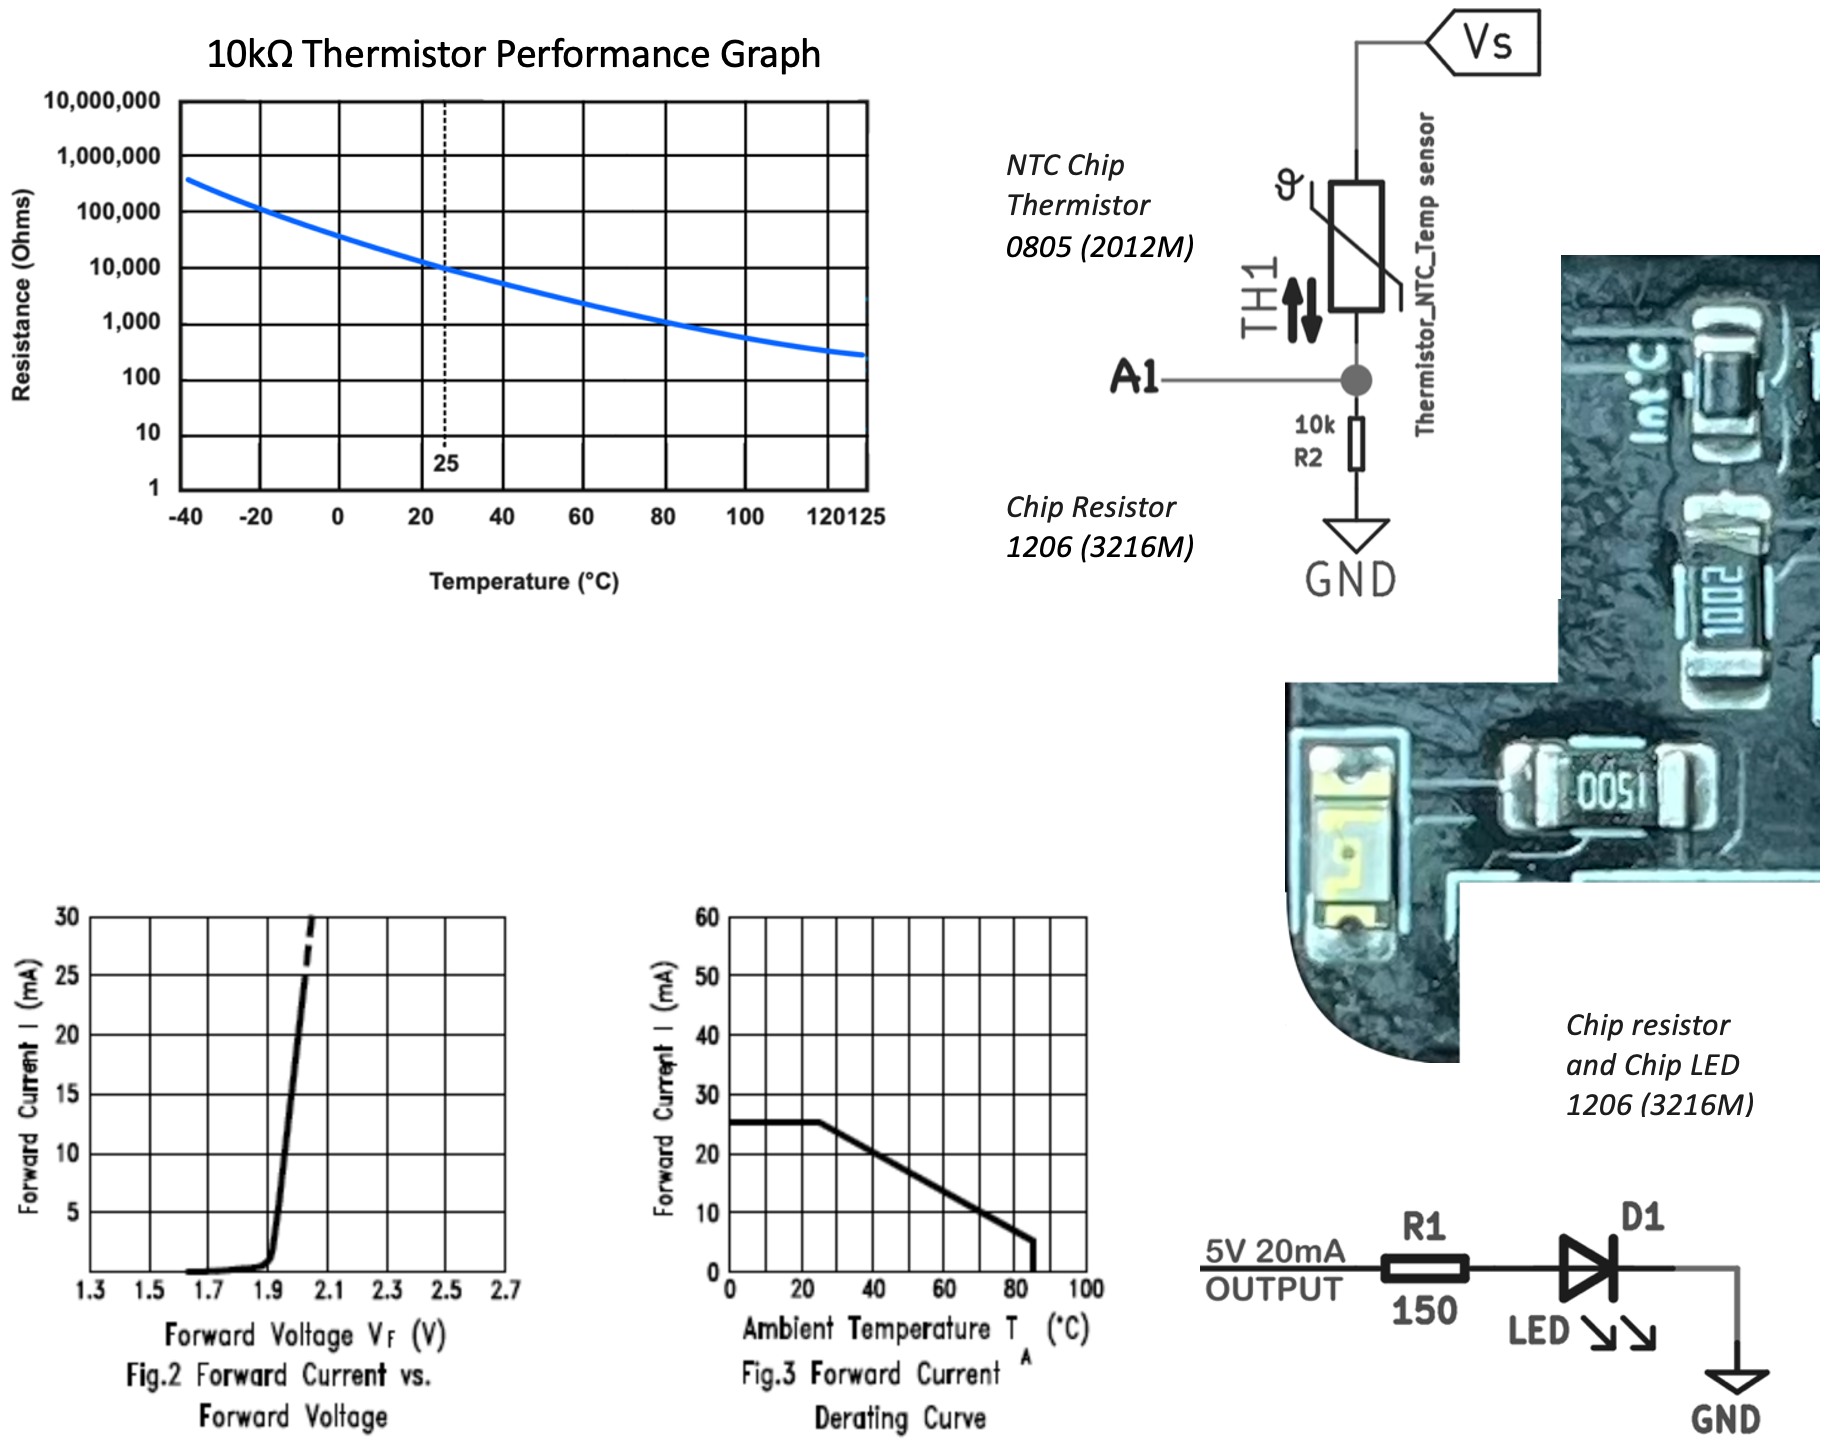
\includegraphics[width=0.5\textwidth]{Skripsie_LaTeXTemplate/Figures/IntTemp_LED_Designn.png}
\caption{NTC Temperature Sensor \cite{IntTemp} \& Debug LED \cite{LED}}
\label{fig:MM_D5}
\end{figure}
\noindent
\emph{Internal Temperature Measurement:}\newline
\noindent
An on-board temperature sensor is crucial for real-time thermal management, ensuring operational safety and optimizing performance. The circuit employs a TE Connectivity Thermistor in a voltage divider configuration with a fixed \(10k\Omega\) resistor. The thermistor's resistance (\( R_{th} \)) varies with temperature (graph presented in figure \ref{fig:MM_D5}), affecting the voltage (\( V_{out} \)) at the microcontroller's analogue input pin as per the following equations.
\[ R_{th} = R_0 \cdot \exp \left( \frac{\beta}{T} - \frac{\beta}{T_0} \right) \hspace{0.5cm} \& \hspace{0.5cm} V_{out} = 5V \cdot \left( \frac{R_{th}}{R + R_{th}} \right) \]
\noindent
\emph{System Debug LED:}\newline
\noindent
An LED indicator is instrumental for providing immediate, visible feedback regarding system debug messages, aiding in swift diagnosis and rectification of operational issues.
\[ R_{limiting} = \frac{V_s - V_f}{I} = \frac{5V - 2V}{0.02A} = 150 \Omega \]
%########################################################
\noindent
\textbf{\emph{Cell Voltage Measurement}}\label{subsubsec:adc_design}

\begin{figure}[h!]
\centering
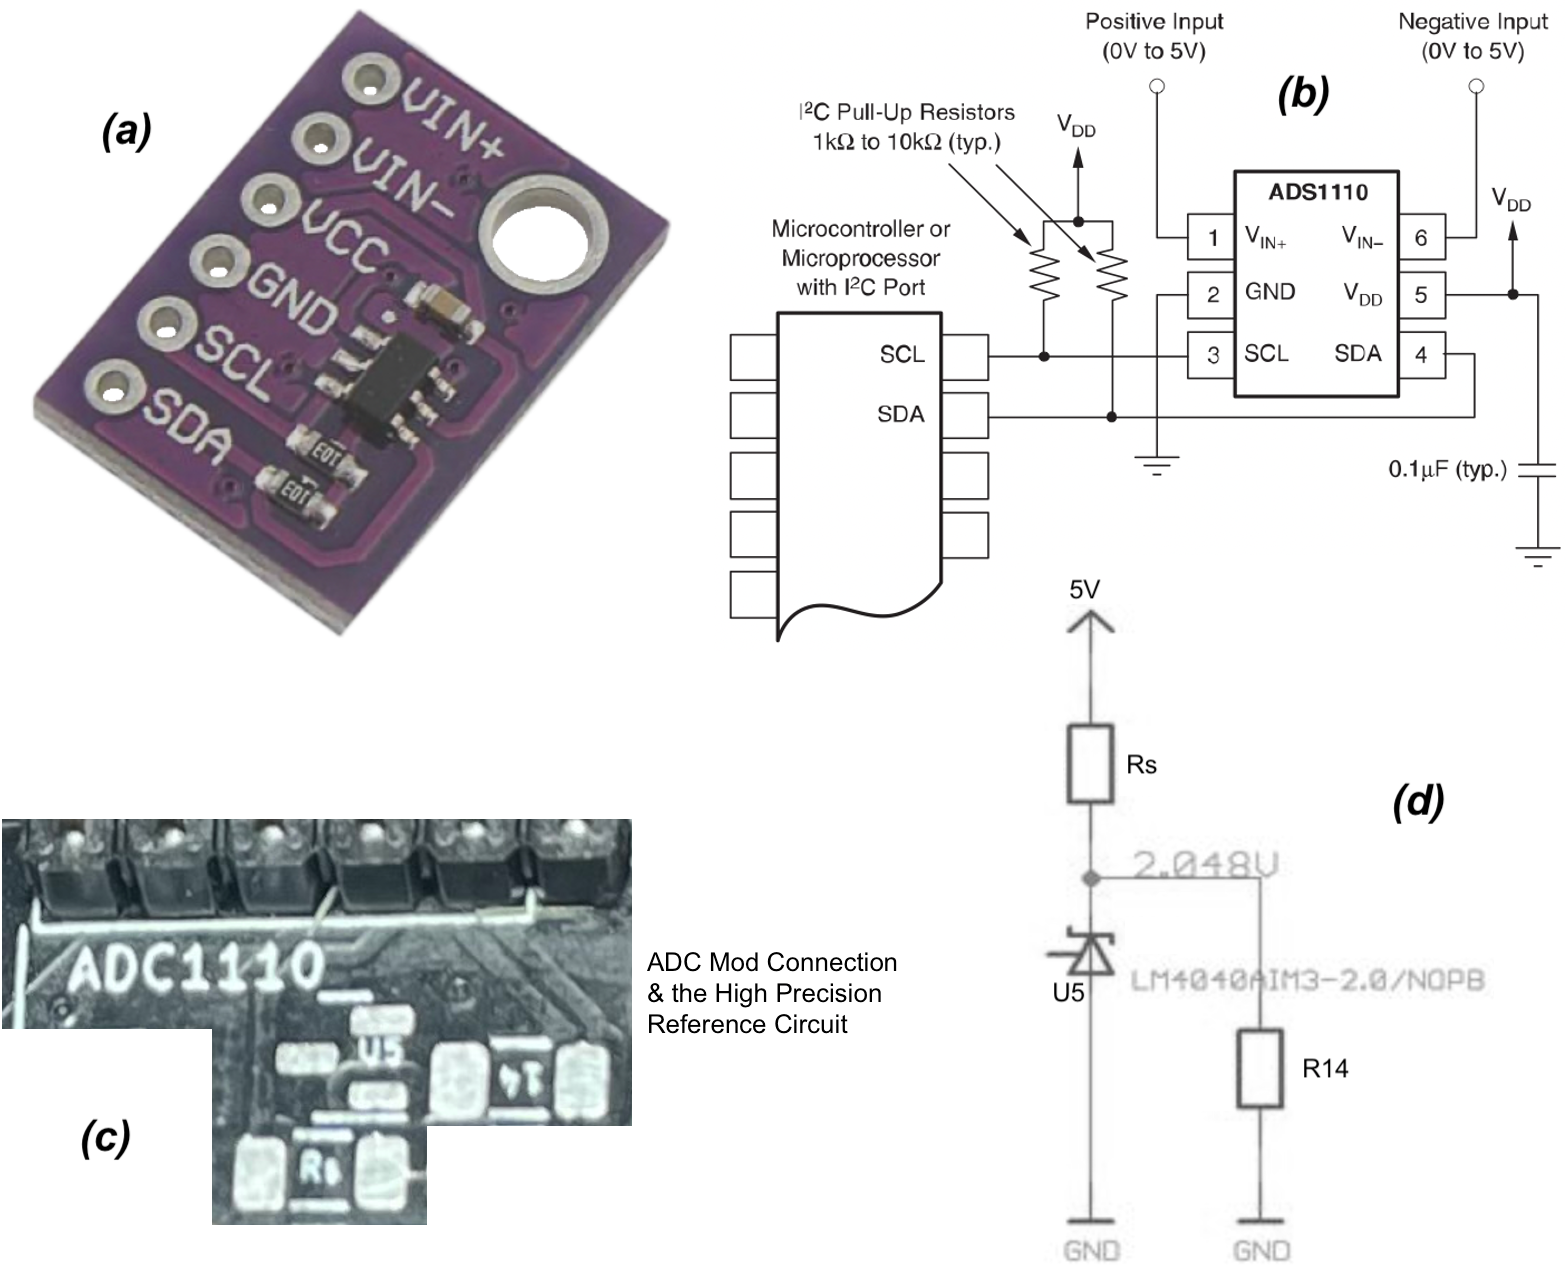
\includegraphics[width=0.5\textwidth]{Skripsie_LaTeXTemplate/Figures/ADC_Designn.png}
\caption{(a)16bit ADC (b)ADS1110 Design\cite{TheADC} (c)2.048V Ref. (d)LM4040 Design\cite{PrecRef}}
\label{fig:MM_D1}
\end{figure}
\noindent
Accurate cell voltage measurement is crucial for cell monitoring. While the DFR0282 microcontroller has an onboard 8-bit ADC for backup measurement, a high-precision measurement is achieved using an external 16-bit ADC, the ADS1110. As depicted in figure \ref{fig:MM_D1}\textbf{(a)}, the ADS1110 interfaces with the microcontroller via 2K2 pull-up resistors on its I2C lines, operating at a baud rate of 9600. Powered by the microcontroller's 5V and ground lines, the ADS1110, with a sample rate of 240 SPS, offers a resolution of approximately 0.00003125V, as calculated by the formula below.
\[
\text{Resolution} = \frac{V_{\text{ref}}}{2^{\text{N}}} = \frac{2.048V}{2^{\text{16 bits}}} = 31.25 \mu
\]
\noindent
A stable external 2.048V reference is essential for maintaining the ADC's precision, as depicted in figure \ref{fig:MM_D1}\textbf{(c)}. The circuit, as shown in figure \ref{fig:MM_D1}\textbf{(d)}, utilizes the LM4040AIM3-2.0/NOPB shunt voltage reference chip, a \(750 \, \Omega\) series resistor (\(R_s\)), and a \(10 \, k\Omega\) shunt resistor (\(R_{sh}\)). The anode and NC pin of the LM4040AIM3-2.0/NOPB are grounded, while the cathode pin connects to a junction, also connected to \(R_s\) and \(R_{sh}\).
\[
I_{ref} = \frac{V_{supply} - V_{ref}}{R_s} = \frac{5V - 2.048V}{750 \, \Omega}
\]
\noindent
The formula above determines the current through the LM4040AIM3-2.0/NOPB chip (\(I_{ref}\)), and the total current through \(R_s\) is given by the following equation.
\[
I_{R_s} = I_{ref} + I_{sh} = I_{ref} + \frac{V_{ref}}{R_{sh}}
\]
\noindent
This design ensures a stable reference voltage across various operating conditions, thus preserving the accuracy of the 16-bit ADC for precise cell voltage measurement.\newline\newline
%########################################################
\noindent
\textbf{\emph{Cell Balancing}}\label{subsubsec:DL_Designn}\newline
\noindent
Cell balancing is crucial for managing LFP battery packs where series-connected cells exhibit variations in capacity, internal resistance, and charge characteristics, leading to voltage imbalances that affect battery life and safety. It aims to equalize the SOC across cells. Two prevalent techniques exist: active and passive balancing. Active balancing employs switches and capacitors for charge transfer, presenting efficiency albeit at higher complexity and cost. Conversely, passive balancing dissipates excess charge through resistors, offering simplicity, cost-effectiveness, and reliability, often making it a preferred choice in robust system designs over the marginal efficiency benefits of active balancing.

\begin{figure}[h!]
\centering
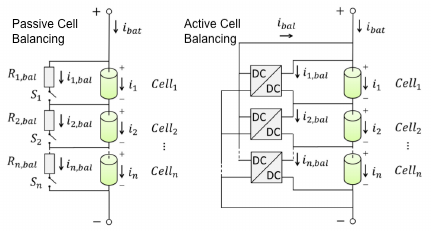
\includegraphics[width=0.4\textwidth]{Skripsie_LaTeXTemplate/Figures/actVSpass.png}
\caption{Activate vs Passive Balancing \cite{generic}}
\label{fig:actVSpass}
\end{figure}
\noindent
A passive balancing circuit was chosen for the cell modules, with balancing current as a pivotal factor. To ascertain the dump load size for each cell in a 105Ah 3.2V LFP series-connected battery pack, it's necessary to consider both the maximum charging current and the required balancing current for effective balancing. The EVE Energy cell datasheet \cite{eve} recommends a maximum charging current of 1C (105A) for the battery pack, thus a balancing current of about 1\% of the maximum charging current, or approximately 1A, is deemed suitable for the dump load design per cell.

\begin{figure}[h!]
\centering
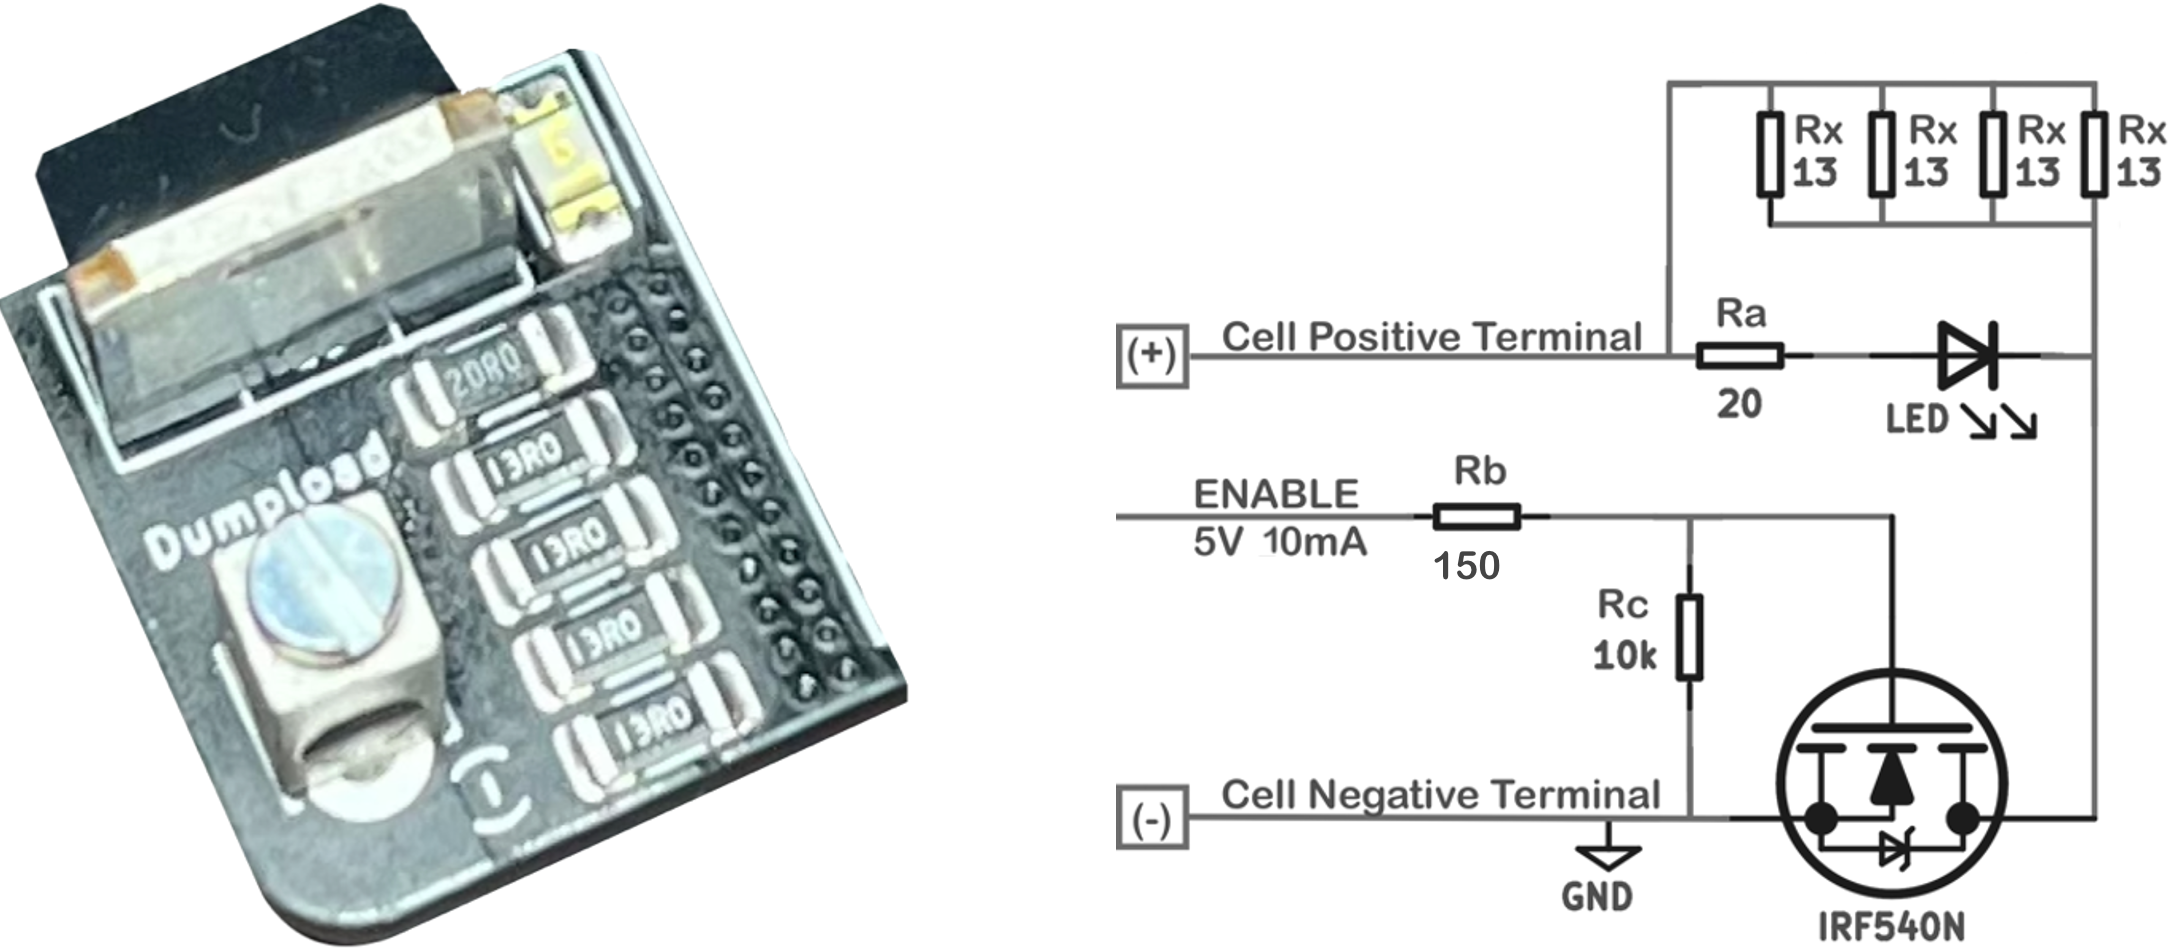
\includegraphics[width=0.5\textwidth]{Skripsie_LaTeXTemplate/Figures/DmpLoad_Designn.png}
\caption{Balancing Dump-load Design}
\label{fig:MM_D3}
\end{figure}
\noindent
The load is made up of four $13\Omega$ chip resistors in parallel.
\begin{equation}
R_{\text{Dump-Load}} = (\frac{1}{13\Omega} \cdot 4)^{-1} = 3.25\Omega
\end{equation}
This resistance value results in a balancing current just below 1A.
\begin{equation}
I_{\text{Balancing}} = \frac{3.2V}{3.25\Omega} = 0.985A
\end{equation}
To ensure that the resistors are thermally capable of handeling the balancing current we need to look at their power rating.
\begin{equation}
P_{\text{Dump-Load}}(Min.) = (0.985A)^{2} \cdot 3.25\Omega = 3.153W
\end{equation}
Since the resistors are connected in parallel the power rating for the dumpload is given by the equation below.
\begin{equation}
P_{\text{Dump-Load}} = P_{13\Omega-Resistor} \cdot 4
\end{equation}
\noindent
Therefor a high power thin film $13\Omega$ chip resistor from SUSUMU \cite{CHIPrr}, with a power rating of $1W$ was chosen for safe operation of the load.\newline\newline
\noindent
\emph{Low-side Switch:}\label{subsubsec:LS_SW}\newline
\noindent
The dump-load is controlled by a microcontroller with a desire output of 20mA on its gpio pins. a High signal of 5V on the pin is used to switch a Power Mosfet. The mosfet is used in a low-side switch configuration and has a gate threshold voltage of 2V. The following calculation was done to select the appropriate gate current limiting resistor \cite{mos}.
\begin{equation}
R = \frac{\Delta V}{I_{Gate}} = \frac{5V - 2V}{20mA} = 150\Omega
\end{equation}
\noindent
A $10k\Omega$ resistor is typically used as a pull-down resistor in a 5V system due to its balance of limiting current, reducing power consumption, and ensuring reliable logic level interpretation.\newline\newline
%########################################################
\noindent
\textbf{\emph{Cell Temperature Measurement}}\label{subsubsec:ExtTemp_}\newline
\noindent
Designed to be positioned at the cell's negative terminal (current entry \& exit point), the external temperature sensor, DS18B20, facilitates effective cell thermal monitoring crucial for detecting temperature alterations under heavy loads or charging, thereby enhancing battery safety and efficiency.

\begin{figure}[h!]
\centering
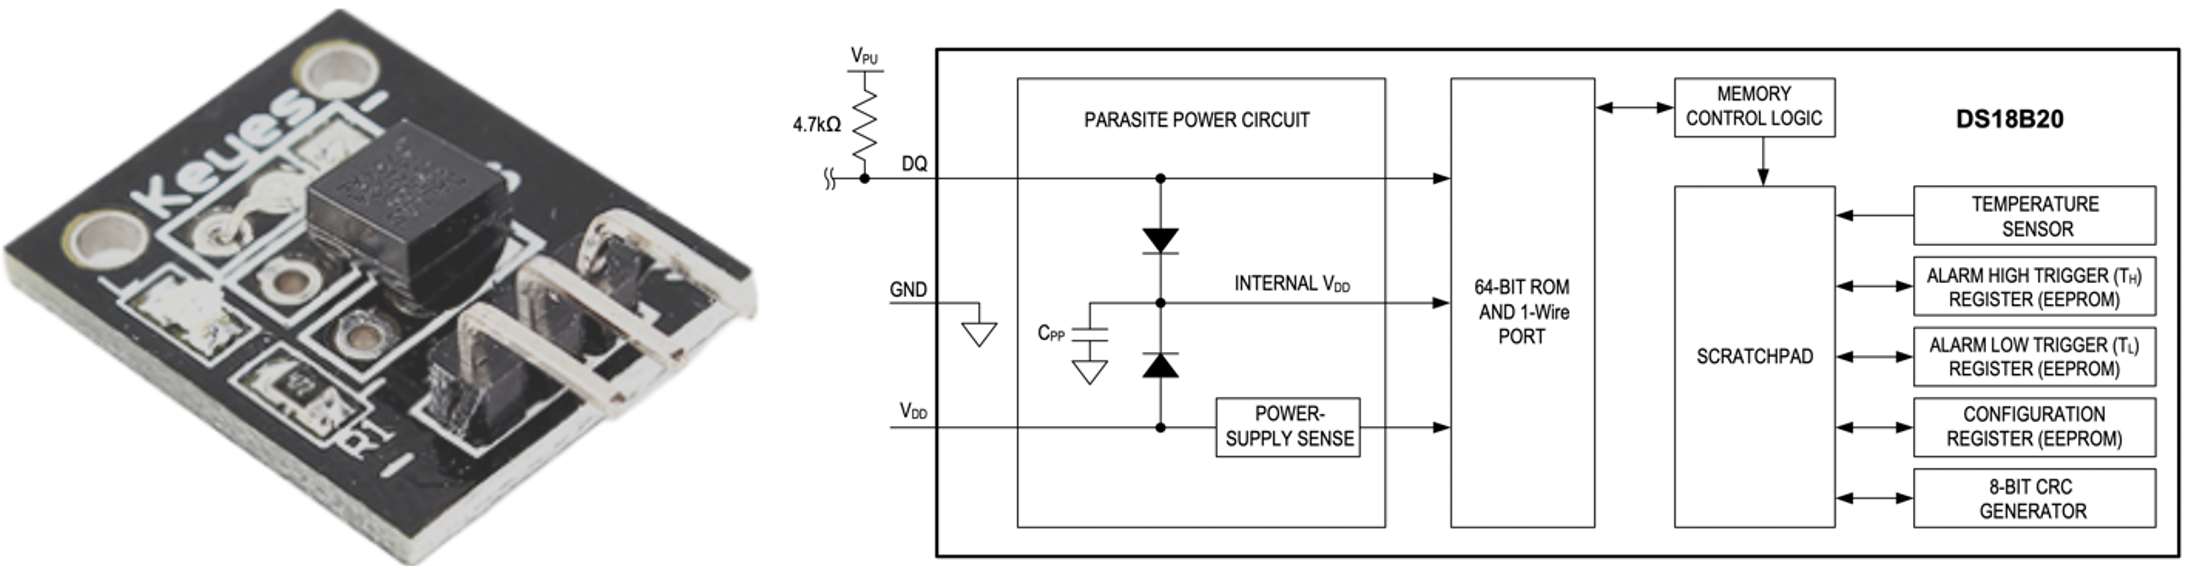
\includegraphics[width=0.65\textwidth]{Skripsie_LaTeXTemplate/Figures/ExtTemp_Designn.png}
\caption{External Temperature Sensor \cite{TheExtTempSen}}
\label{fig:MM_D4}
\end{figure}
\noindent
The DS18B20 ensures ±0.5°C accuracy within a -20°C to +85°C range, extendable to -55°C to +125°C. Operating at 5V with a 9 to 12-bit resolution range and "parasite power" capability, the DS18B20 eliminates the need for external power, making it a proficient choice for ambient cell temperature monitoring.\newline\newline
%########################################################
\noindent
\textbf{\emph{Isolated Module Communication}}\label{subsubsec:iso_COMS}\newline
\noindent
As delineated in the background study's section \ref{sec:commsMeth}, a comprehensive analysis guided the design choice of the ISO7421D (low-power dual-channel digital isolator chip) from Texas Instruments \cite{isooooCHIP} to isolate UART communication lines. Unlike optocouplers that requires external components for operation, the ISO7421D solely requires two bypass capacitors for supply decoupling. The devised architecture diverges from conventional series-connected isolated daisy-chain or parallel-connected isolated bus lines. Instead, ISO7421D chips are serialized, creating a communication line segmented by isolated barriers, each with two channels: one facilitating data transmission down the stack, and the other, upwards.\newline\newline
\noindent
This arrangement creates a bidirectional communication bus, wherein between each isolating barrier, signals are either tapped off using a receiver or tapped into the communication line via a transmitter, adhering to an asynchronous serial system protocol. Consequently, all modules along the communication line attain broadcast channel read and write access throughout the system. This configuration mitigates the limitations of common all-call and daisy-chain setups, which encounter scalability constraints due to the elevated output impedance on serial communication, attributed to parallel-arranged digital isolator chips. Such impedance escalation prompts the integration of output drivers to ensure proficient message transmission across the communication line. The novel communication system is illustrated in figure \ref{fig:MM_D2} below.

\begin{figure}[h!]
\centering
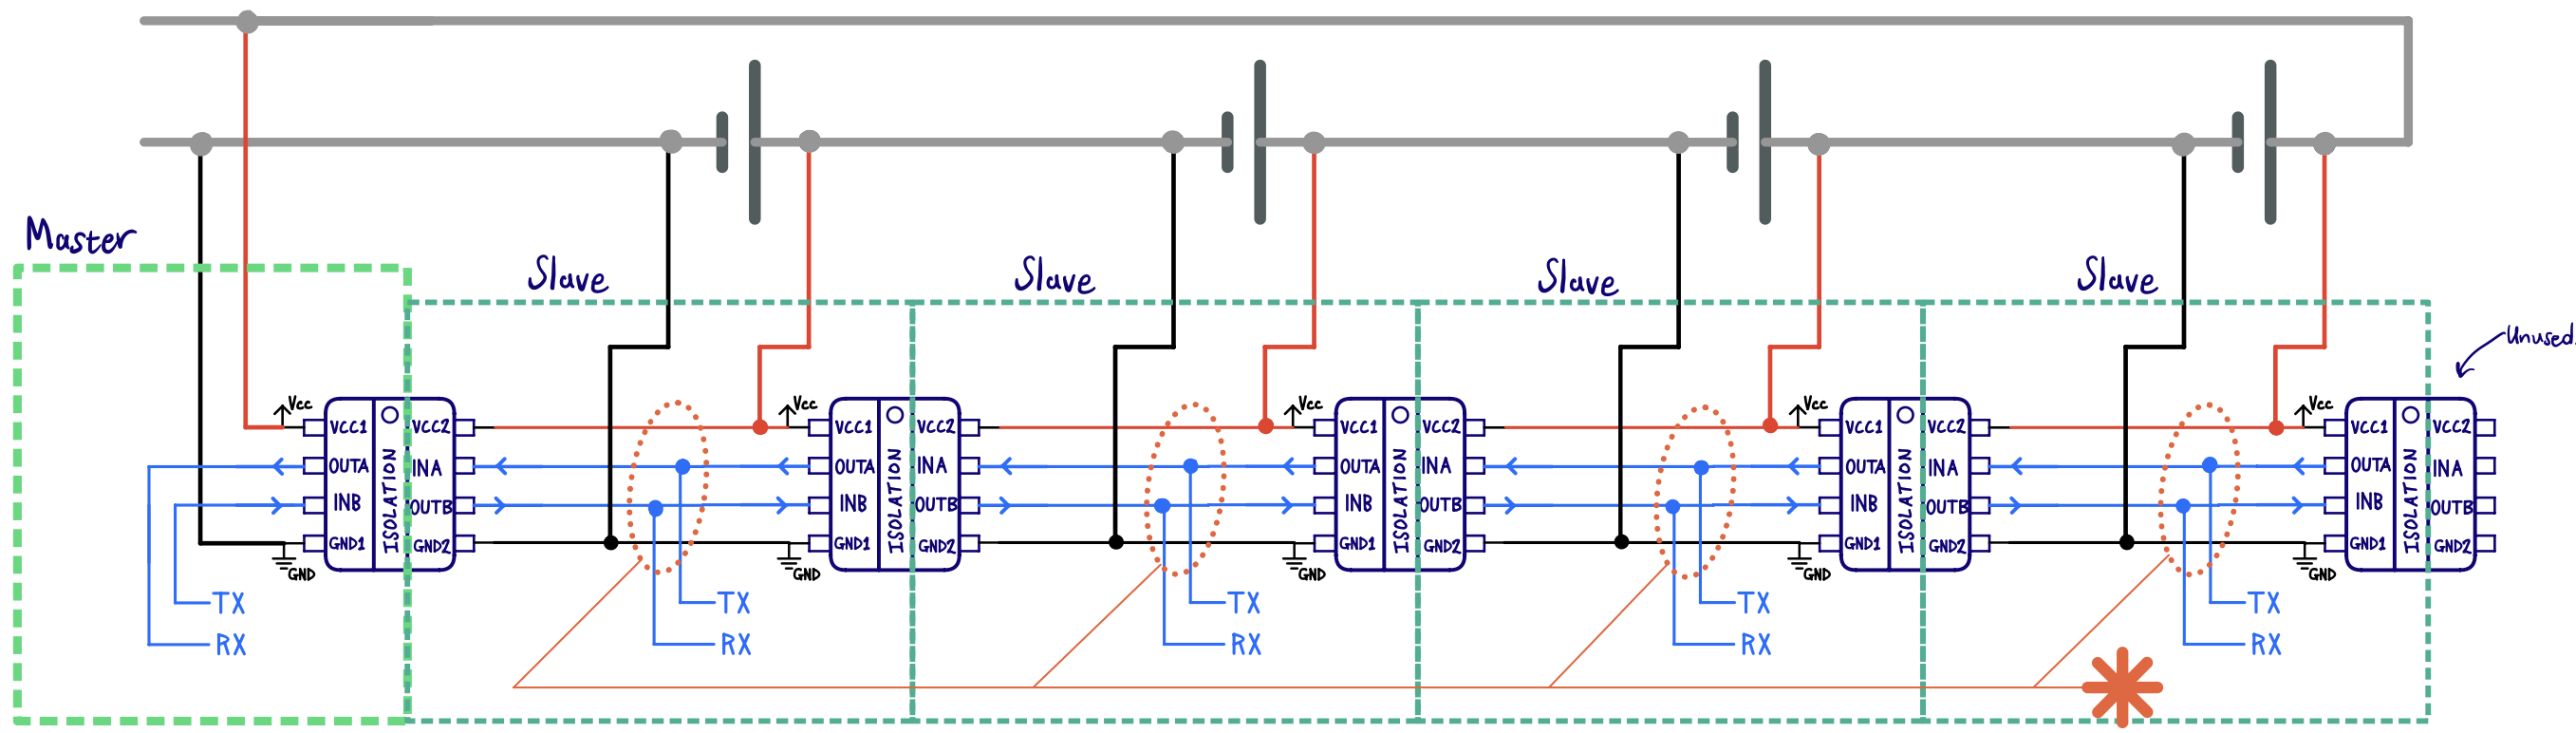
\includegraphics[width=1.0\textwidth]{Skripsie_LaTeXTemplate/Figures/COMMS_SELECT.png}
\caption{Isolated Communication Configuration}
\label{fig:MM_D2}
\end{figure}
\noindent
The design configuration above may incur bus contention (\textcolor{orange}{\textbf{*}}) during simultaneous data transmission by multiple transceivers, resulting in signal interference and data corruption. Addressing this issue involves the utilization of an asynchronous software protocol with sequential program timers, which allocates specific time slots for each transceiver to transmit data, thus eliminating overlap and resolving bus contention. To fortify against unforeseen simultaneous data transmission potentially harmful to the system, a communication bit control logic system, employing SN74LVC2G08 AND-gates from Texas Instruments \cite{isooooCHIP}, was developed, as depicted in figure \ref{fig:buscon} on the next page.\newpage
\begin{figure}[h!]
\centering
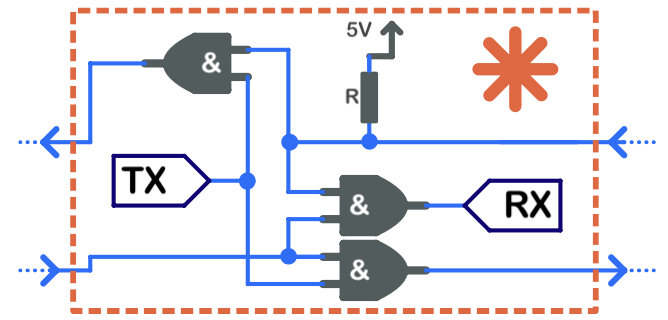
\includegraphics[width=0.28\textwidth]{Skripsie_LaTeXTemplate/Figures/BUS_CON.png}
\caption{Protection Logic Circuit}
\label{fig:buscon}
\end{figure}
\noindent
The final design equipped to each cell monitoring module is presented below in figure \ref{fig:klakom}, highlighted pathways represent the data flow of the communication system.

\begin{figure}[h!]
\centering
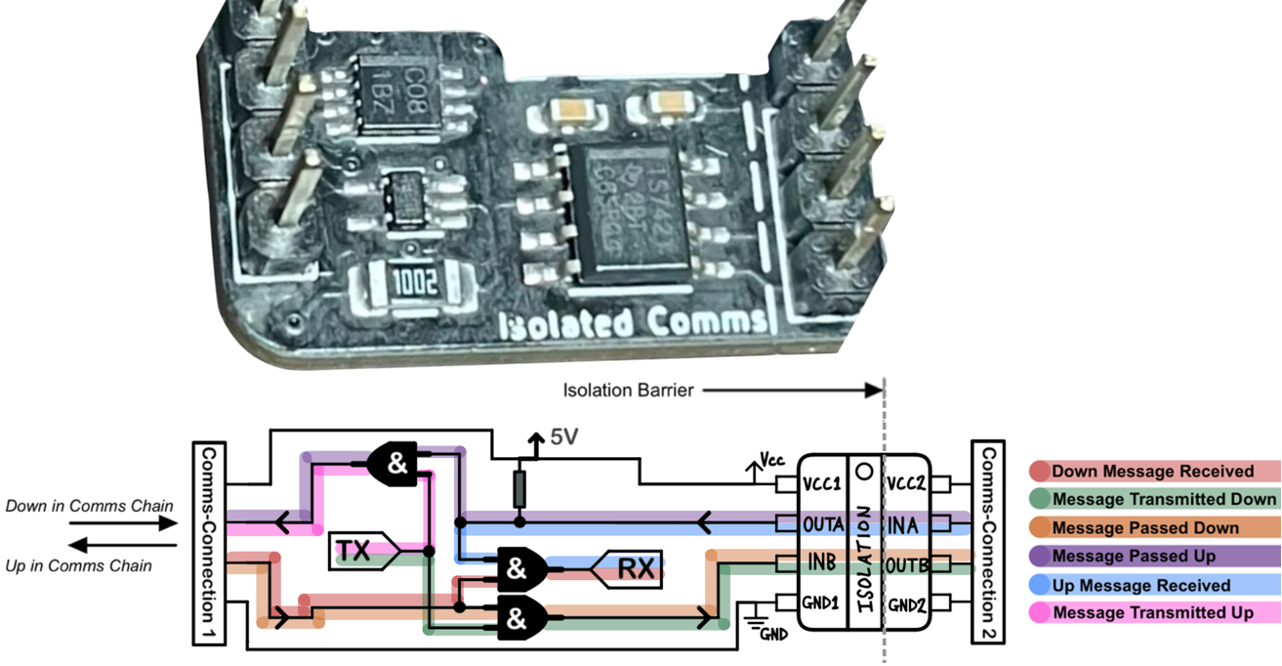
\includegraphics[width=0.75\textwidth]{Skripsie_LaTeXTemplate/Figures/FINAL_KOM.png}
\caption{Isolated Communication System Design}
\label{fig:klakom}
\end{figure}
%########################################################
\subsubsection{Printed Circuit Board Design}\label{subsec:mmmm3}
%########################################################
In the figure below, the left illustrates the PCB design encompassing all copper layers and component footprints selected during the design process of the cell monitoring module. Despite size constraints posing a challenge, the design, as depicted on the right, successfully accommodates a 3D representation of the module between the cell's terminals. Refer to Appendix \ref{appen:cad} for the complete CAD assembly design.

\begin{figure}[h!]
\centering
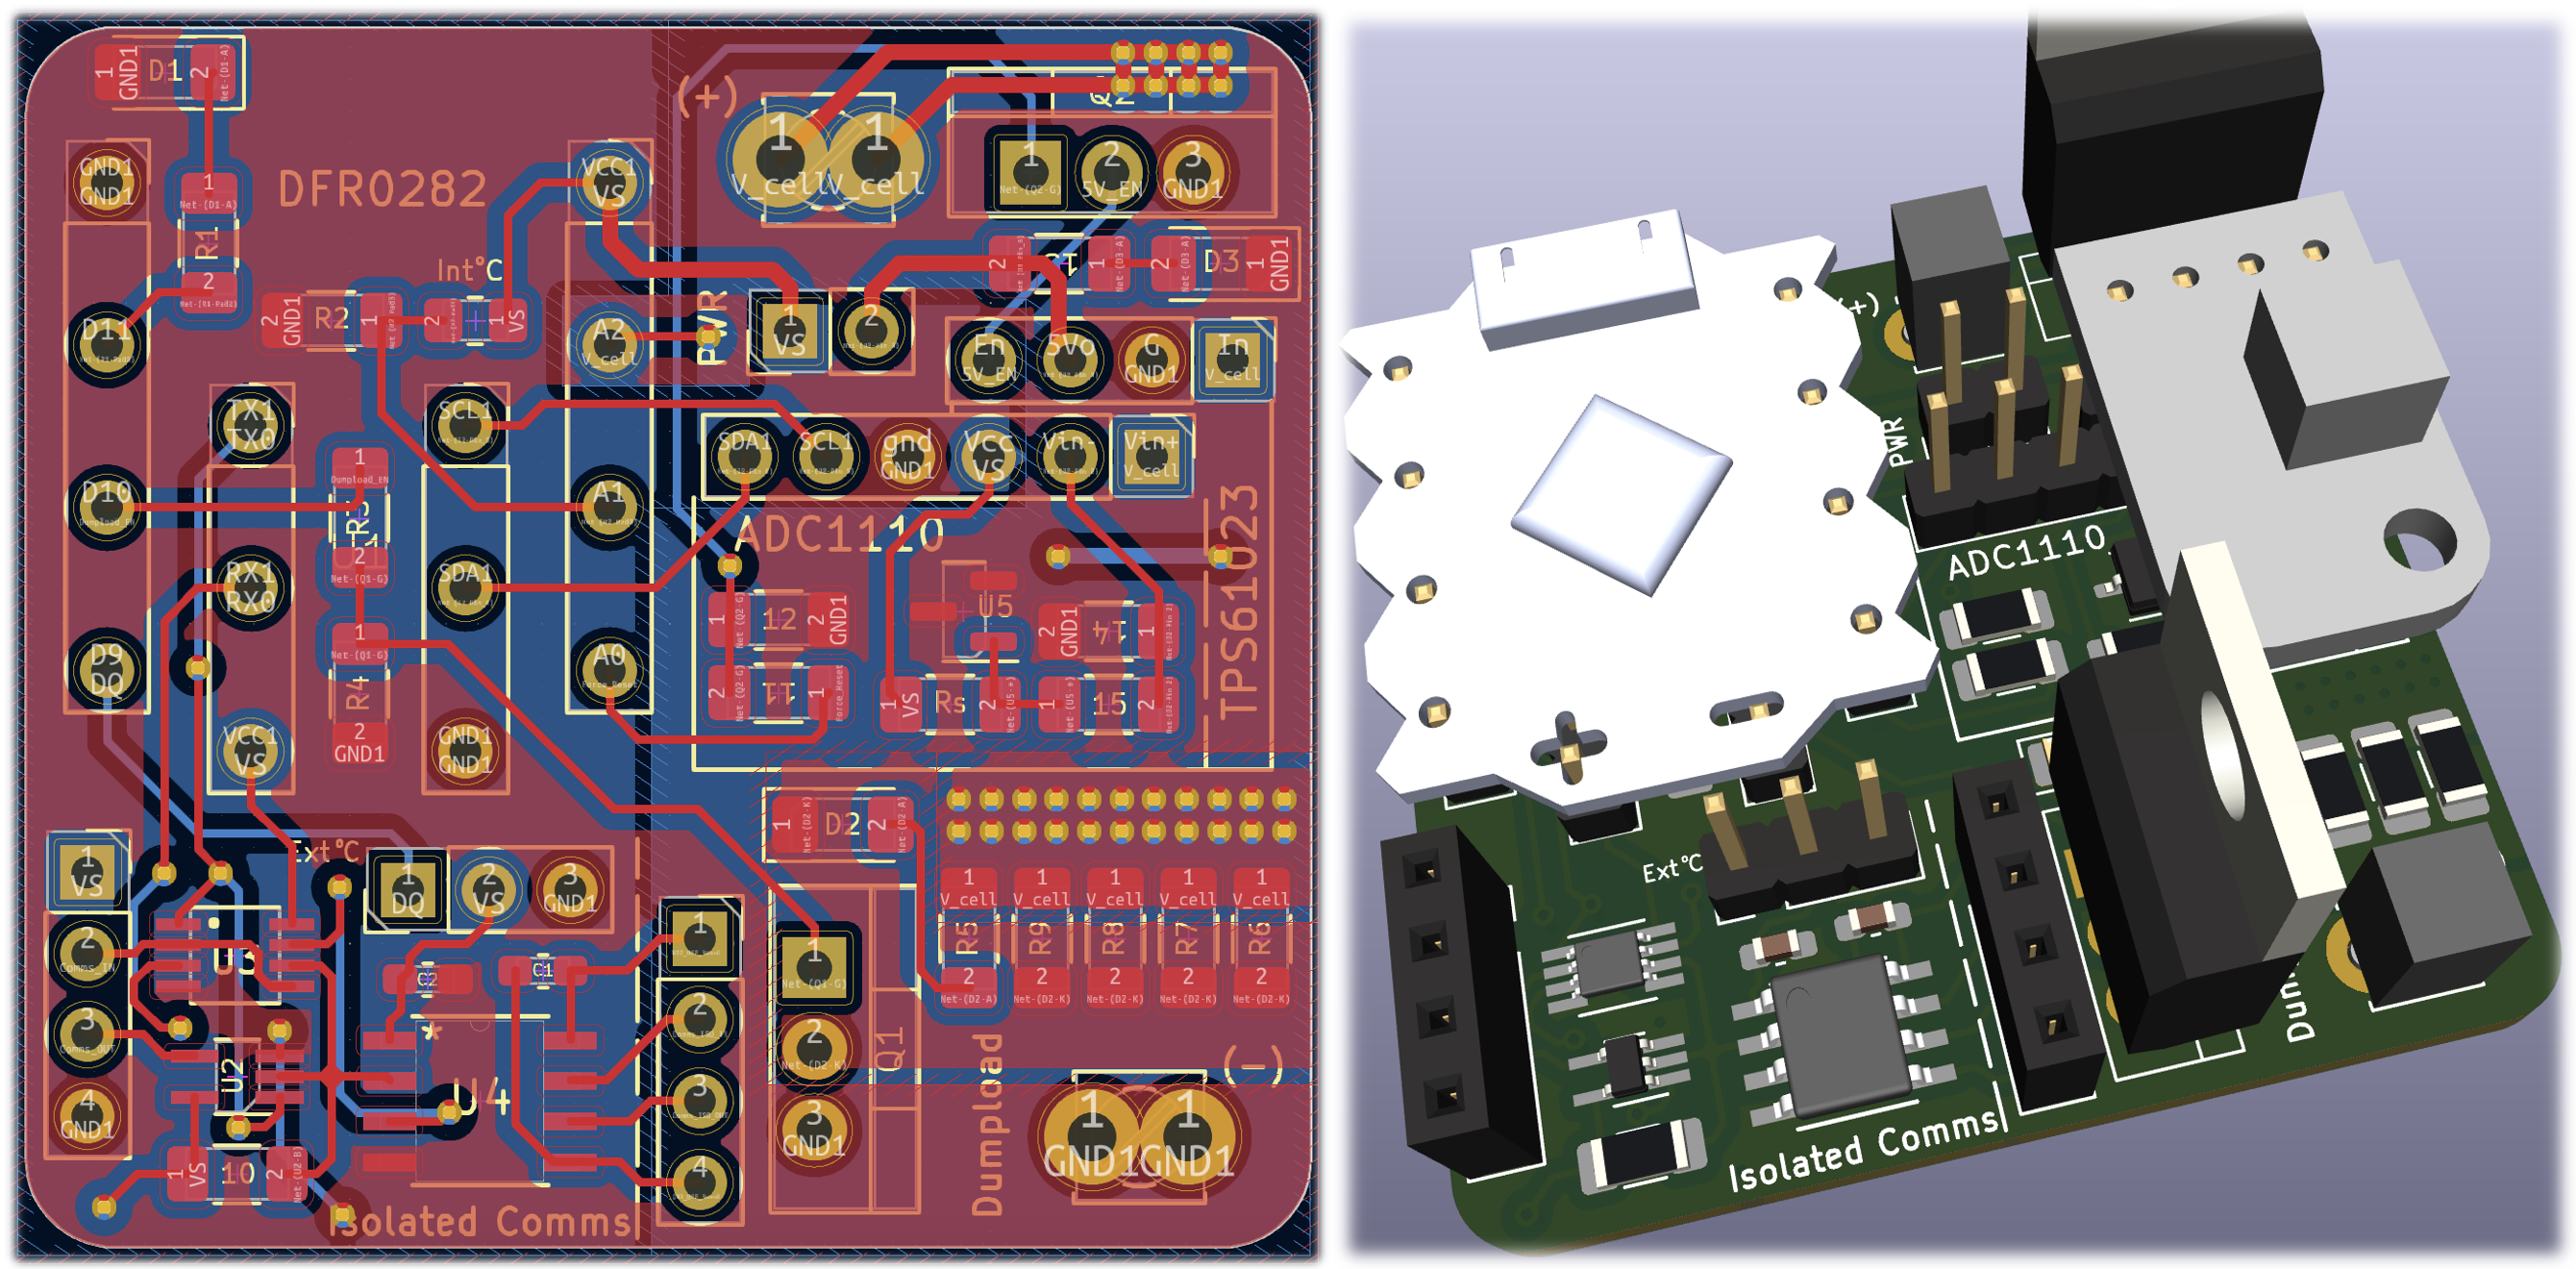
\includegraphics[width=0.77\textwidth]{Skripsie_LaTeXTemplate/Figures/MonitorPCB.png}
\caption{KiCad Software Monitoring Module Design \cite{ki}}
\label{fig:Monitoring_Board_PCB_2D}
\end{figure}
\newpage
%#####################################################################################################
\section{Master Controller Design}\label{subsec:mstr_contt}
%########################################################
\subsubsection{Design Outline}\label{subsec:mmmm4}
%########################################################
The main controller, serving as the master device in the communication system, solely monitors the current flowing into or out of the battery bank, while other battery parameters are relayed to it. It conducts real-time analysis to determine the connectivity of the battery to the load/charger, processes, and logs the data, primarily aiming to ensure battery safety and manage the state of cells within the battery bank. A meticulous inspection of the circuit design and component selection for each subsystem on the master controller board is delineated in the following section, with the PCB design further substantiating the system's compliance with the design requisites for power line control.

\begin{figure}[h!]
\centering
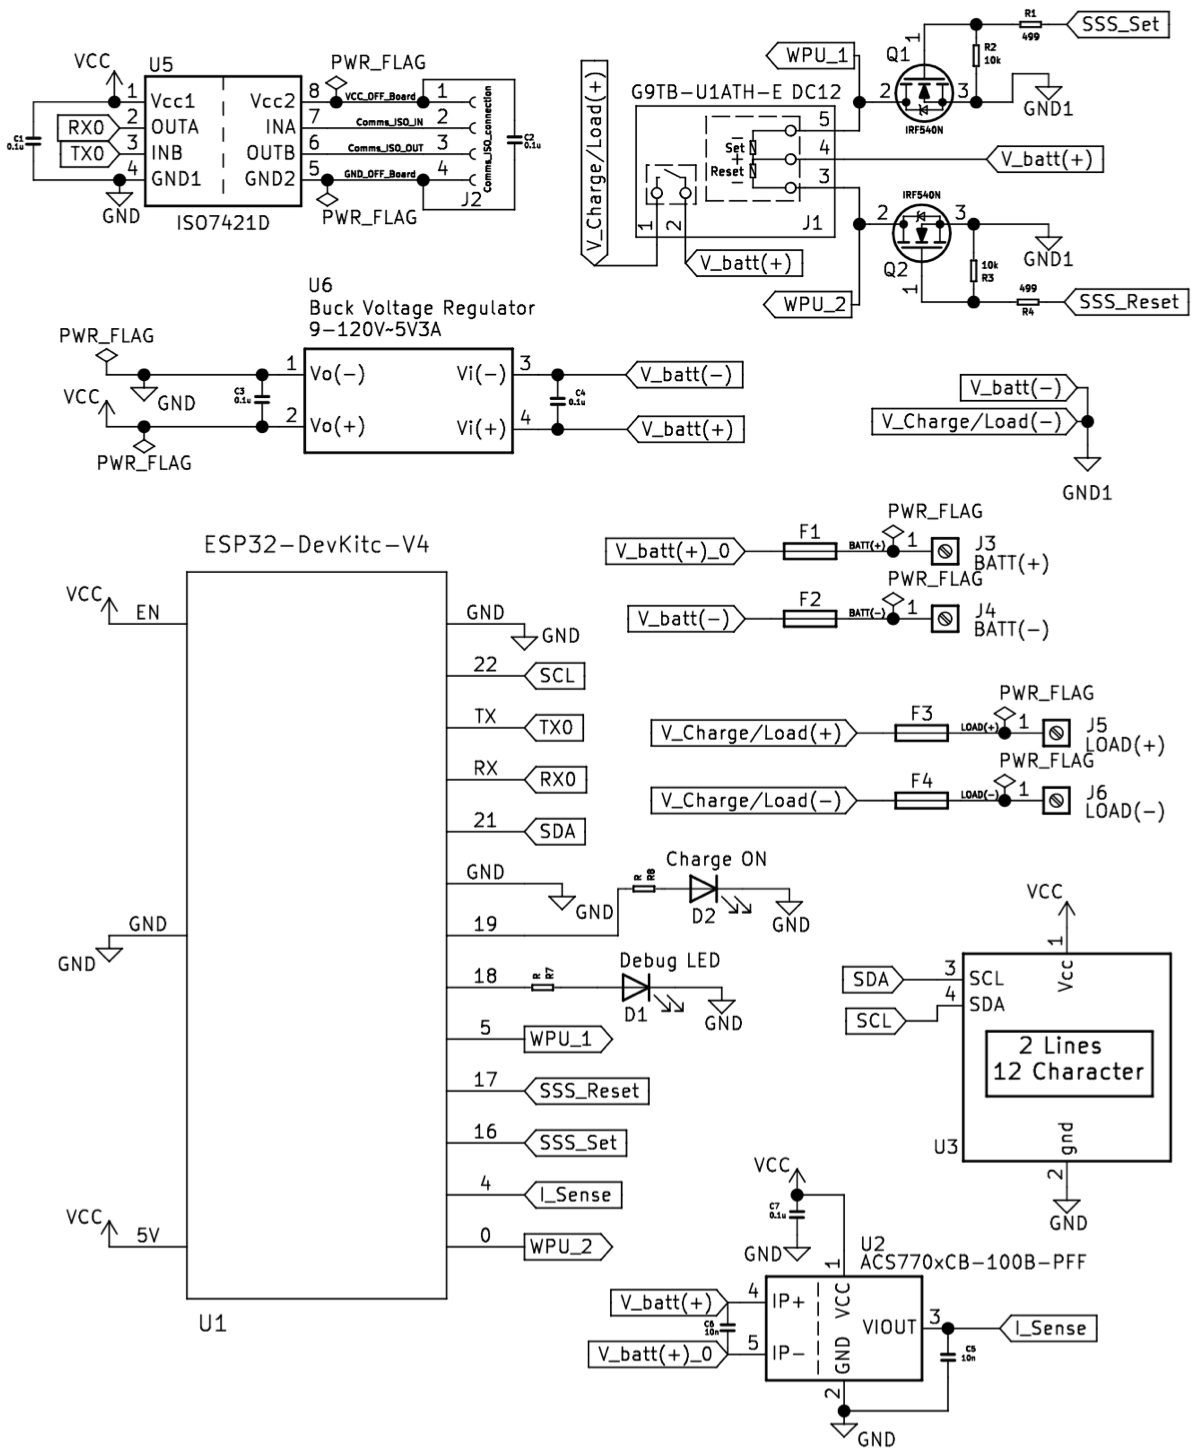
\includegraphics[width=0.82\textwidth]{Skripsie_LaTeXTemplate/Figures/Mstr_Schematic.png}
\caption{Main Controller Schematic Diagram}
\label{fig:Mstr_Schema}
\end{figure}
\newpage
%########################################################
\subsubsection{Circuit Designs \& Component Selection}\label{subsec:mmmm5}
%########################################################
\textbf{\emph{Terminals \& Fuse Protection}}\label{subsubsec:mstr_terminals_dsgn}

\begin{figure}[h!]
\centering
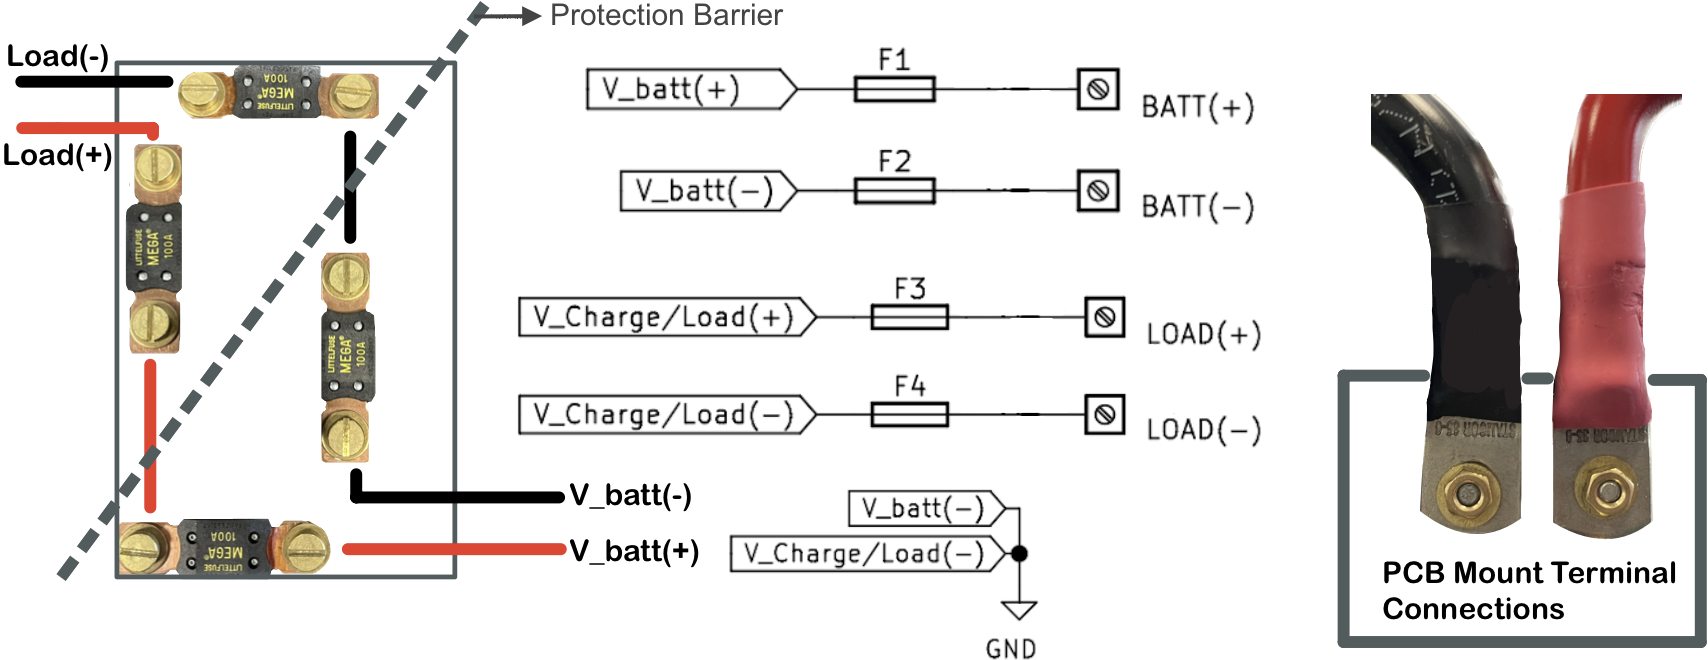
\includegraphics[width=0.7\textwidth]{Skripsie_LaTeXTemplate/Figures/Terminals_Fuses_DesigN.png}
\caption{Power Line Isolation \& Connections \cite{BigFuse}}
\label{fig:Mstr_D6}
\end{figure}
\noindent
Figure \ref{fig:Mstr_D6} illustrates the interconnection of the positive and negative lines of a battery pack and a load/charger via 130A PCB mount through hole screw terminals from Würth Elektronik \cite{BigTerminal}. To enhance safety, the controller employs 100A fuses \cite{BigFuse} on both lines, achieving complete isolation between the battery pack and the load/charger. This dual fusing strategy is essential in high voltage DC systems for mitigating risks associated with insulation failure that could lead to line-to-line DC short-circuit fault conditions. In a controlled setup like this power line control board, such fusing on both sides of the circuit safeguards the system against overcurrent conditions, thereby bolstering the reliability and safety of the control system. The incorporation of 100A fuses on both lines aligns with the best practices in high voltage DC system design, demonstrating a diligent approach to safety and protection.\newline\newline
%########################################################
\noindent
\textbf{\emph{Power Supply}}\label{subsubsec:mstr_Supp}\newline
\noindent
The choice of employing the Buck Voltage Regulator VIN 9-120V VOUT 5V3A \cite{12Vto5V} is dictated by the necessity for a stable 5V reference to power the control circuitry on the master board, similar to the monitoring module. For high scalability in the battery pack, this regulator provides a voltage range of 9V to 120V. This regulator not only caters to the maximum current demand of the system but also offers a surplus, ensuring a reliable power supply. The 5V logic level derived from this regulator facilitates a high resolution range, crucial for achieving precision in measurement processing within the system.\newline

\begin{figure}[h!]
\centering
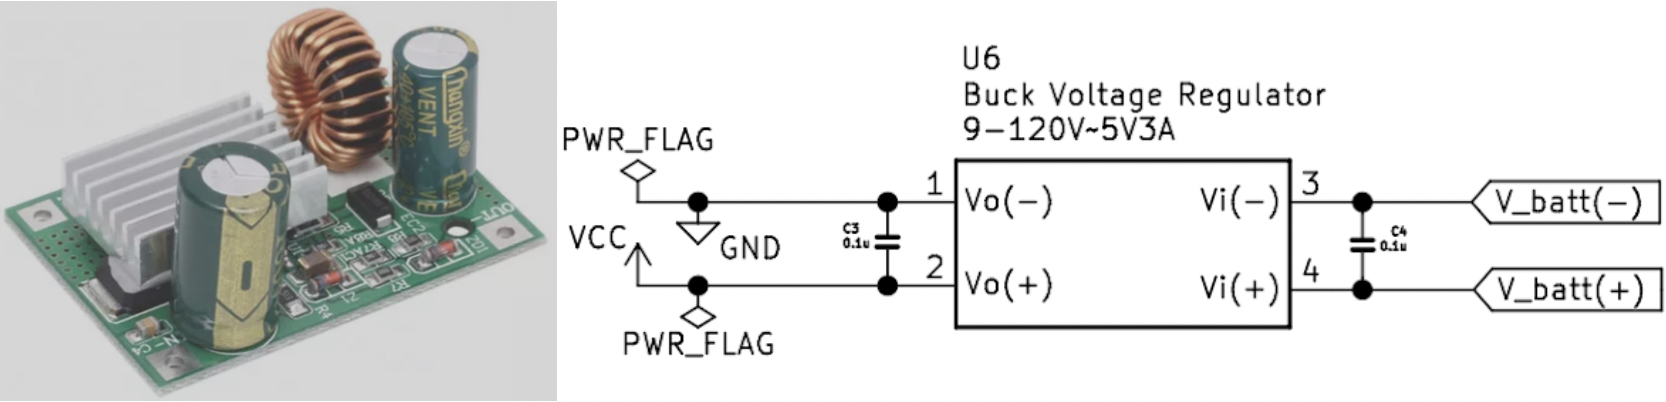
\includegraphics[width=0.7\textwidth]{Skripsie_LaTeXTemplate/Figures/P_Sup_DesigN.png}
\caption{Buck Voltage Regulator \cite{12Vto5V}}
\label{fig:Mstr_D5}
\end{figure}
\newpage
%########################################################
\noindent
\textbf{\emph{Master Microcontroller}}\label{subsubsec:ESP32_dsgn}\newline
\noindent
The ESP32 DevKitC V4 microcontroller by Espressif \cite{The_ESP_ref} is tailored for system controller applications, demonstrating adept handling of UART communication protocols for real-time interaction with slave monitoring devices. It processes data from series string cells efficiently and uploads it to the cloud via integrated Wi-Fi functionality, enabling real-time monitoring and system analysis.

\begin{figure}[h!]
\centering
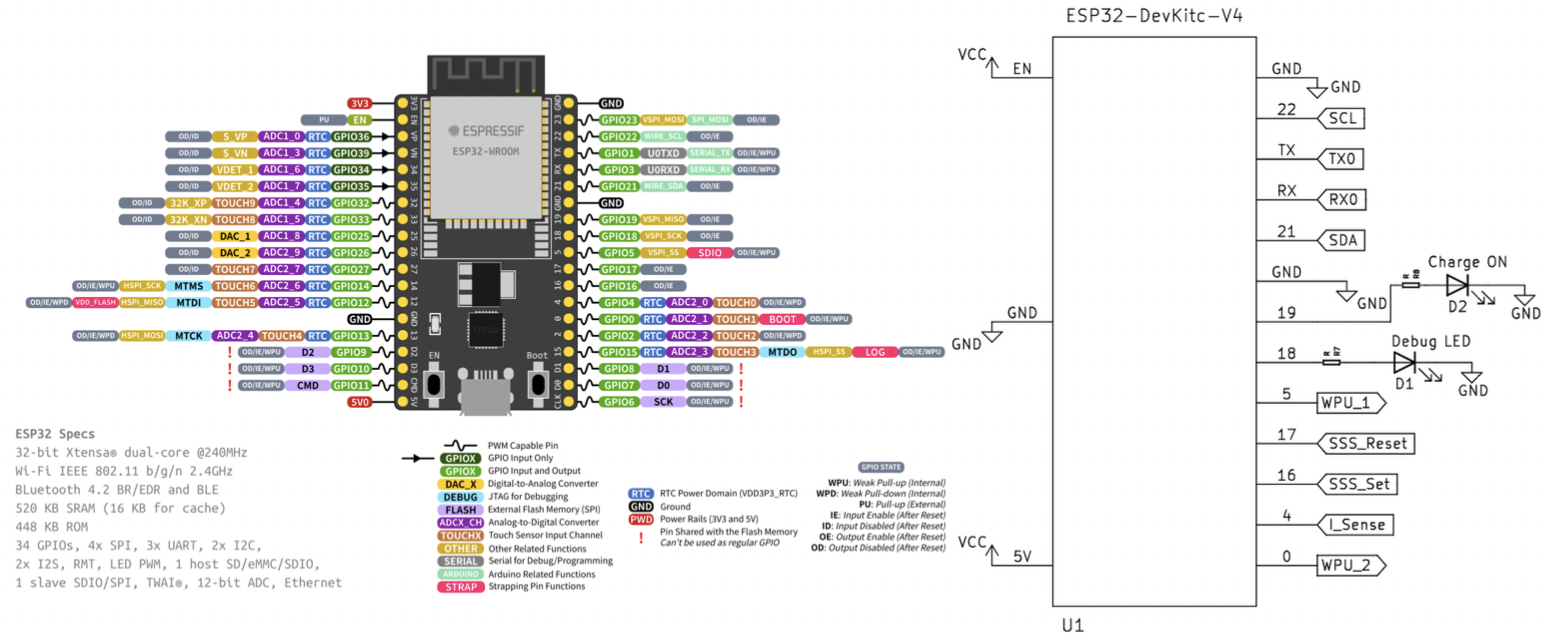
\includegraphics[width=1.0\textwidth]{Skripsie_LaTeXTemplate/Figures/The_ESP_DesigN.png}
\caption{ESP32DevKitCv4 Master Microcontroller \cite{The_ESP_ref}}
\label{fig:Mstr_D4}
\end{figure}
\noindent
This microcontroller is cost-effective compared to alternatives like the Raspberry Pi, yet provides a rich feature set. The on-board Wi-Fi ensures real-time data transmission and remote monitoring. Its compatibility with Arduino IDE facilitates effortless interfacing with DFR0282 slave modules for cell monitoring, simplifying development and accelerating deployment of monitoring and control logic. The ESP32 DevKitC V4 is mounted on the master controller board, featuring an on-board micro-USB port for program updates. Below is a table detailing the pin configurations and utilities on the master controller board.

\begin{table}[h]
    \centering
    \caption{Master Microcontroller Pin Out}
    \label{tab:ESP_PinOut}
    \begin{tabular}{|c|c|c|c|}
        \hline
        \textbf{ESP32-Pin} & \textbf{Name} & \textbf{Configuration} & \textbf{Utility} \\
        \hline
        \hline
        3 & IO22 & Arduino Wire-Lib SCL & I2C clock for LCD \\
        \hline
        4 & TX & UART Protocol & Serial transmit channel \\
        \hline
        5 & RX & UART Protocol & Serial recieve channel \\
        \hline
        6 & IO21 & Arduino Wire-Lib SDA & I2C data for LCD \\
        \hline
        8 & IO19 & Digital Output & Charge/Load ON indication \\
        \hline
        9 & IO18 & PWM Channel & System debug messages LED \\
        \hline
        10 & IO5 & GPIO State & Internal weak pull-up 1 \\
        \hline
        11 & IO17 & Digital Pulse & Lacthing relay RESET \\
        \hline
        12 & IO16 & Digital Pulse & Lacthing relay SET \\
        \hline
        13 & IO4 & Analog Channel & Current sensor input \\
        \hline
        14 & IO0 & GPIO State & Internal weak pull-up 2 \\
        \hline
    \end{tabular}
\end{table}
\newpage
%########################################################
\noindent
\textbf{\emph{Battery Current Measurement}}\label{subsubsec:cur_sen_design}\newline
\noindent
The ACS770LCB-100B current sensor from Allegro Microsystems \cite{currentSensori} is utilized to measure the current flowing from the battery's positive terminal to the load/charger. Accompanying the sensor are a $0.1 \mu F$ decoupling capacitor between its 5V supply lines, a $10 nF$ bypass capacitor at its output, and another $10 nF$ capacitor between the current path's positive and negative terminals for noise mitigation. The sensor's output delivers a voltage signal representative of the battery pack's current to the microcontroller, within a measurement range of -100A to 100A and a corresponding output voltage range of 0V to 5V.\newline\newline
\noindent
The linear transfer characteristic of the sensor is given by the formula below.
\[ V_{out} = V_{zero} + (S \cdot I) \]
\noindent
Where \(V_{zero} = 2.5V\) (sensor output at zero current) and \(S\) the sensitivity, is calculated.
\[ S = \frac{5V}{200A} = 0.025 \, \text{V/A} \]
\noindent
The accuracy of the measurement is evaluated considering a sensor accuracy specification of $0.5\%$. For a measured current of $50A$, the error and its corresponding voltage error are calculated as follows:
\begin{equation}
\label{eq:I_error}
\text{Error} = 0.5\% \cdot 50A = 0.25A
\end{equation}
\begin{equation}
\label{eq:V_error}
V_{\text{error}} = 0.025 \, \text{V/A} \cdot 0.25A = 0.00625V
\end{equation}

\begin{table}[h]
    \centering
    \caption{Sensor Voltage Output for Various Current Values}
    \label{tab:Sensor_Output}
    \begin{tabular}{|c|c|c|}
        \hline
        \textbf{Current (\(I\))} & \textbf{Expression} & \textbf{Output Voltage (\(V_{out}\))} \\
        \hline
        50A & \(2.5V + (0.025 \, \text{V/A} \cdot 50A)\) & 3.75V \\
        \hline
        -50A & \(2.5V + (0.025 \, \text{V/A} \cdot -50A)\) & 1.25V \\
        \hline
        100A & \(2.5V + (0.025 \, \text{V/A} \cdot 100A)\) & 5V \\
        \hline
    \end{tabular}
\end{table}

\noindent
The design, shown in figure \ref{fig:Mstr_D1}, leverages the ACS770LCB-100B to translate battery current to a voltage signal for microcontroller interpretation, with capacitors employed for noise suppression, thus bolstering system reliability and measurement accuracy.

\begin{figure}[h!]
\centering
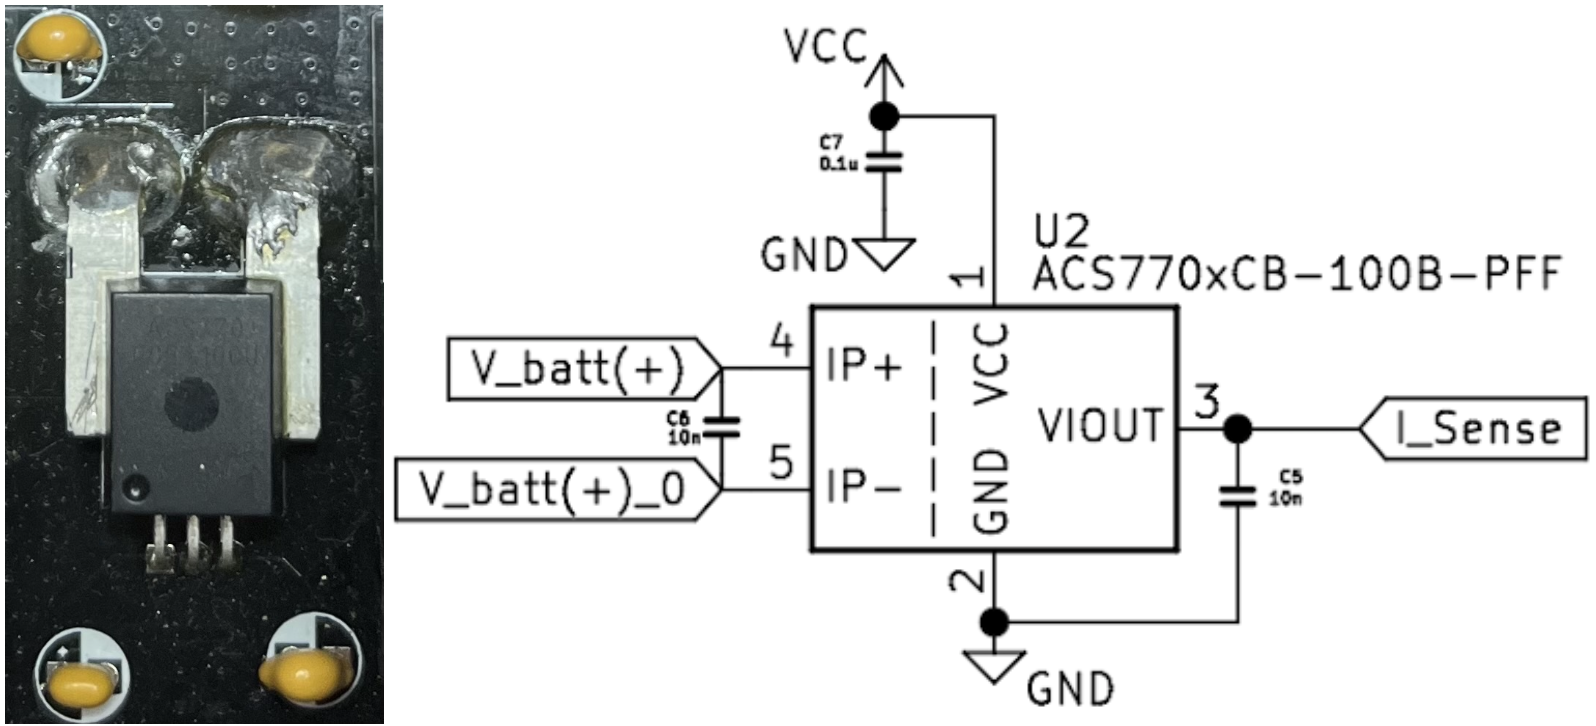
\includegraphics[width=0.5\textwidth]{Skripsie_LaTeXTemplate/Figures/Cur_Sen_DesigN.png}
\caption{Battery Cerrent Sensor \cite{currentSensori}}
\label{fig:Mstr_D1}
\end{figure}
\newpage
%########################################################
\noindent
\textbf{\emph{System Information Display}}\label{subsubsec:LCD_Dsgn}\newline
\noindent
The generic LCD 16x2 Character Display, White on Blue Background, 5V, along with the I2C Interface Module for LCD, 3.3/5V Ready, from Microrobotics \cite{LCD_MR}, are integrated on the control board. This setup facilitates communication between the microcontroller and the LCD via the I2C protocol. The I2C Interface Module simplifies the connection requiring only four wires: VCC, GND, SDA, and SCL. Through this setup, the microcontroller can dispatch summarized system messages to the LCD, providing a succinct insight into the state of system variables, ensuring a user-friendly interface for real-time system monitoring.

\begin{figure}[h!]
\centering
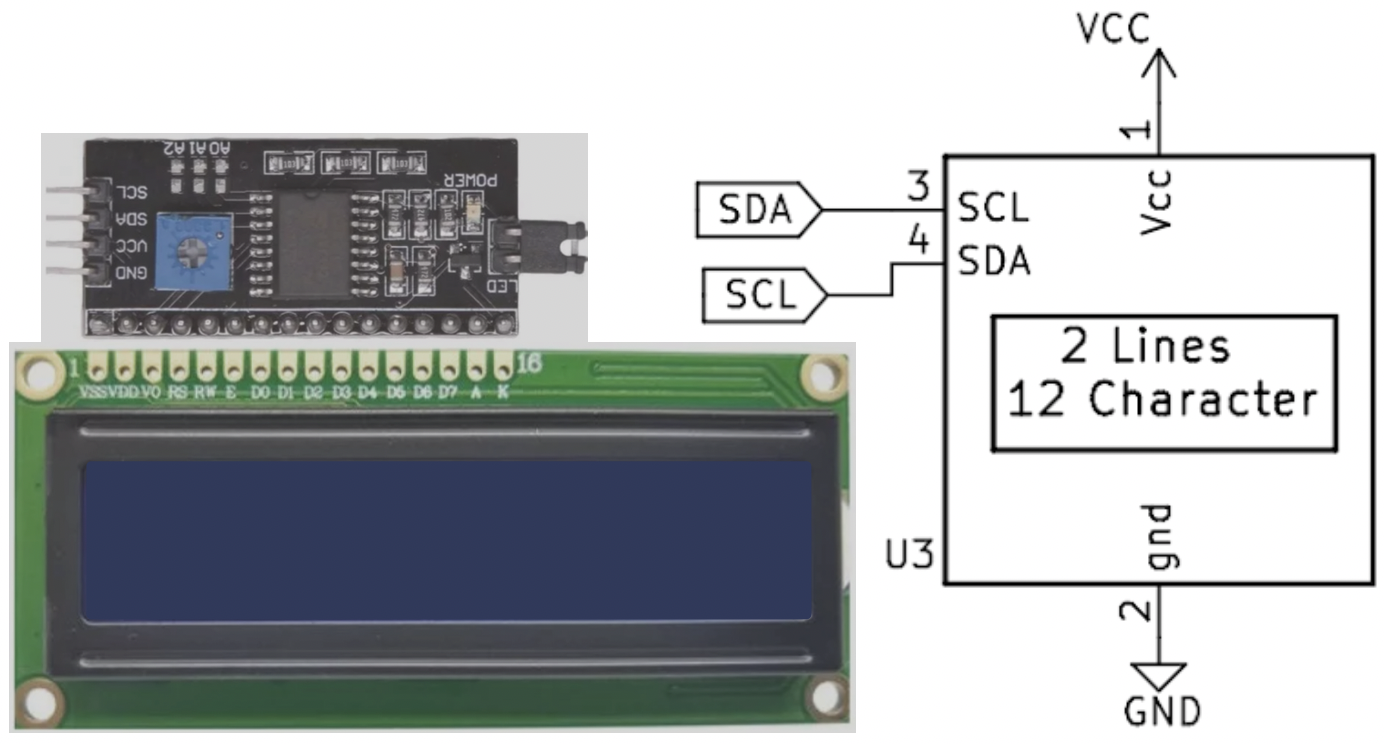
\includegraphics[width=0.36\textwidth]{Skripsie_LaTeXTemplate/Figures/The_LCD_DesigN.png}
\caption{LCD with I2C Module \cite{LCD_MR}}
\label{fig:Mstr_D3}
\end{figure}
%########################################################
\noindent
\textbf{\emph{Load/Charge Disconnect}}\label{subsubsec:relay_Dsgn}\newline
\noindent
The Omron G9TB-K1ATH-E DC12 relay, positioned in series between the battery pack and the load/charger, serves as a switch for power flow, safeguarded by fuse protection on both sides for a maximum current of 100A.

\begin{figure}[h!]
\centering
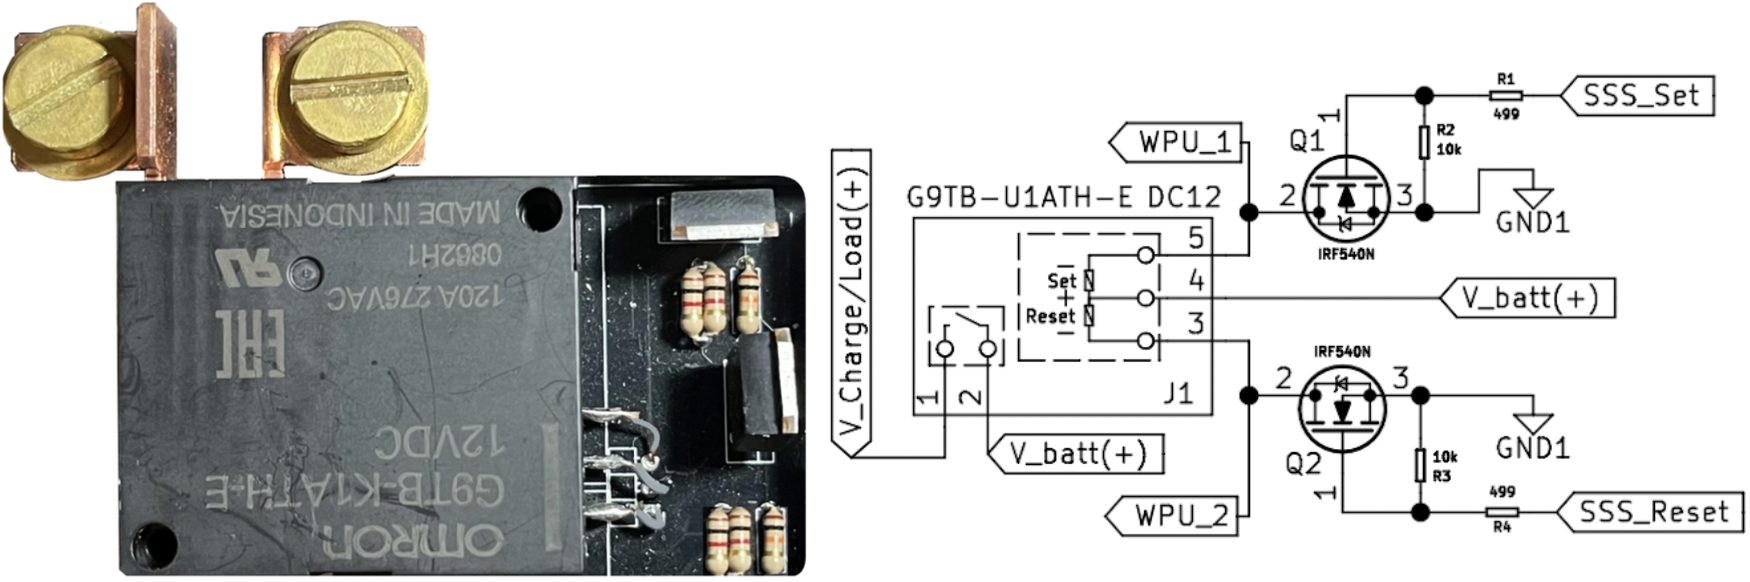
\includegraphics[width=0.7\textwidth]{Skripsie_LaTeXTemplate/Figures/Relay_DesigN.png}
\caption{Latching Power Relay \cite{RELAY}}
\label{fig:Mstr_D7}
\end{figure}
\noindent
The relay requires a 12V amplitude pulse for state transition, yet the ESP32 microcontroller outputs a maximum amplitude pulse of 5V. To bridge this voltage gap, external circuitry, depicted in figure \ref{fig:Mstr_D7}, is designed. Two identical MOSFETs from the dump-load circuits of the cell monitoring modules are integrated in low-side switch configurations, simplifying the design for gate limiting and pull-down resistors as per subsubsection \ref{subsubsec:LS_SW}.\newline\newline
\noindent
The gates of these MOSFETs are connected to distinct microcontroller pins labeled SET and RESET, enabling a 25ms pulse for the relay's operation. The common pin of the relay coils is tied to the positive battery voltage (12V), while the set and reset pins on the relay are linked to a MOSFET's drain pin and an internal pull-up pin of the microcontroller, ensuring the relay pins float high when MOSFETs are non-conductive.\newline\newline
\noindent
The source pins of each MOSFET are connected to the negative battery voltage (0V), enabling a 12V potential across the relay's set or reset coil upon a 5V, 25ms pulse from the microcontroller. A hardcoded protocol in the microcontroller ensures that SET and RESET pins are not pulsed concurrently, preventing erroneous relay actuations.
\newline\newline
%########################################################
\noindent
\textbf{\emph{Scalable Isolated Communication}}\label{subsubsec:iso_COMS_Mstr}

\begin{figure}[h!]
\centering
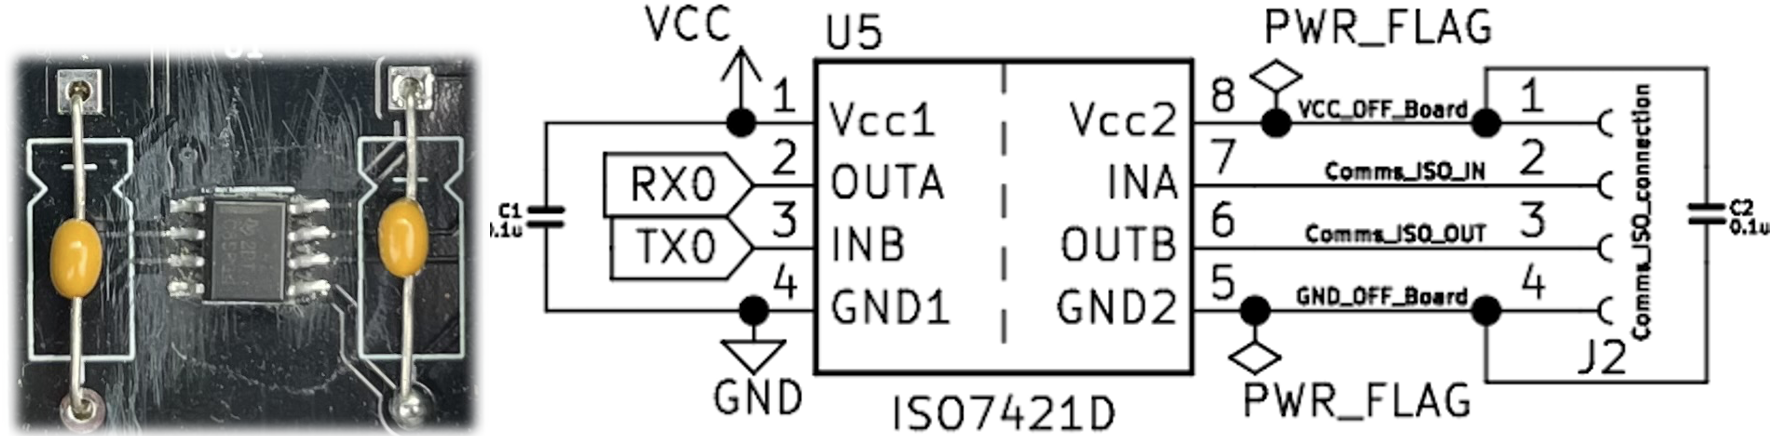
\includegraphics[width=0.4\textwidth]{Skripsie_LaTeXTemplate/Figures/Mstr_Comms_DesigN.png}
\caption{Master Controller Isolated Communication}
\label{fig:Mstr_D2}
\end{figure}
\noindent
The master controller's communication lines are isolated using the ISO7421D chip, identical to the one used in the cell monitoring modules as referenced in subsubsection \ref{subsubsec:iso_COMS}. Being at the start of the communication line, the master device is shielded against bus contention by the logic circuit on the first slave device in the stack.
%########################################################
\subsubsection{Printed Circuit Board Design}\label{subsec:mmmm6}
%########################################################
\begin{figure}[h!]
\centering
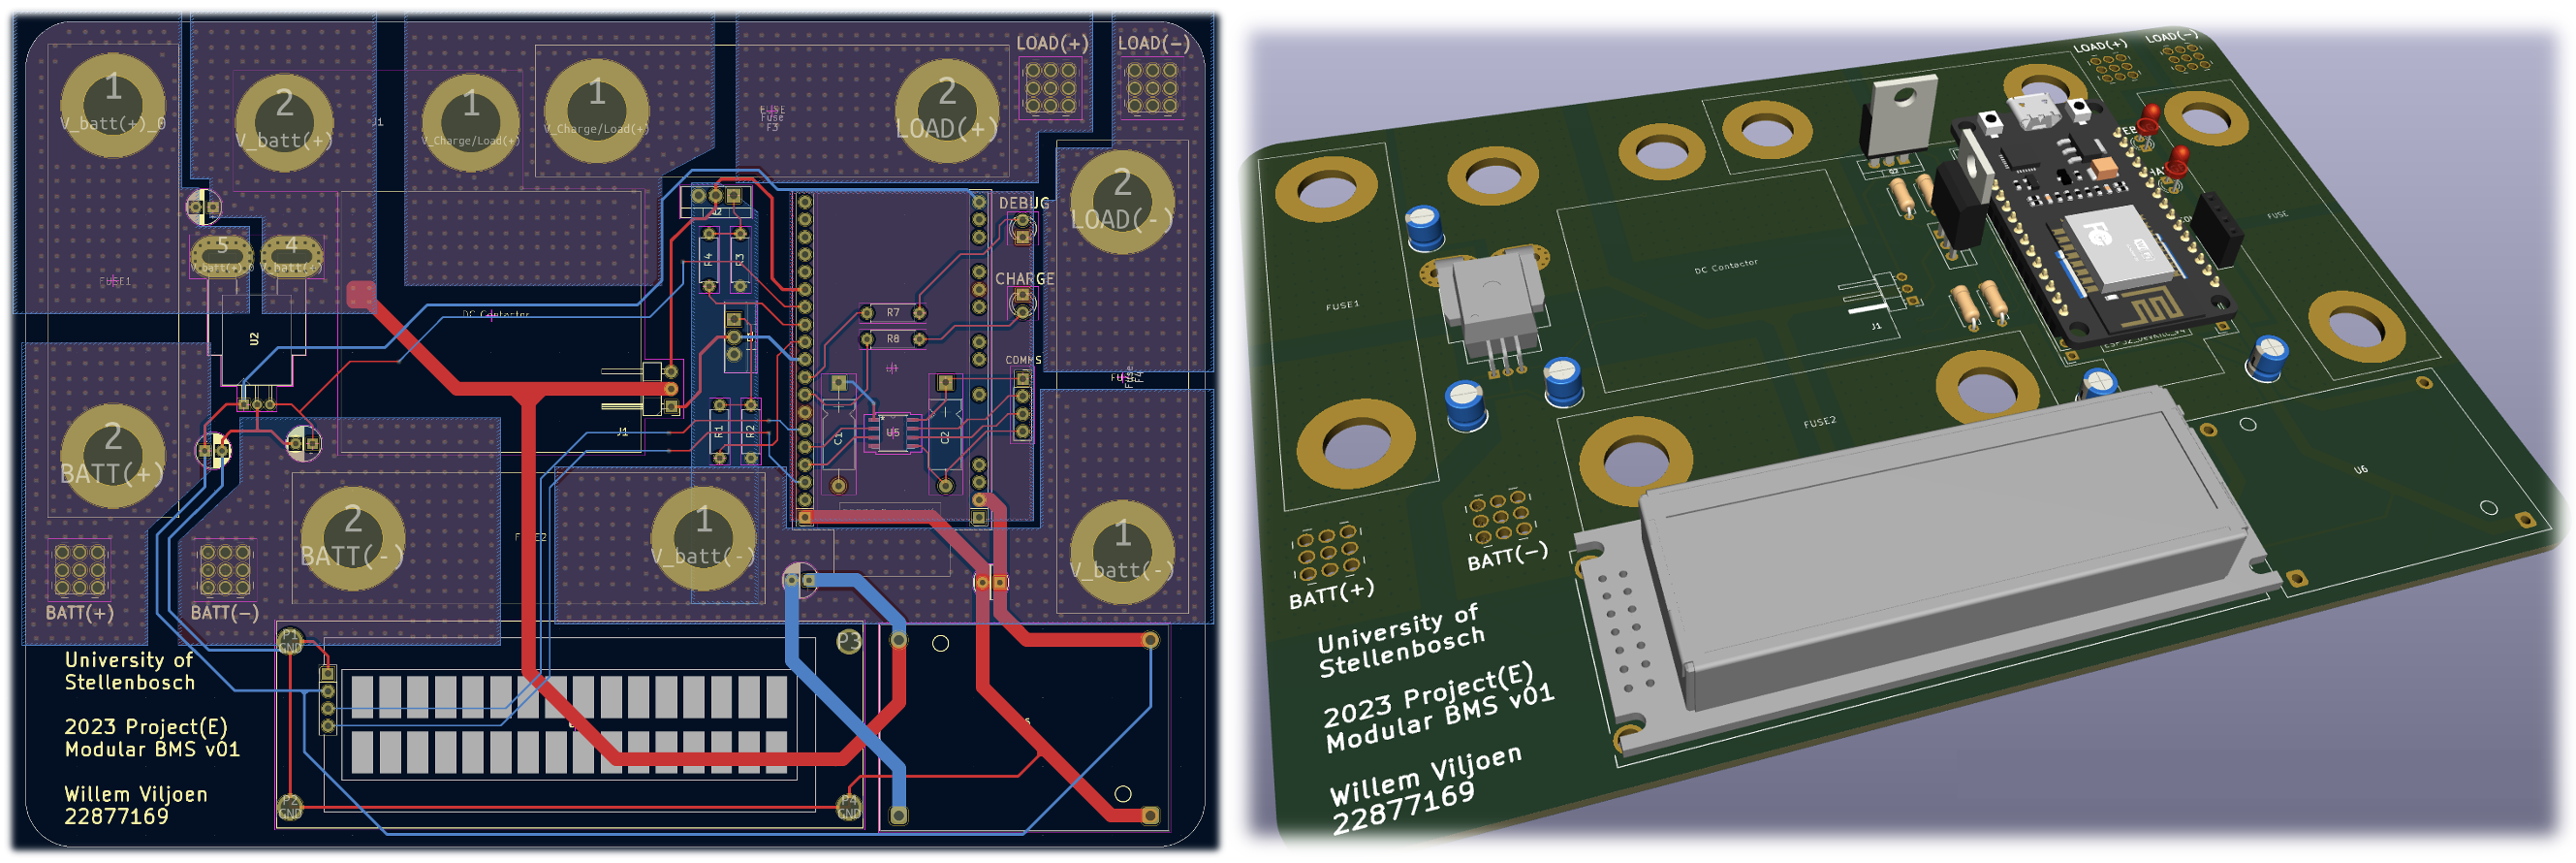
\includegraphics[width=0.94\textwidth]{Skripsie_LaTeXTemplate/Figures/ControllerPCB.png}
\caption{KiCad Software Master Controller Design}
\label{fig:Master_Board_PCB_2D}
\end{figure}
\noindent
In the figure above, the left illustrates the PCB design, showcasing all copper layers and component footprints selected during the design process of the master controller board. To accommodate a high current of 120A on the battery power lines flowing through the master controller board, filled copper layers and via stitching techniques were employed. These design approaches enhance the current-carrying capacity and thermal management of the PCB. A thermal test for the current capability of the master controller board is slated for evaluation in Section \ref{sec:systEVAL}. As depicted on the right, the design successfully integrates a 3D representation of the board, fitting perfectly to the side of the first cell in the series stack at the battery bank's input/output. Refer to Appendix \ref{appen:cad} for the complete CAD assembly design.
\newpage
%########################################################
\section{Design Review}\label{subsec:Des_Review}
%########################################################
The diagram below succinctly illustrates the system solution for \emph{a Modular Battery Management System for LFP Batteries}, showcasing the independent yet compatible monitoring modules and the master controller. These units, while autonomous, are interconnected through a communication network to form a cohesive BMS ecosystem for a battery bank. The design underscores the synergy between the controller, cell modules, and communication system, functioning both individually and collectively to ensure system integrity.

\begin{figure}[h!]
\centering
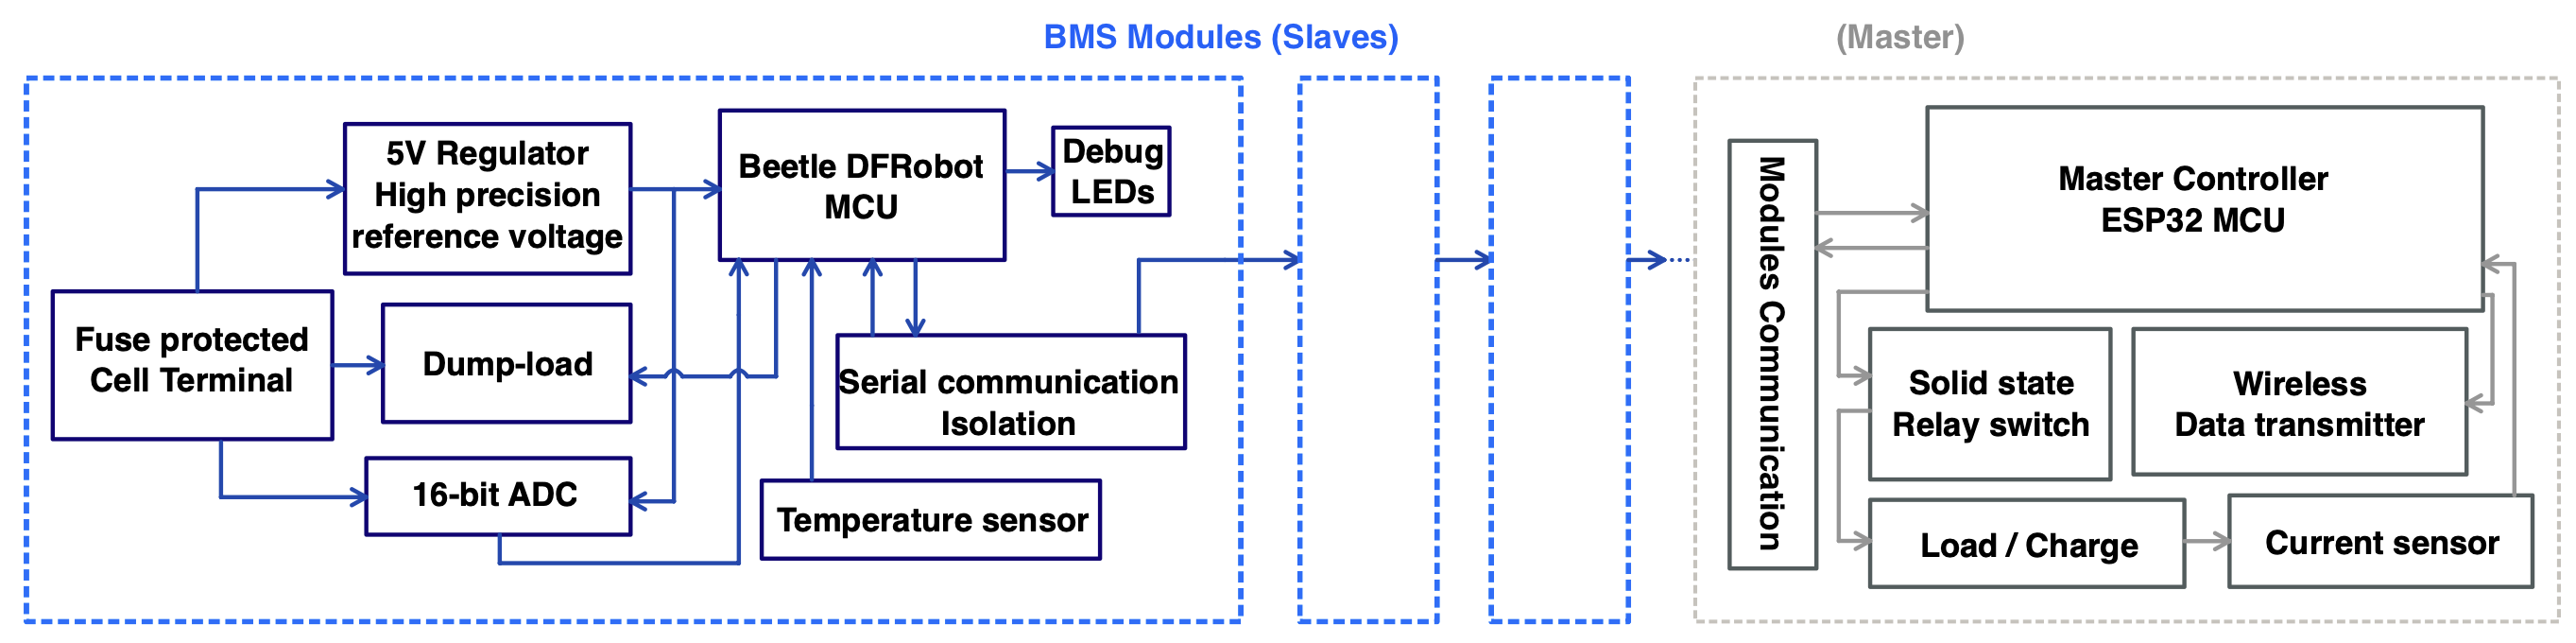
\includegraphics[width=1.0\textwidth]{Skripsie_LaTeXTemplate/Figures/setup.png}
\caption{Complete System Design}
\label{fig:setup_dsgn}
\end{figure}
\noindent
The modular BMS topology features cell-level monitoring modules and a central controller, marking a significant evolution in energy management. It achieves precise, real-time data collection and enhances system-wide awareness. Embedded microcontrollers within each module process data locally, reducing latency and improving accuracy, which simplifies the system's complexity and improves reliability.\newline\newline
\noindent
The central controller is pivotal, managing data flow and system communications with a focus on power control and resilient PCB design. It synthesizes cell data, supporting informed energy management decisions. In sum, the BMS melds modular design with centralized oversight, offering scalability and adaptability to meet evolving battery management needs, and is poised to set new industry benchmarks.\newline\newline
\noindent
\textbf{\emph{Design Tools Acknowledgment:}}\newline
\noindent
The subsequent figure presents a curated selection of icons representing the sophisticated design and development software applications instrumental to the engineering and design processes of this project.

\begin{figure}[h!]
\centering

\includegraphics[width=0.9\textwidth]{Skripsie_LaTeXTemplate/Figures/icons.png}
\caption{Design Software Packages}
\label{fig:DSP}
\end{figure}

\vfill

\chapter[System Evaluation]{Chapter 5: System Evaluation}\label{chap:before_last}
%########################################################
\section{Design Outcomes}\label{sec:DO_}
%########################################################
The design review, constrained by the timing of PCB and component procurement and subsequent prototyping, served primarily as a reference for future enhancements rather than immediate project revisions, aligning with the limitations outlined in the \hyperref[sec:drawbacks]{Hypotheses \& Potential Drawbacks} section. The prototype and debugging phases surfaced several design outcomes, including both the successful implementation of subsystem designs and an identified critical flaw: the malfunction of the UART communication between cell monitoring modules.\newline\newline
\noindent
The communication issue originated from the complex hardware interactions within the Arduino Beetle (DFR0282) microcontrollers, particularly affecting the hybrid daisy-chain serial communication setup. The challenges included maintaining a stable 16 MHz clock for precise UART timing, implementing effective flow control, and ensuring accurate pin configuration. These factors, both individually and collectively, compromised the UART system, as further detailed through exhaustive debugging and analysis.\newline\newline
\noindent
Despite this setback, the communication hardware was independently verified as functional, isolating the issue to the microcontrollers used. All other systems and subsystems performed optimally and will be discussed in this chapter. Chapter \ref{chap:last} will propose future actions for multi-module communication and alternative microcontroller recommendations for the cell monitoring boards.
%########################################################
\section{Valuation Prospect}\label{sec:prospect}
%########################################################
This chapter presents a thorough evaluation of the designed modular Battery Management System, ensuring subsystem compliance with key performance and safety standards. We will conduct exhaustive testing of each subsystem in simulated operational environments to verify performance within optimal thresholds. Tests include electrical, thermal, and fault response assessments to establish reliability, state-of-charge accuracy, and overall system integrity. Additionally, we will analyze performance under variable load conditions to evaluate module adaptability and robustness. Our systematic evaluation aims to provide a detailed understanding of subsystem operation and integration within the BMS, guaranteeing cohesive operation, battery longevity, and user safety upon final assembly. This strategy underpins the BMS's integrative success by confirming the efficacy of individual subsystems.\newpage
%########################################################
\section{Prototyping}\label{sec:theProto}
%########################################################
\begin{figure}[h!]
\centering
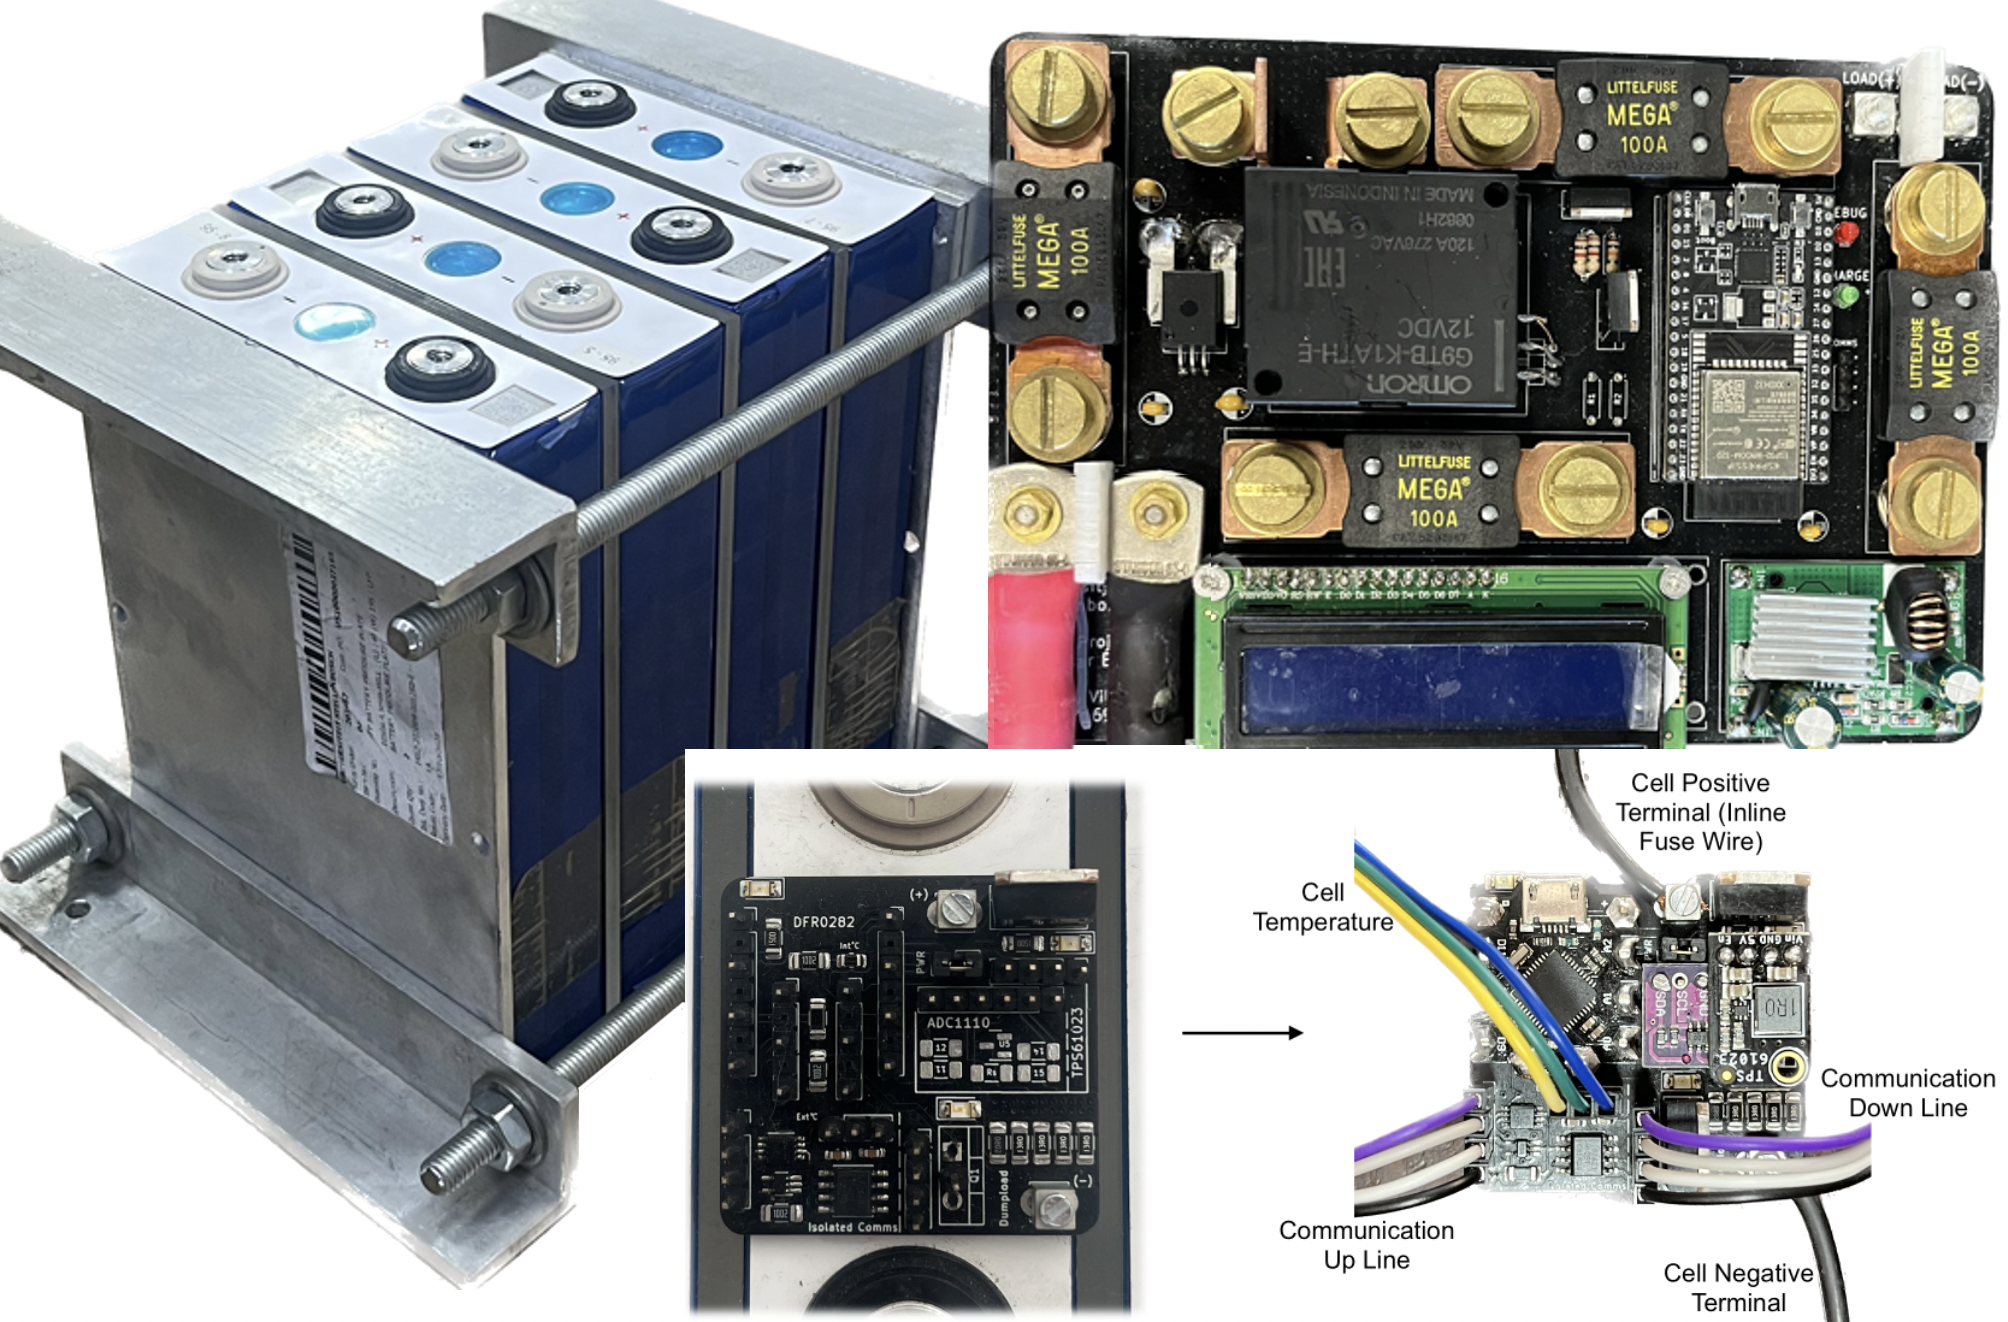
\includegraphics[width=1.0\textwidth]{Skripsie_LaTeXTemplate/Figures/proton.png}
\caption{Design \& Evaluation Prototype Builds}
\label{fig:protonn}
\end{figure}

\noindent
The provided figures showcase a constructed battery pack for experimental testing (left), an engineered main controller (top right), and a cell monitoring module prototype (bottom right). The assembly uses 100Ah 3.2V LFP cells, secured by corner profiles, threaded rods, and aluminium end plates, which, along with Perspex spacers, enforce cell compression to mitigate expansion and maintain cell integrity during discharge cycles. This technique safeguards against delamination from mechanical stress, essential for LFP cell performance. The main controller is optimized for current handling, while the monitoring modules focus on precision and compact design, serving to assess the performance of the Modular BMS systems in the project.
%########################################################
\section{Performance analysis}\label{sec:systEVAL}
%########################################################
This section elaborates on the experimental procedures conducted to assess the performance of the engineered system and its component subsystems under controlled conditions. It encompasses a description of individual tests and includes accompanying subsections that present flow diagrams, result graphs, and model configurations for a comprehensive analysis.\newpage
%*******************************************%
\subsubsection{General}\label{subsec:genZ}
%*******************************************%
The master controller and cell monitoring modules were assessed for functionality using flag-based test programs, which confirmed the onboard Debug LED system operated as intended. Calibration of the NTC sensor on the cell monitoring modules was achieved by referencing an external digital temperature sensor for internal temperature measurements. Validation of these measurements was conducted against the precise readings from a Fluke TiS20 thermal tool. Additionally, an emergency restart test was successfully executed on the cell monitoring module by transmitting a UART force reset flag, causing a momentary power loss in the microcontroller before a successful reboot.
%*******************************************%
\subsubsection{Communication Circuitry}\label{subsec:CCT}
%*******************************************%
The isolated communication system was tested utilizing an ESP32 microcontroller, wherein four GPIO pins were configured as digital outputs to simulate UART transmission (TX) for distinct cell monitoring modules. Correspondingly, four digital input pins on the ESP32 were employed to represent the reception (RX) points within the communication network, ensuring bi-directional connectivity between the microcontroller and each monitoring module's communication subsystem.

\begin{figure}[h!]
\centering
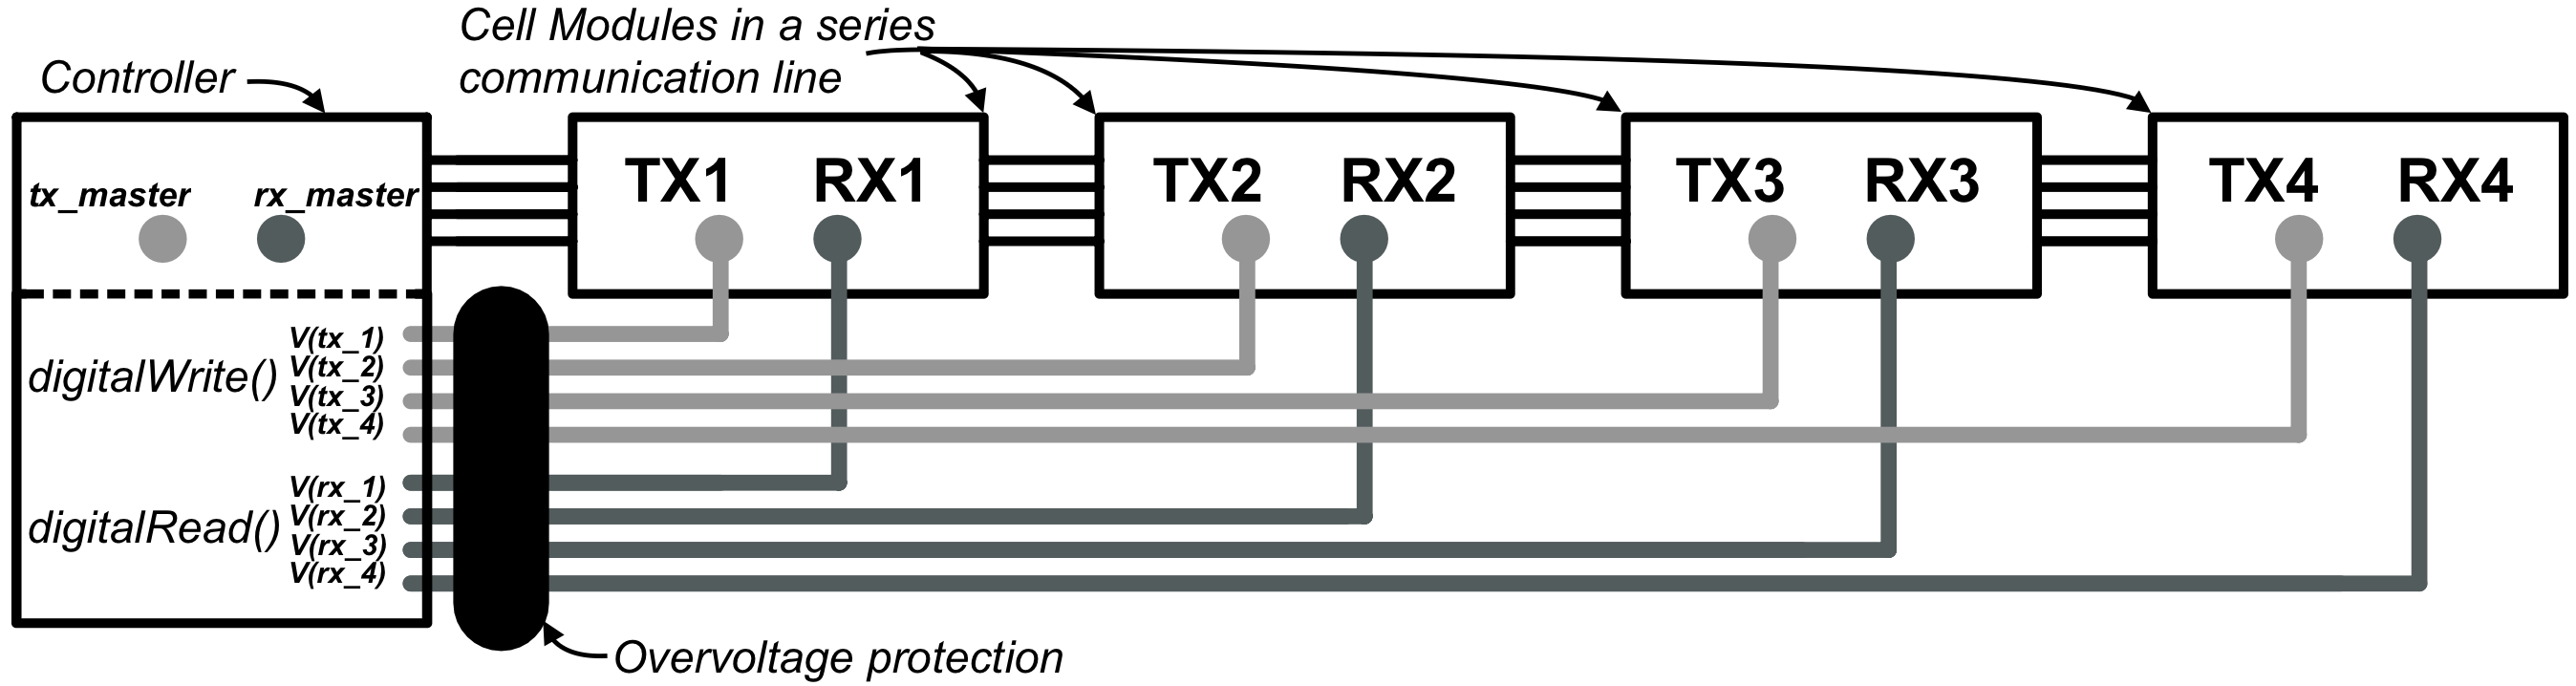
\includegraphics[width=0.75\textwidth]{Skripsie_LaTeXTemplate/Figures/theCOMMStest.png}
\caption{Communication System Test Setup}
\label{fig:comsEXP1}
\end{figure}
\noindent
Figure \ref{fig:comsEXP2} on the next page displays a serial plotter graphing both transmitted and received pulse signals. Over-voltage protection modules safeguarded the ESP32's GPIO pins, with a threshold set slightly above 5V, to mitigate bus contention risks, which didn't occur. Thus, the monitoring modules' communication circuitry operated effectively, incorporating protection logic gates that successfully prevented bus contention. This was confirmed during tests where simultaneous pulsing of two transmit pins (tx2 and tx3) occurred between 40ms and 70ms, with the received signal voltage capped at 5V. This scenario resulted in message corruption but precluded hardware damage, demonstrating the isolated communication system's resilience to potential malfunctions.\newline\newline
\noindent
It is important to note that the logic gates also serves the purpose of eliminating transmission-echo in the communication system, as we can see on the graphs now RX receives a signal transmitted from its corresponding TX. Overall, the communication circuitry integrated into each cell monitoring module functioned as expected.
\newpage
\begin{figure}[h!]
\centering
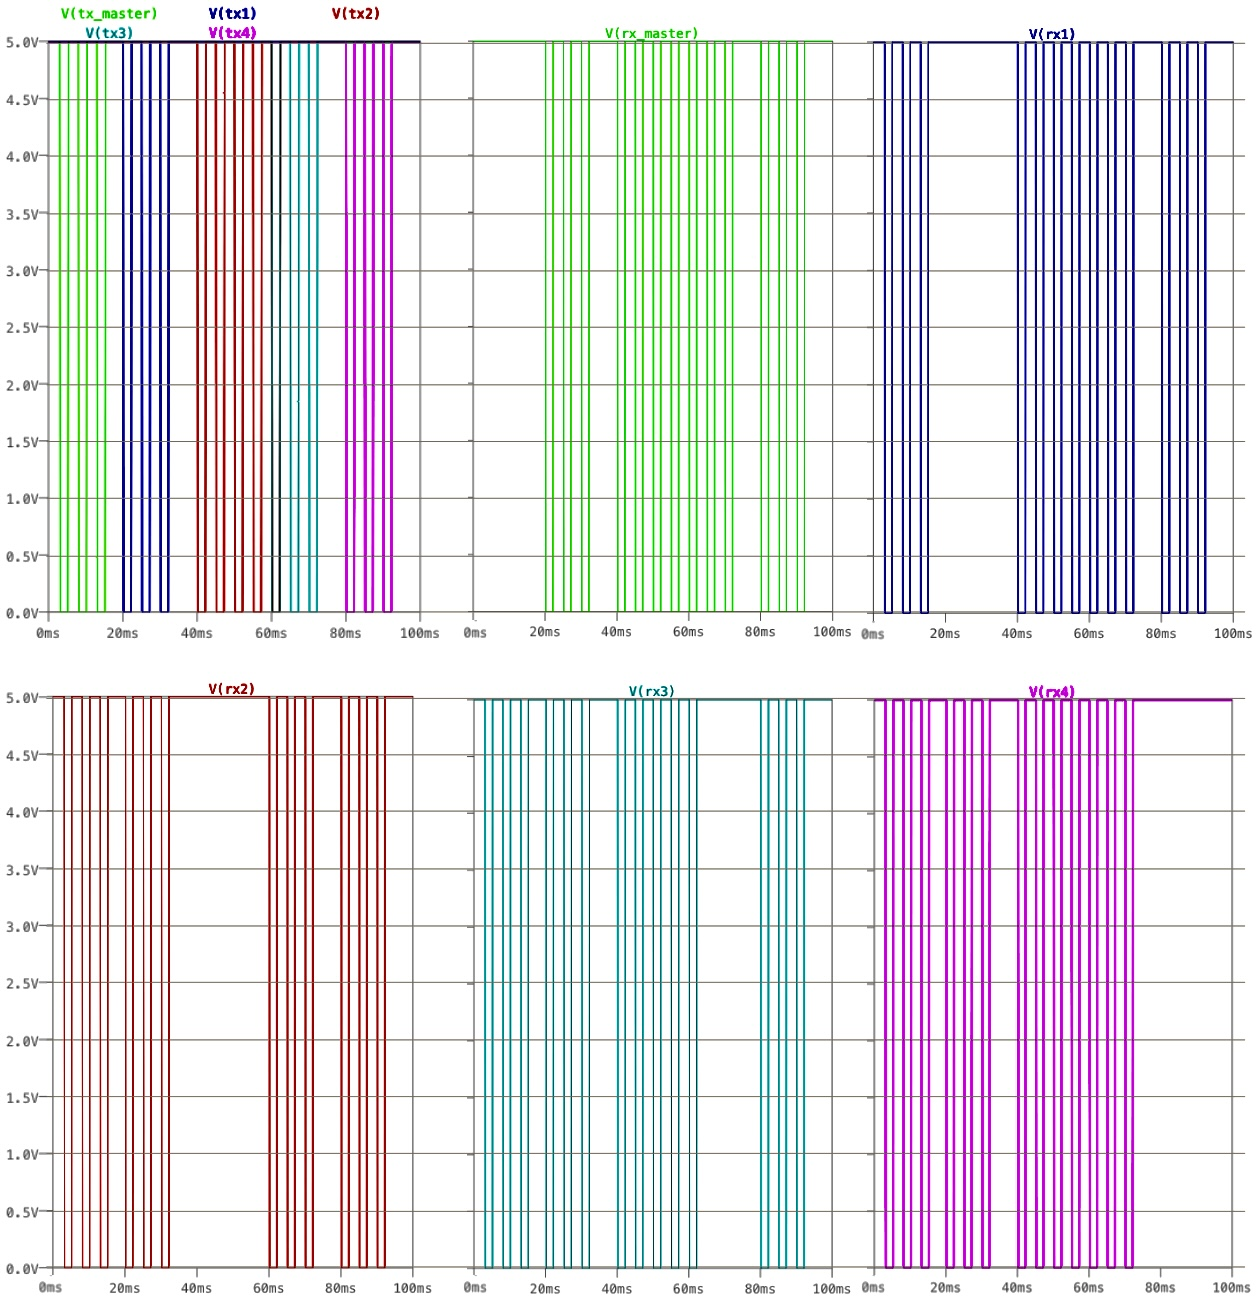
\includegraphics[width=0.72\textwidth]{Skripsie_LaTeXTemplate/Figures/theCOMMStestRES.jpg}
\caption{UART Representative Logic Pulses Measured by ESP32}
\label{fig:comsEXP2}
\end{figure}
%*******************************************%
\subsubsection{UART, Voltage measurement \& Cell Balancing}\label{subsec:CBT}
%*******************************************%
These three monitoring module functions were validated using a test program, as illustrated in the subsequent flow diagram. The module received UART messages while concurrently measuring the cell's live voltage through its microcontroller. This integration enabled the system to activate the balancing dump-load, aligning the cell's discharge to the specified voltage level in comparison with the ADC voltage readings.

\begin{figure}[h!]
\centering
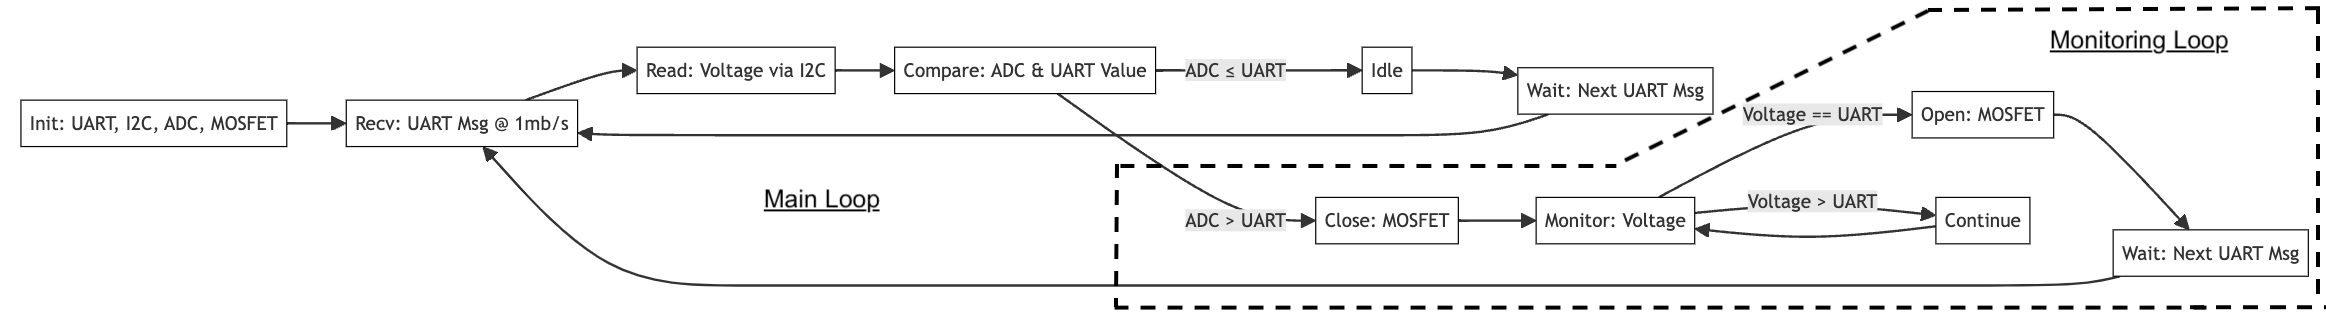
\includegraphics[width=1.0\textwidth]{Skripsie_LaTeXTemplate/Figures/Dumpload_code.png}
\caption{Cell Balancing Test Code Program Flow}
\label{fig:DL_EXP}
\end{figure}
\noindent
The test conducted on the monitoring module affirmed that the system performed in accordance with expectations. The behavior of the system aligned precisely with anticipated outcomes. The ADC provided measurements with a high degree of accuracy, and upon activation, the dump-load circuitry effectively operated at a current of 1A, successfully maintaining the cell voltage at the correct levels throughout the duration of the experiment.\newpage
%*******************************************%
\subsubsection{Controller Current Capability}\label{subsec:Thermal_Test}
%*******************************************%
With assistance from Mr. Petzer, we conducted an experiment using a high-capacity DC power supply and a low-impedance, high-power resistive load. The setup involved connecting the power supply to the main controller board's battery terminals, and the load to the load/charger terminals. The DC isolator successfully separated the power supply side from the load side upon initiation. Engaging the main controller board's relay allowed for a significant 100A current flow. Thermal behavior under these conditions was observed with a Fluke TiS20 thermal camera, as shown in Figure \ref{fig:Thermal}.

\begin{figure}[h!]
\centering
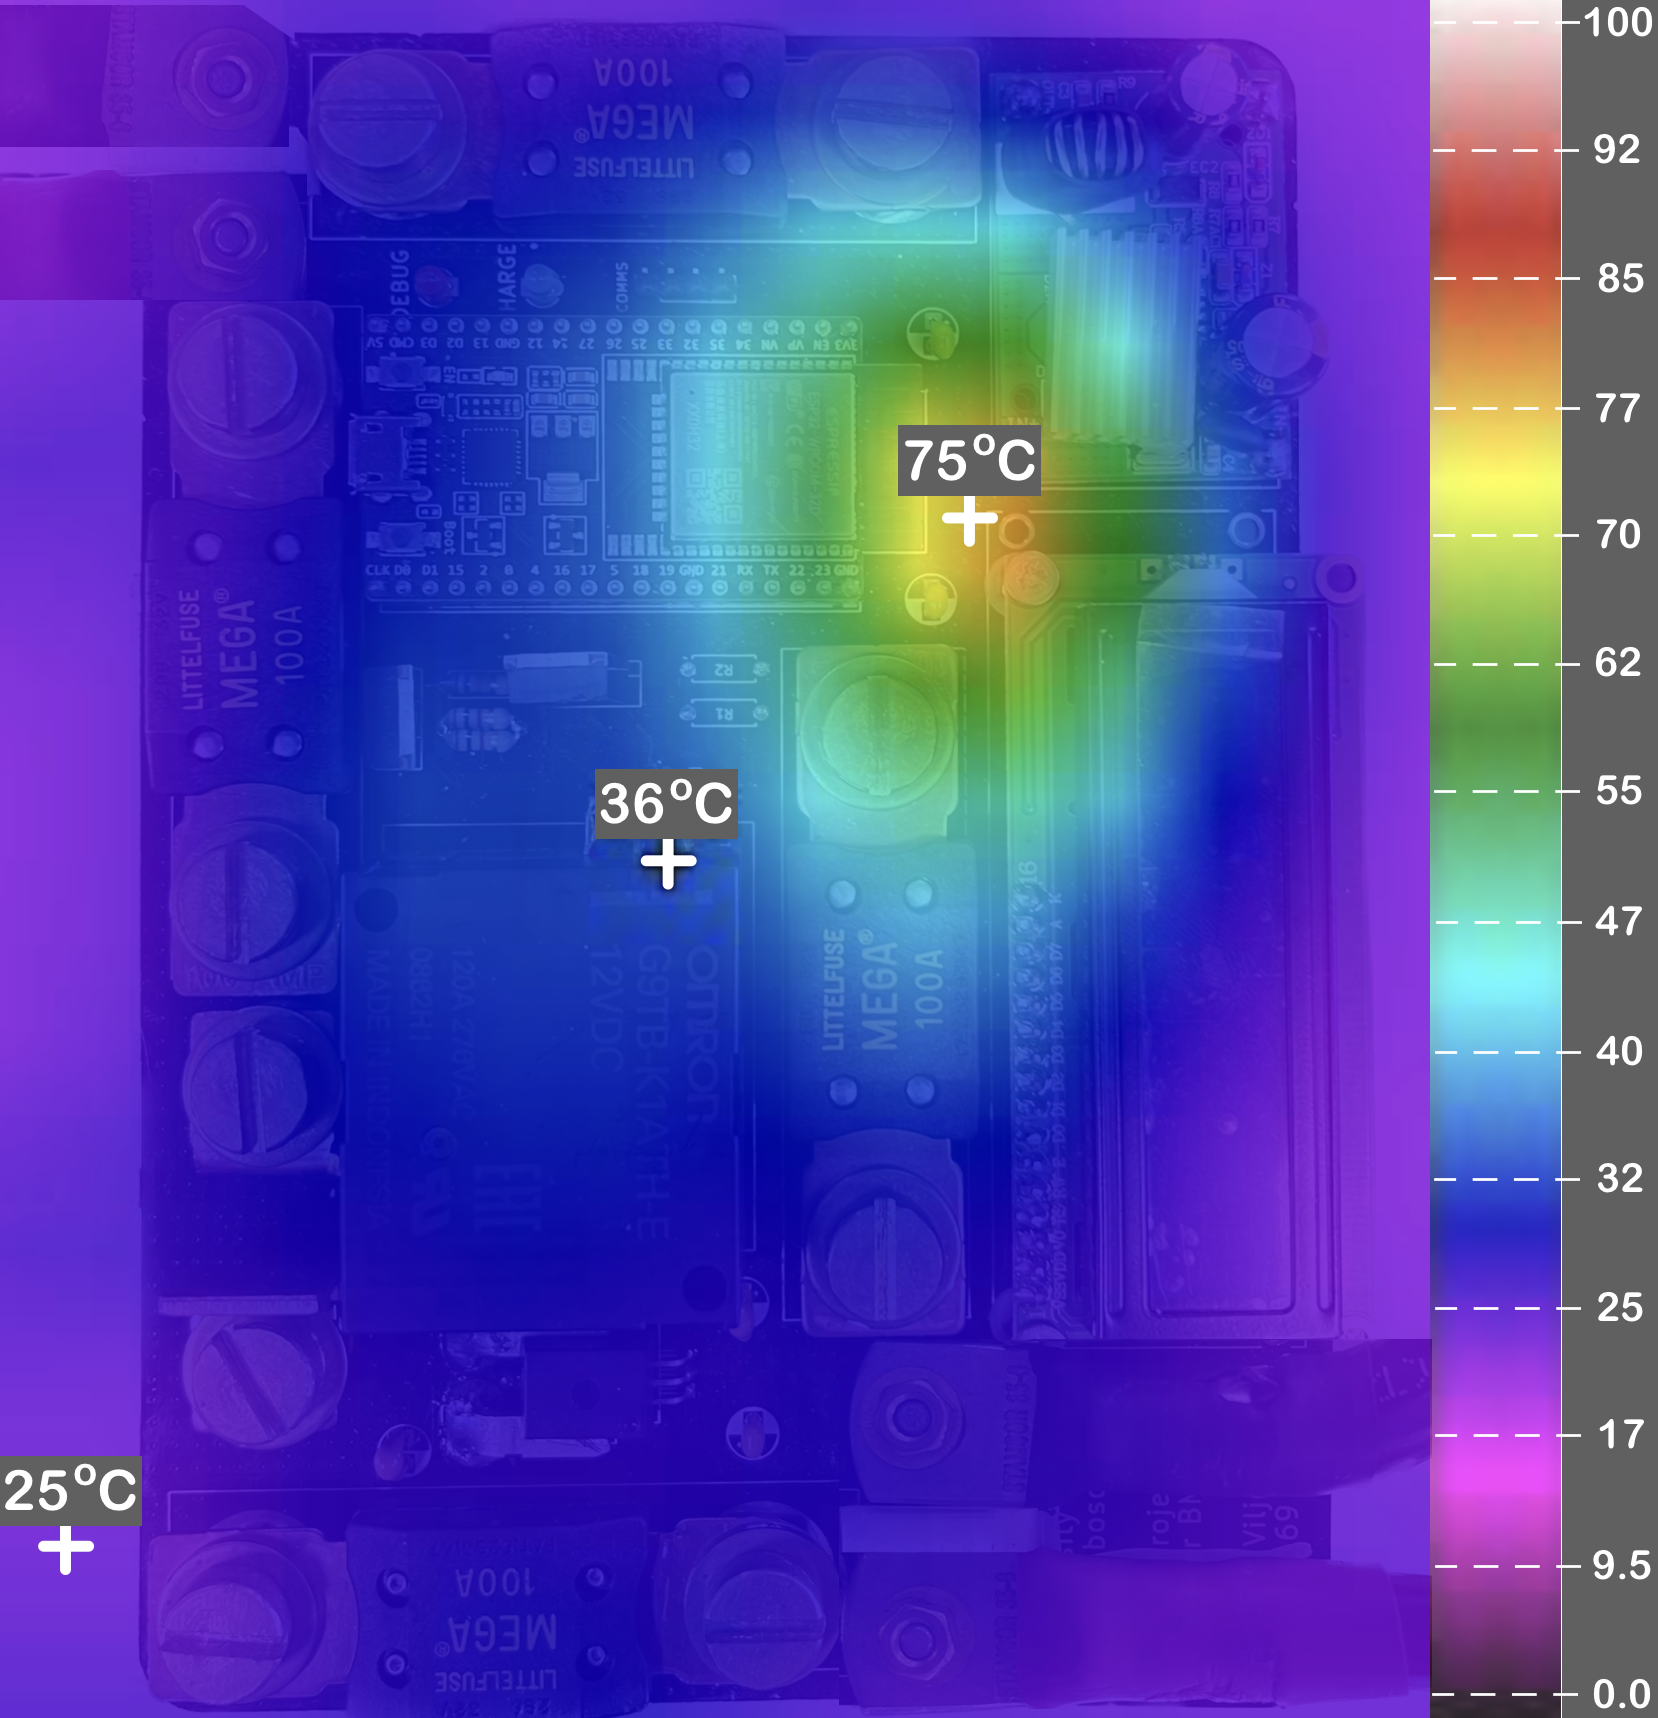
\includegraphics[width=0.4\textwidth]{Figures/thermal_image.png}
\caption{Thermal Imaging with Fluke TiS20}
\label{fig:Thermal}
\end{figure}
\noindent
The thermal image verifies the controller's adequacy in managing the current for both battery and load/charger applications, with a single expected hotspot identified. This hotspot aligns with a known design limitation of the PCB, where a routing constraint for the negative terminal fuses impacted the thermal layout. The current single-sided filled zone with non-connecting vias was a result of this constraint, which was acceptable for the current application. For future enhancements, it is recommended to redesign the PCB to include dual-sided filled zones with via stitching to improve thermal management for high-current operations.
%*******************************************%
\subsubsection{Pulsed Cell Discharge}\label{subsec:pulsemee}
%*******************************************%
The experiment assessed a single 3.2V 100Ah cell's discharge characteristics by connecting it to a $90m\Omega$ load through the main controller, inducing a 35A discharge at 0.33C. The controller executed 17 switch cycles of the DC power relay with a 10-minute pulse width and 25\% duty cycle, to minimize temperature fluctuations and maintain cell stability. Cell voltage and current were meticulously recorded by the monitoring module and logged serially. The collected data was graphically represented to analyze the discharge behavior, as illustrated in Figure \ref{fig:pulsess1}.
\newpage
\begin{figure}[h!]
\centering
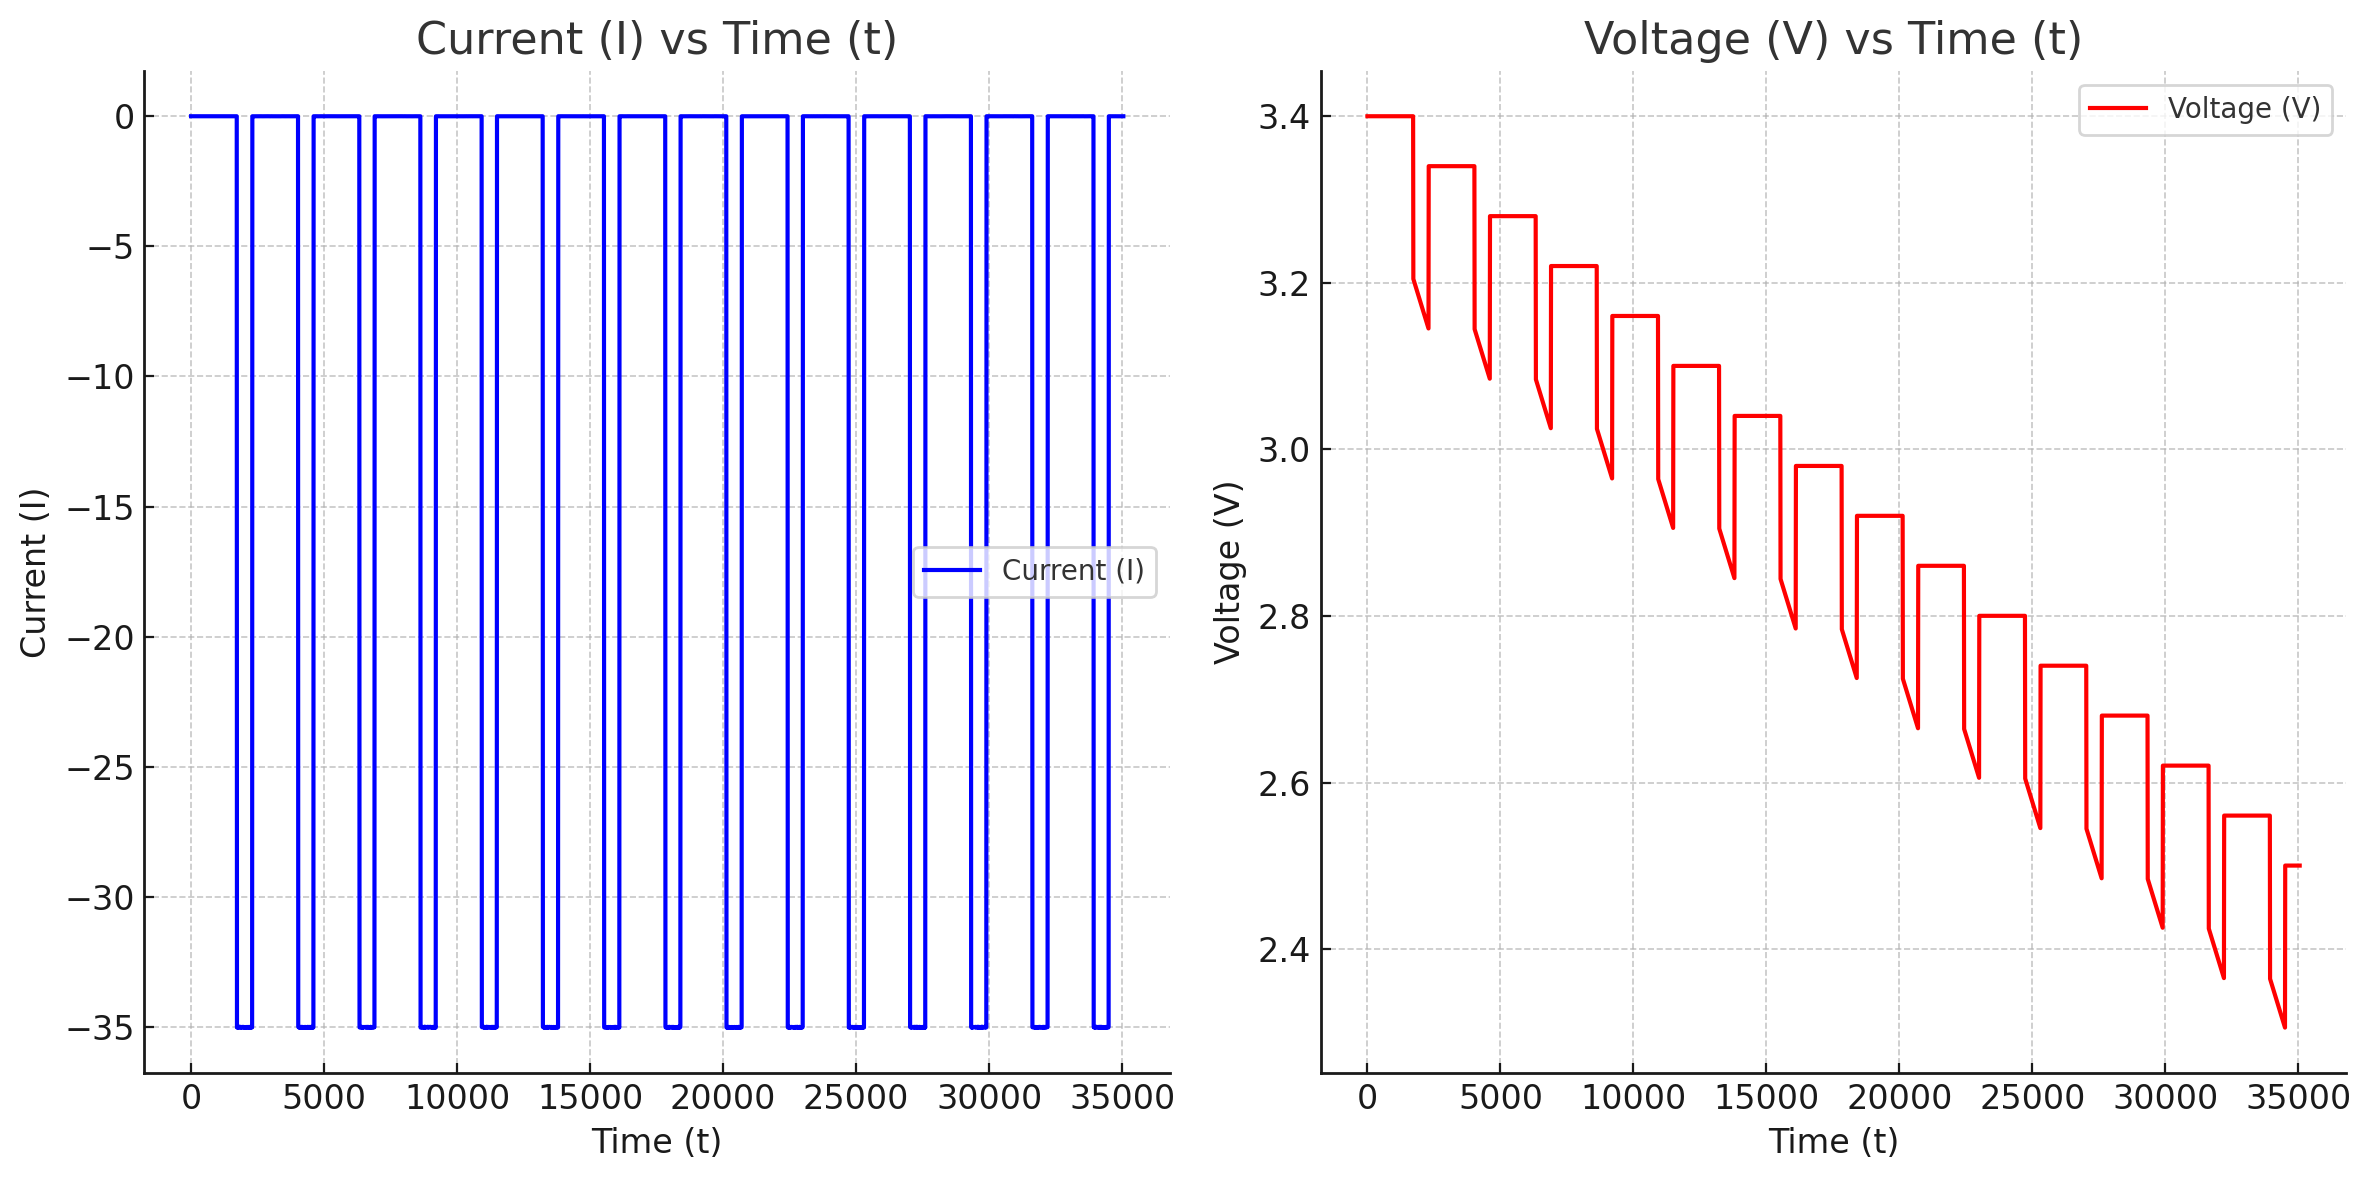
\includegraphics[width=0.6\textwidth]{Skripsie_LaTeXTemplate/Figures/pulseD1.png}
\caption{100Ah 3.2V LFP cell - Pulsed Discharge Current \& Voltage Measured}
\label{fig:pulsess1}
\end{figure}
\noindent
The graphical data from above was imported into MATLAB and analyzed using Javier Gazzarri's battery parameterization model in Simulink \cite{SIMULINKKK}. This facilitated dynamic battery analysis from pulsed discharge data. A modular Battery Management System (BMS) was then developed and simulated in Simulink, utilizing derived parameters to assess system performance. Figure \ref{fig:pulsess2} illustrates the Simulink models and corresponding simulation results. This methodology provided a detailed system evaluation, closely replicating actual battery cell behavior, and confirmed the BMS's operational effectiveness, underscoring Simulink's value in battery system analysis and design.

\begin{figure}[h!]
\centering
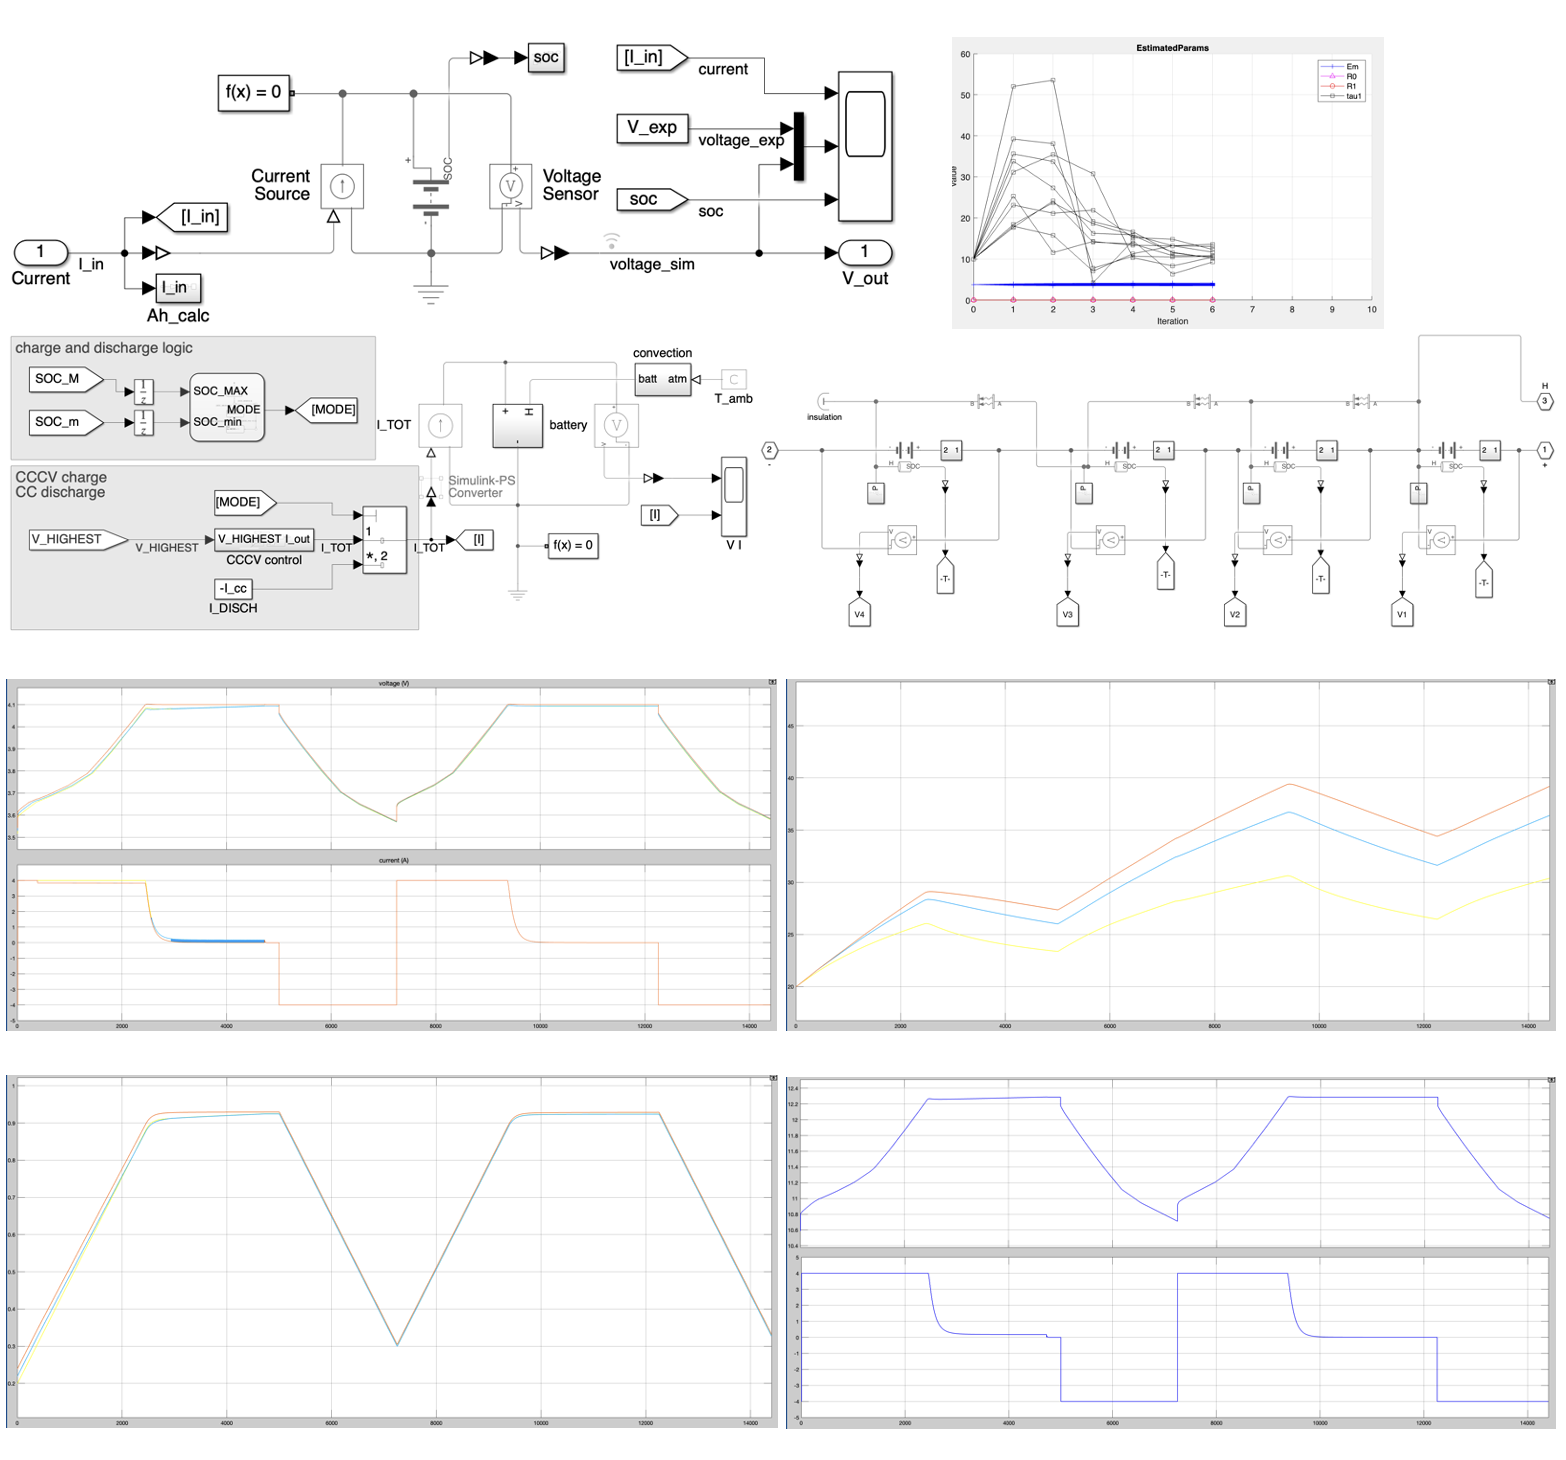
\includegraphics[width=0.8\textwidth]{Skripsie_LaTeXTemplate/Figures/pulseD2.png}
\caption{Simulink Battery Modeling \& Simulated Results \cite{SIMULINKKK}}
\label{fig:pulsess2}
\end{figure}
%*******************************************%


\vfill
\chapter[Conclusion]{Chapter 6: Conclusion}\label{chap:last}%Two pages long, what did you see, what do you imagine?
%*******************************************%
\section{Retrospective Overview}\label{sec:retro_ovv}
%*******************************************%
The crux of a modular BMS is its three core components: the Main Controller's power rating, linking the battery pack with external power lines, the scalable monitoring offered by Cell Modules, and the Module Communication System. Together, they form the heartbeat of the BMS, each playing a pivotal role in the system's overall performance and adaptability. The Main Controller has proven pivotal in integrating energy storage systems with power infrastructures. Cell Modules have brought unparalleled scalability, adapting to diverse energy demands. The Communication System has acted as the crucial link, ensuring cohesive operation and real-time responsiveness.
%*******************************************%
\section{Recommendations and Forward Look}\label{sec:recommend}
%*******************************************%
\textbf{Future Work:} Moving forward, design iterations are essential to reinforce the BMS's robustness and establish a fundamental communication system. The encountered UART communication issues underscore the need for a protocol that scales with the increasing number of microcontrollers. Future enhancements should focus on a scalable protocol, improved user interfaces for diagnostics, and sophisticated algorithms for charge balancing and health assessments, to drive the BMS towards technological and user-centric excellence.
%*******************************************%
\section{Denouement}\label{sec:last_CON}
%*******************************************%
Iterative design methodology is key to achieving a communication system capable of supporting the highest number of cell module microcontrollers. Calculating the power ratings for extensive cell networks and designing a controller for series string disconnect/connect are crucial steps. The design, boxed in unit cell string modules, must be fortified at every layer—starting from the main controllers to the high voltage pinnacle. Each iterative layer adds to the robustness of the foundation, making the cell monitoring module integral in a Modular Battery Management System for LFP Batteries, paving the way for an energy-resilient future.
%*******************************************%

\vfill


% Bibliography
\bibliography{References}

% End matter
\appendix
\chapter{Project Planning Schedule}
\makeatletter\@mkboth{}{Appendix}\makeatother
\label{appen:PP}

\begin{table}[h]
\centering
\begin{tabularx}{\textwidth}{|c|X|c|}
\hline
\textbf{Week} & \textbf{Work Planned to Start} & \textbf{GanttChart Ref.} \\
\hline
1 & Conduct Detailed Research on BMS Topology & Research \\
\hline
2 & Draft Abstract Report & Abstract \\
\hline
3 & Initiate System Design Process & Design \\
\hline
4 & Conduct Extensive Datasheet Consultations & Datasheet \\
\hline
5 & Execute Circuit Designs & Circuit \\
\hline
6 & Source Components \& Initiate Ordering Process & Components \\
\hline
7 & Engage in Printed Circuit Board Design Process & PCB Design \\
\hline
8 & Review \& Revise Circuit and PCB Designs & Review \\
\hline
9 & Place Order for Printed Circuit Board & Order PCB \\
\hline
10 & Solder Components \& Conduct Module Debugging & Debugging \\
\hline
11 & Design Reporting \& System Analysis Testing & Reporting \\
\hline
12 & Evaluation \& Conclusion Reporting & Evaluation \\
\hline
\end{tabularx}
\end{table}
     \begin{figure}[!htb]
     \centering
     	\fbox{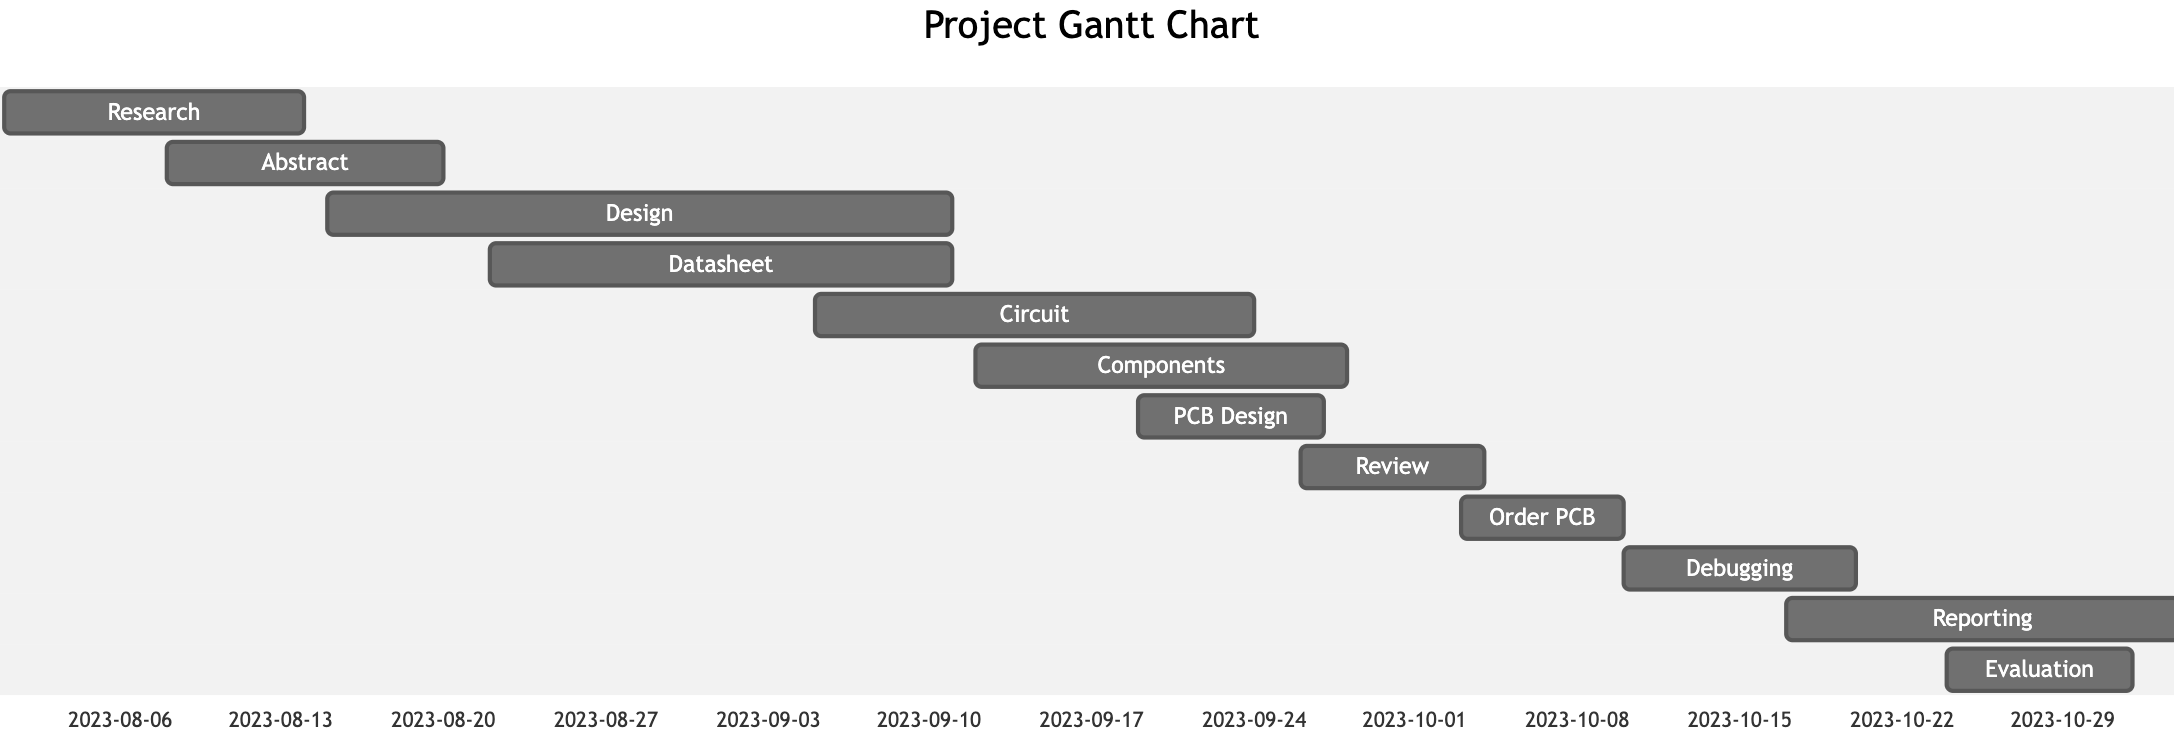
\includegraphics[width=1\linewidth]{./Figures/GanttChart.png}}
	\label{fig:ProjectShed}
	\end{figure}
\chapter{Outcomes Compliance}
\makeatletter\@mkboth{}{Appendix}\makeatother
\label{appen:OC}


\begin{table}[h]
\hspace*{-4cm} %
\caption{ECSA expected learning outcomes (ELO): Descriptions and chapters}
\begin{tabular}{|p{8.5cm}|p{1cm}|p{6.5cm}|}
\hline
\textbf{ECSA Outcome} & \textbf{Ch.} & \textbf{Motivation} \\
\hline
ELO 1. Problem solving: Identify, formulate, analyse and solve complex engineering problems creatively and innovatively. & 1, 3, 4, 5 & Chapters 1 and 3 introduce and conceptualize the problem, Chapter 4 details the design process, and Chapter 5 discusses problem resolution through system evaluation. \\
\hline
ELO 2. Application of scientific and engineering knowledge: Apply knowledge of mathematics, natural sciences, engineering fundamentals and an engineering specialty to solve complex engineering problems. & All & Every chapter contributes to applying scientific and engineering knowledge to develop and refine the BMS. \\
\hline
ELO 3. Engineering Design: Perform creative, procedural and nonprocedural design and synthesis of components, systems, engineering works, products or processes. & 3, 4 & Chapter 3 sets the design requirements, while Chapter 4 provides an in-depth look at the creative and procedural design process. \\
\hline
ELO 4. Investigations, experiments and data analysis: Demonstrate competence to design and conduct investigations and experiments. & 5 & Chapter 5 is dedicated to the evaluation of the system, which includes conducting experiments and analyzing data. \\
\hline
ELO 5. Engineering methods, skills and tools, including Information Technology: Demonstrate competence to use appropriate engineering methods, skills and tools, including those based on information technology. & All & The integration of engineering methods, skills, and IT tools is evident throughout the report. \\
\hline
ELO 6. Professional and technical communication: Demonstrate competence to communicate effectively, both orally and in writing, with engineering audiences and the community at large. & 6 & The conclusion chapter demonstrates the ability to communicate the project's findings and implications effectively. \\
\hline
ELO 8. Individual work: Demonstrate competence to work effectively as an individual. & All & The report, as a whole, is indicative of the author's ability to work independently on a complex engineering project. \\
\hline
ELO 9. Independent Learning Ability: Demonstrate competence to engage in independent learning through well-developed learning skills. & All & The successful completion of the report showcases the author's independent learning abilities throughout the project. \\
\hline
\end{tabular}
\end{table}


\chapter{PCB Cad Assemblies}
\makeatletter\@mkboth{}{Appendix}\makeatother
\label{appen:cad}

     \begin{figure}[!htb]
     \centering
     	\fbox{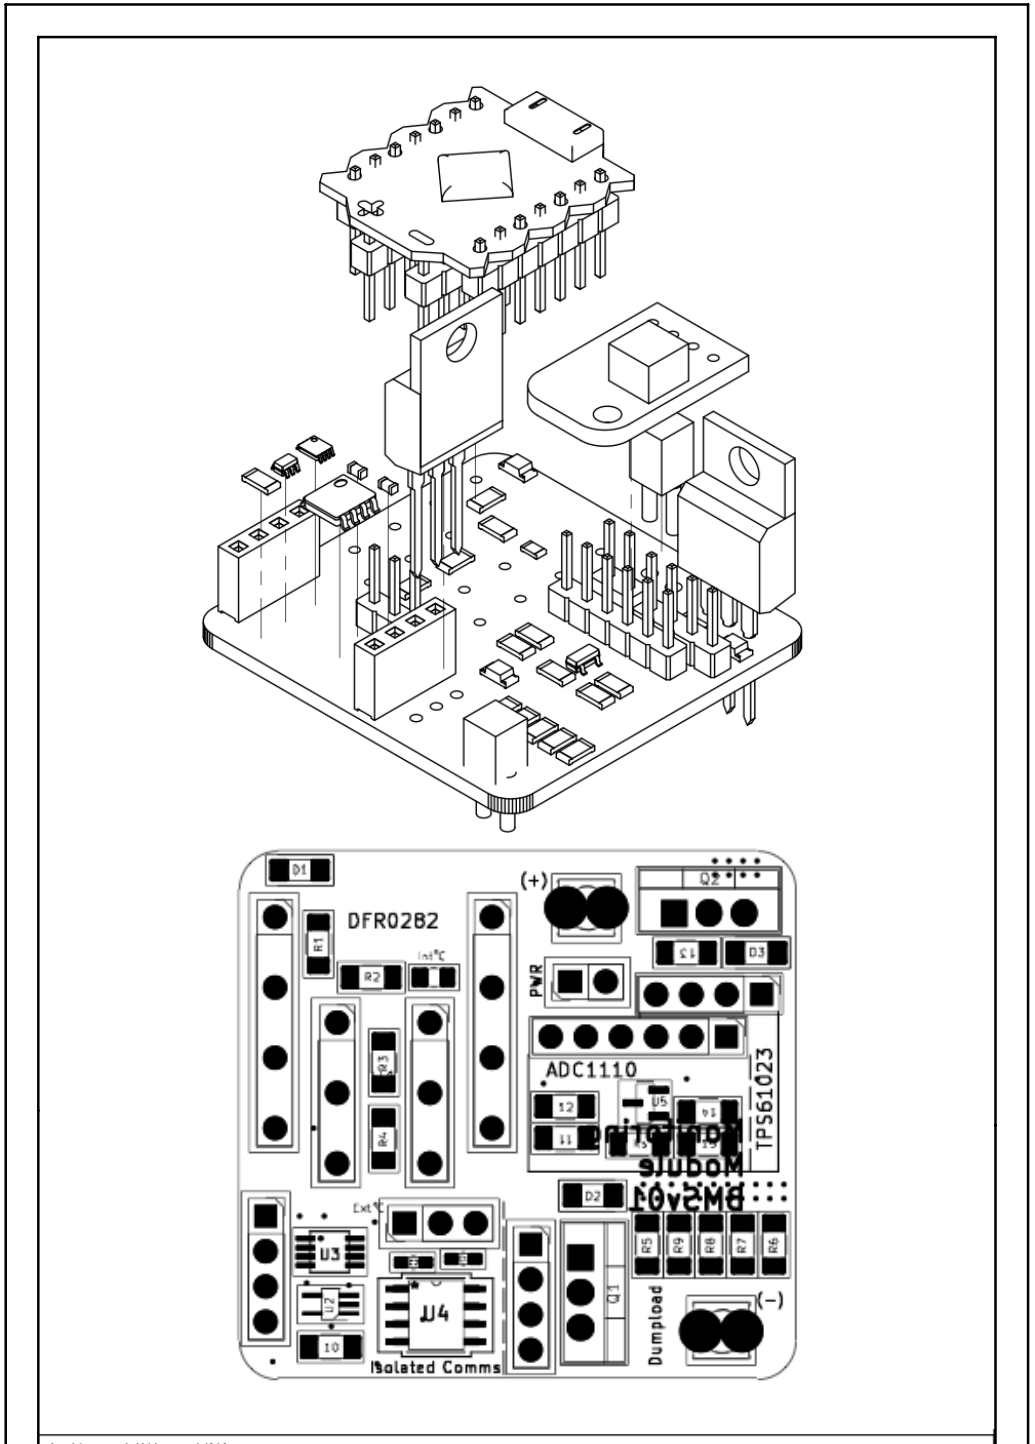
\includegraphics[width=0.9\linewidth]{./Figures/slvCADD.png}}
	\label{fig:cad1}
	\end{figure}

    \begin{figure}[!htb]
     \centering
     	\fbox{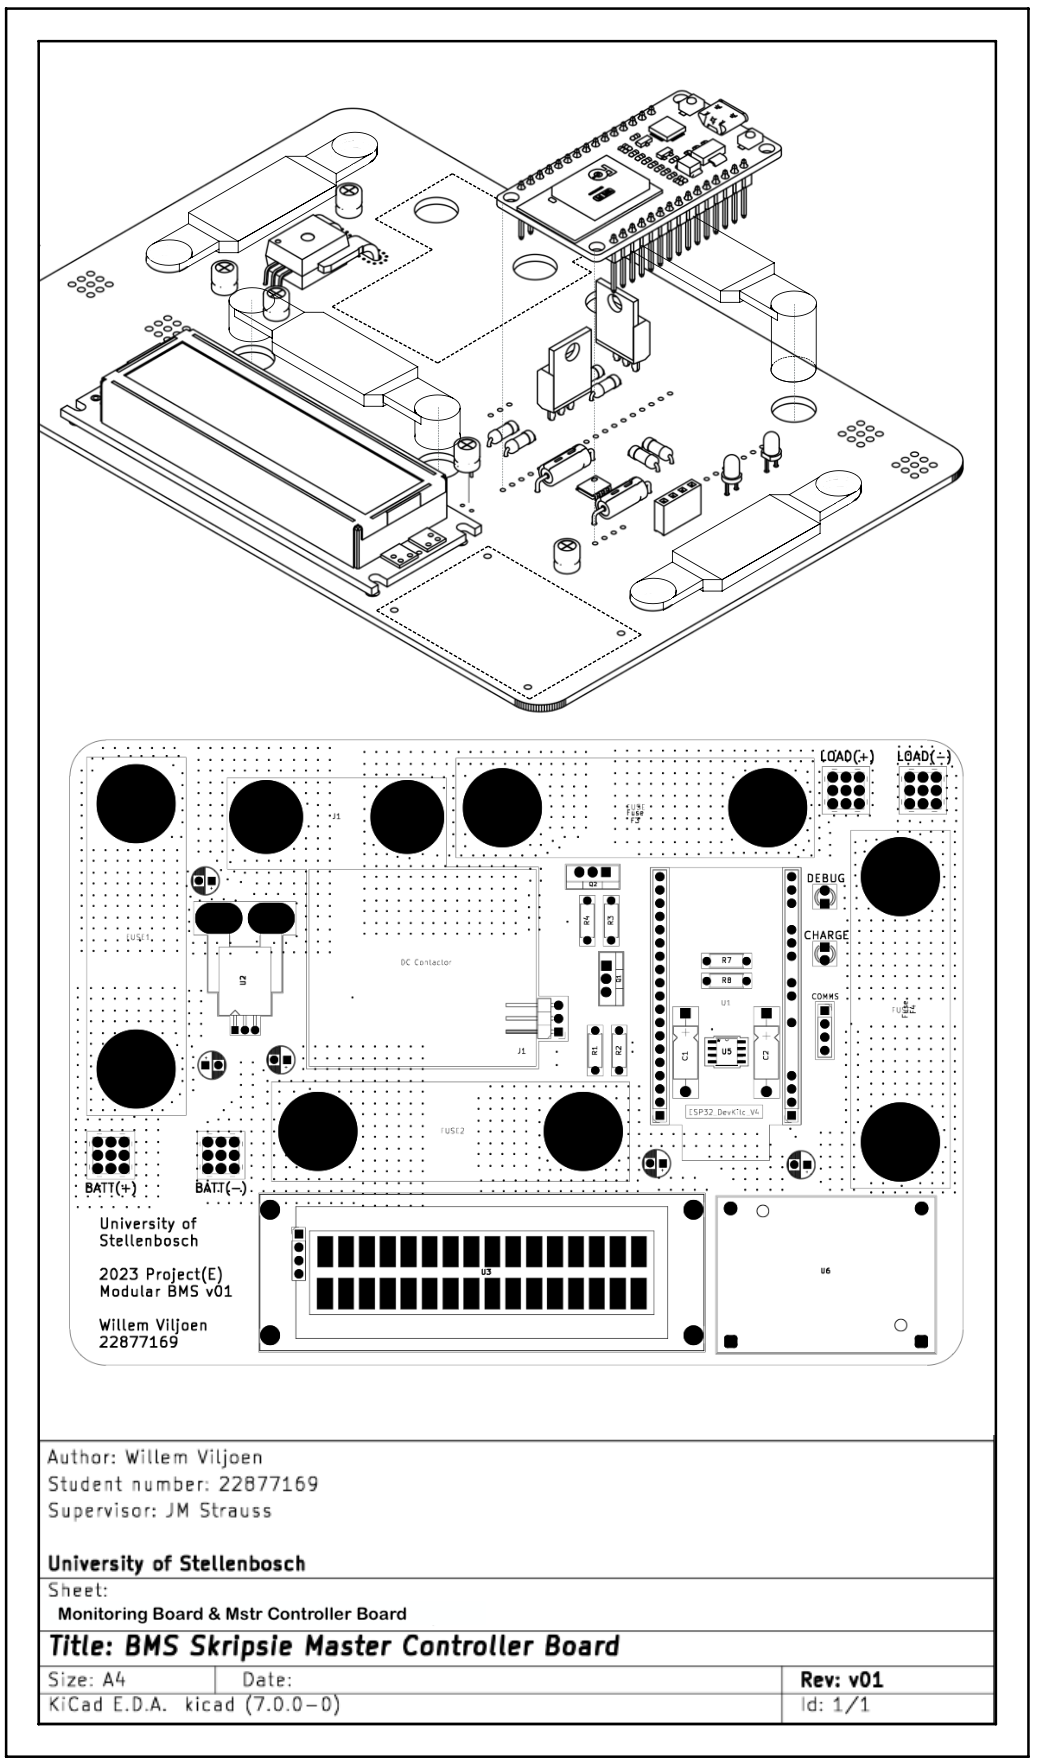
\includegraphics[width=0.9\linewidth]{./Figures/MstrCADD.png}}
	\label{fig:cad2}
	\end{figure}
\chapter{Bill of Materials}
\makeatletter\@mkboth{}{Appendix}\makeatother
\label{appen:BOM}

     \begin{figure}[!htb]
     \centering
     	\fbox{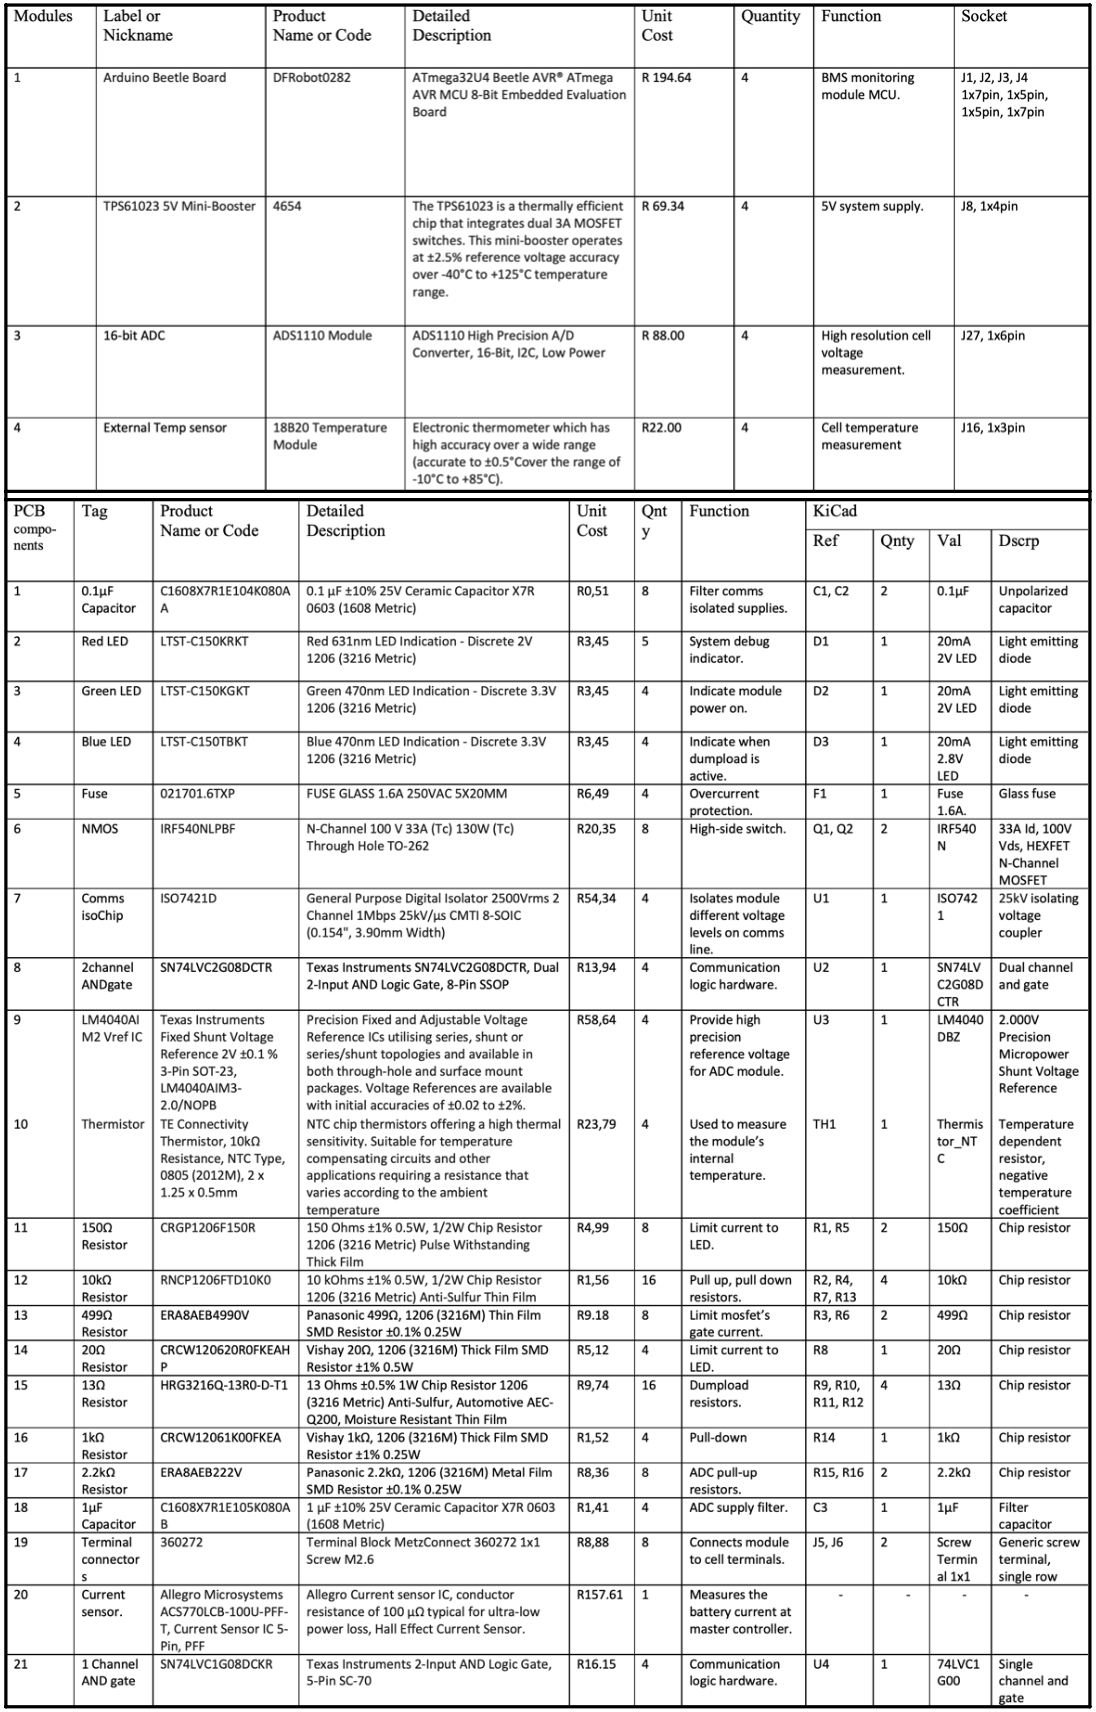
\includegraphics[width=0.89\linewidth]{./Figures/theBOM.png}}
	\label{fig:bom}
	\end{figure}
\chapter*{\textcolor{white}{.}}
\makeatletter\@mkboth{}{Appendix}\makeatother
\label{appen:thanks}
\begin{quote}
    \singlespacing
    {\tiny Special thanks:\newline
    \textcolor{gray}{I would like to take this opportunity to express my deepest gratitude to my Lord and my family for their unwavering support throughout my undergraduate studies. All my success and all my failures belongs to the Lord who gives me strength, thank You for Your grace upon my life. I am particularly grateful to my father for believing in me and funding my undergrad studies, which gave me the opportunity to pursue my dreams. My mother's constant encouragement and support have been invaluable. I would also like to thank my partner for helping me overcome the challenges that I faced during my studies and for having faith in me every step of the way. To everyone who was apart of this 5 year journey of mine, your support has been instrumental in helping me achieve my goals and for that I am grateful.}}
\end{quote}

\end{document}

